\documentclass[a4paper]{book}
\usepackage{a4wide}
\usepackage{makeidx}
\usepackage{graphicx}
\usepackage{multicol}
\usepackage{float}
\usepackage{listings}
\usepackage{color}
\usepackage{textcomp}
\usepackage{alltt}
\usepackage{times}
\usepackage{ifpdf}
\ifpdf
\usepackage[pdftex,
            pagebackref=true,
            colorlinks=true,
            linkcolor=blue,
            unicode
           ]{hyperref}
\else
\usepackage[ps2pdf,
            pagebackref=true,
            colorlinks=true,
            linkcolor=blue,
            unicode
           ]{hyperref}
\usepackage{pspicture}
\fi
\usepackage[utf8]{inputenc}
\usepackage[german]{babel}

\usepackage{doxygen}
\lstset{language=C++,inputencoding=utf8,basicstyle=\footnotesize,breaklines=true,breakatwhitespace=true,tabsize=4,numbers=left }
\makeindex
\setcounter{tocdepth}{3}
\renewcommand{\footrulewidth}{0.4pt}
\begin{document}
\hypersetup{pageanchor=false}
\begin{titlepage}
\vspace*{7cm}
\begin{center}
{\Large CommonDataAnalysis \\[1ex]\large 0.04i }\\
\vspace*{1cm}
{\large Erzeugt von Doxygen 1.6.3}\\
\vspace*{0.5cm}
{\small Thu Jan 20 14:07:32 2011}\\
\end{center}
\end{titlepage}
\clearemptydoublepage
\pagenumbering{roman}
\tableofcontents
\clearemptydoublepage
\pagenumbering{arabic}
\hypersetup{pageanchor=true}
\chapter{libCommonDataAnalysis Documentation}
\label{index}\hypertarget{index}{}\begin{DoxyAuthor}{Autor}
Nils Erik Flick 
\end{DoxyAuthor}

\chapter{Ausstehende Aufgaben}
\label{todo}
\hypertarget{todo}{}
\label{todo__todo000001}
\hypertarget{todo__todo000001}{}
 
\begin{DoxyDescription}
\item[Element \hyperlink{classCDA_1_1EMMbyGradientDescent_ad089403a73bd611cec7b40da92e4adb9}{CDA::EMMbyGradientDescent::preparations\_\-for\_\-evalPDFderivP}()=0 ]refactor! 
\end{DoxyDescription}

\label{todo__todo000002}
\hypertarget{todo__todo000002}{}
 
\begin{DoxyDescription}
\item[Element \hyperlink{classCDA_1_1EMThetas_a1c8058269e4d8a32a2dd58f13ad94369}{CDA::EMThetas::setTheta}(std::pair$<$ II, II $>$ thetas\_\-) ]random numbers when none given 
\end{DoxyDescription}

\label{todo__todo000003}
\hypertarget{todo__todo000003}{}
 
\begin{DoxyDescription}
\item[Element \hyperlink{classCDA_1_1GaussianMixtureModel1D_ada5a646f31d12697bc0fc66934a54dab}{CDA::GaussianMixtureModel1D::setData}(std::pair$<$ II, II $>$ data\_\-) ]we should check II for compliance. 
\end{DoxyDescription}

\label{todo__todo000006}
\hypertarget{todo__todo000006}{}
 
\begin{DoxyDescription}
\item[Element \hyperlink{classCDA_1_1GaussianMixtureModel_a65065aeca55fef7931c83911ca656a3b}{CDA::GaussianMixtureModel::getSigmaDet}(const unsigned k) const  ]urgent avoid re-\/calculations. I'm not saying \char`\"{}memoize\char`\"{} but \char`\"{}be watchful\char`\"{}. 
\end{DoxyDescription}

\label{todo__todo000007}
\hypertarget{todo__todo000007}{}
 
\begin{DoxyDescription}
\item[Datei \hyperlink{ProbabilisticClustering_8c_09_09}{ProbabilisticClustering.c++} ]crippling bugs in multivariate gaussian specialization


\end{DoxyDescription}
\chapter{Klassen-\/Verzeichnis}
\section{Klassenhierarchie}
Die Liste der Ableitungen ist -\/mit Einschränkungen-\/ alphabetisch sortiert:\begin{DoxyCompactList}
\item \contentsline{section}{CDA::compareByVectorElementValue$<$ vector\_\-t, idx\_\-t, LT $>$}{\pageref{structCDA_1_1compareByVectorElementValue}}{}
\item \contentsline{section}{CDA::EM$<$ data\_\-T, theta\_\-T $>$}{\pageref{classCDA_1_1EM}}{}
\begin{DoxyCompactList}
\item \contentsline{section}{CDA::FitMulticlassByEM$<$ data\_\-T, theta\_\-T $>$}{\pageref{classCDA_1_1FitMulticlassByEM}}{}
\end{DoxyCompactList}
\item \contentsline{section}{CDA::EM$<$ EMData$<$ double $>$, EMThetas $>$}{\pageref{classCDA_1_1EM}}{}
\begin{DoxyCompactList}
\item \contentsline{section}{CDA::FitMulticlassByEM$<$ EMData$<$ double $>$, EMThetas $>$}{\pageref{classCDA_1_1FitMulticlassByEM}}{}
\begin{DoxyCompactList}
\item \contentsline{section}{CDA::FitUnivariateMulticlassByEM}{\pageref{classCDA_1_1FitUnivariateMulticlassByEM}}{}
\begin{DoxyCompactList}
\item \contentsline{section}{CDA::GaussianMixtureModel1D}{\pageref{classCDA_1_1GaussianMixtureModel1D}}{}
\end{DoxyCompactList}
\end{DoxyCompactList}
\end{DoxyCompactList}
\item \contentsline{section}{CDA::EM$<$ VectorEMData, GaussianMixtureModelNDParams $>$}{\pageref{classCDA_1_1EM}}{}
\begin{DoxyCompactList}
\item \contentsline{section}{CDA::FitMulticlassByEM$<$ VectorEMData, GaussianMixtureModelNDParams $>$}{\pageref{classCDA_1_1FitMulticlassByEM}}{}
\begin{DoxyCompactList}
\item \contentsline{section}{CDA::FitMultivariateMulticlassByEM$<$ GaussianMixtureModelNDParams $>$}{\pageref{classCDA_1_1FitMultivariateMulticlassByEM}}{}
\begin{DoxyCompactList}
\item \contentsline{section}{CDA::EMGenericMixtureModelCore$<$ GaussianMixtureModelNDParams $>$}{\pageref{classCDA_1_1EMGenericMixtureModelCore}}{}
\begin{DoxyCompactList}
\item \contentsline{section}{CDA::GaussianMixtureModelNDCommon}{\pageref{classCDA_1_1GaussianMixtureModelNDCommon}}{}
\begin{DoxyCompactList}
\item \contentsline{section}{CDA::GaussianMixtureModel}{\pageref{classCDA_1_1GaussianMixtureModel}}{}
\end{DoxyCompactList}
\end{DoxyCompactList}
\end{DoxyCompactList}
\end{DoxyCompactList}
\end{DoxyCompactList}
\item \contentsline{section}{CDA::EM$<$ VectorEMData, theta\_\-T $>$}{\pageref{classCDA_1_1EM}}{}
\begin{DoxyCompactList}
\item \contentsline{section}{CDA::FitMulticlassByEM$<$ VectorEMData, theta\_\-T $>$}{\pageref{classCDA_1_1FitMulticlassByEM}}{}
\begin{DoxyCompactList}
\item \contentsline{section}{CDA::FitMultivariateMulticlassByEM$<$ theta\_\-T $>$}{\pageref{classCDA_1_1FitMultivariateMulticlassByEM}}{}
\begin{DoxyCompactList}
\item \contentsline{section}{CDA::EMGenericMixtureModelCore$<$ theta\_\-T $>$}{\pageref{classCDA_1_1EMGenericMixtureModelCore}}{}
\end{DoxyCompactList}
\end{DoxyCompactList}
\end{DoxyCompactList}
\item \contentsline{section}{CDA::EMData$<$ T $>$}{\pageref{classCDA_1_1EMData}}{}
\item \contentsline{section}{CDA::EMData$<$ double $>$}{\pageref{classCDA_1_1EMData}}{}
\item \contentsline{section}{CDA::EMData$<$ fvector\_\-t $>$}{\pageref{classCDA_1_1EMData}}{}
\begin{DoxyCompactList}
\item \contentsline{section}{CDA::VectorEMData}{\pageref{classCDA_1_1VectorEMData}}{}
\end{DoxyCompactList}
\item \contentsline{section}{CDA::EMThetas}{\pageref{classCDA_1_1EMThetas}}{}
\begin{DoxyCompactList}
\item \contentsline{section}{CDA::GaussianMixtureModelNDParams}{\pageref{classCDA_1_1GaussianMixtureModelNDParams}}{}
\end{DoxyCompactList}
\item \contentsline{section}{CDA::EnhancedDataset}{\pageref{classCDA_1_1EnhancedDataset}}{}
\item \contentsline{section}{CDA::EnhancedDatasetView}{\pageref{classCDA_1_1EnhancedDatasetView}}{}
\item \contentsline{section}{GaussianMixtureModelNDClosedForm}{\pageref{classGaussianMixtureModelNDClosedForm}}{}
\item \contentsline{section}{CDA::VonMises}{\pageref{structCDA_1_1VonMises}}{}
\end{DoxyCompactList}

\chapter{Klassen-\/Verzeichnis}
\section{Auflistung der Klassen}
Hier folgt die Aufzählung aller Klassen, Strukturen, Varianten und Schnittstellen mit einer Kurzbeschreibung:\begin{DoxyCompactList}
\item\contentsline{section}{\hyperlink{classCDA_1_1CircularMixtureModel1D}{CDA::CircularMixtureModel1D} }{\pageref{classCDA_1_1CircularMixtureModel1D}}{}
\item\contentsline{section}{\hyperlink{structCDA_1_1compareByVectorElementValue}{CDA::compareByVectorElementValue$<$ vector\_\-t, idx\_\-t, LT $>$} (Use this as a {\bfseries functor} to compare numbers a and b by the values v\mbox{[}a\mbox{]} and v\mbox{[}b\mbox{]} )}{\pageref{structCDA_1_1compareByVectorElementValue}}{}
\item\contentsline{section}{\hyperlink{classCDA_1_1EM}{CDA::EM$<$ datapoint\_\-t $>$} (A generic \hyperlink{classCDA_1_1EM}{EM} model fitting class. Contains the general outline of \hyperlink{classCDA_1_1EM}{EM} algorithm, details to be filled in by implementations (not that easy in C++ ...) )}{\pageref{classCDA_1_1EM}}{}
\item\contentsline{section}{\hyperlink{classCDA_1_1EMData}{CDA::EMData$<$ T $>$} (Any concrete \hyperlink{classCDA_1_1EM}{EM} subclass \char`\"{}has\_\-a\char`\"{} \hyperlink{classCDA_1_1EMData}{EMData} of the appropriate type (i.e. mono-\/ or multivariate) )}{\pageref{classCDA_1_1EMData}}{}
\item\contentsline{section}{\hyperlink{classCDA_1_1EMGenericMixtureModelCore}{CDA::EMGenericMixtureModelCore} (Ideally, each model knows its data layout, parameter estimators and stuff. There could be a general blueprint for dealing with models which cannot be handled analytically, prompting a gradient search for the MLE step )}{\pageref{classCDA_1_1EMGenericMixtureModelCore}}{}
\item\contentsline{section}{\hyperlink{classCDA_1_1EMMbyGradientDescent}{CDA::EMMbyGradientDescent} (\hyperlink{classCDA_1_1EM}{EM} whose M-\/step is done by gradient descent )}{\pageref{classCDA_1_1EMMbyGradientDescent}}{}
\item\contentsline{section}{\hyperlink{classCDA_1_1EMThetas}{CDA::EMThetas} (Model parameters for \hyperlink{classCDA_1_1EM}{EM} )}{\pageref{classCDA_1_1EMThetas}}{}
\item\contentsline{section}{\hyperlink{classCDA_1_1EnhancedDataset}{CDA::EnhancedDataset} (Aware of basic statistics for normalization etc )}{\pageref{classCDA_1_1EnhancedDataset}}{}
\item\contentsline{section}{\hyperlink{classCDA_1_1EnhancedDatasetView}{CDA::EnhancedDatasetView} }{\pageref{classCDA_1_1EnhancedDatasetView}}{}
\item\contentsline{section}{\hyperlink{classCDA_1_1FitMulticlassByEM}{CDA::FitMulticlassByEM$<$ T $>$} }{\pageref{classCDA_1_1FitMulticlassByEM}}{}
\item\contentsline{section}{\hyperlink{classCDA_1_1FitMultivariateMulticlassByEM}{CDA::FitMultivariateMulticlassByEM} (It's been demoted to a typedef )}{\pageref{classCDA_1_1FitMultivariateMulticlassByEM}}{}
\item\contentsline{section}{\hyperlink{classCDA_1_1GaussianMixtureModel}{CDA::GaussianMixtureModel} (A heteroscedastic N-\/dimensional Gaussian Mixture Model )}{\pageref{classCDA_1_1GaussianMixtureModel}}{}
\item\contentsline{section}{\hyperlink{classCDA_1_1GaussianMixtureModel1D}{CDA::GaussianMixtureModel1D} }{\pageref{classCDA_1_1GaussianMixtureModel1D}}{}
\item\contentsline{section}{\hyperlink{structCDA_1_1VonMises}{CDA::VonMises} }{\pageref{structCDA_1_1VonMises}}{}
\end{DoxyCompactList}

\chapter{Datei-\/Verzeichnis}
\section{Auflistung der Dateien}
Hier folgt die Aufzählung aller dokumentierten Dateien mit einer Kurzbeschreibung:\begin{DoxyCompactList}
\item\contentsline{section}{include/\hyperlink{common__definitions_8h_09_09}{common\_\-definitions.h++} }{\pageref{common__definitions_8h_09_09}}{}
\item\contentsline{section}{include/data/\hyperlink{Data_8h_09_09}{Data.h++} }{\pageref{Data_8h_09_09}}{}
\item\contentsline{section}{include/math/\hyperlink{CircularStatistics_8c_09_09}{CircularStatistics.c++} }{\pageref{CircularStatistics_8c_09_09}}{}
\item\contentsline{section}{include/math/\hyperlink{CircularStatistics_8h_09_09}{CircularStatistics.h++} (Special functions for circular statistics )}{\pageref{CircularStatistics_8h_09_09}}{}
\item\contentsline{section}{include/utils/\hyperlink{comparisons_8h_09_09}{comparisons.h++} }{\pageref{comparisons_8h_09_09}}{}
\item\contentsline{section}{src/expmax/\hyperlink{CircularMixtureModel1D_8h_09_09}{CircularMixtureModel1D.h++} }{\pageref{CircularMixtureModel1D_8h_09_09}}{}
\item\contentsline{section}{src/expmax/\hyperlink{EM_8h_09_09}{EM.h++} }{\pageref{EM_8h_09_09}}{}
\item\contentsline{section}{src/expmax/\hyperlink{EMCustomOptimization_8h_09_09}{EMCustomOptimization.h++} }{\pageref{EMCustomOptimization_8h_09_09}}{}
\item\contentsline{section}{src/expmax/\hyperlink{EMData_8h_09_09}{EMData.h++} }{\pageref{EMData_8h_09_09}}{}
\item\contentsline{section}{src/expmax/\hyperlink{EMGenericMixtureModelCore_8h_09_09}{EMGenericMixtureModelCore.h++} }{\pageref{EMGenericMixtureModelCore_8h_09_09}}{}
\item\contentsline{section}{src/expmax/\hyperlink{EMTheta_8h_09_09}{EMTheta.h++} }{\pageref{EMTheta_8h_09_09}}{}
\item\contentsline{section}{src/expmax/\hyperlink{FitMulticlassByEM_8h_09_09}{FitMulticlassByEM.h++} }{\pageref{FitMulticlassByEM_8h_09_09}}{}
\item\contentsline{section}{src/expmax/\hyperlink{FitMultivariateMulticlassByEM_8h_09_09}{FitMultivariateMulticlassByEM.h++} }{\pageref{FitMultivariateMulticlassByEM_8h_09_09}}{}
\item\contentsline{section}{src/expmax/\hyperlink{GaussianMixtureModel1D_8h_09_09}{GaussianMixtureModel1D.h++} }{\pageref{GaussianMixtureModel1D_8h_09_09}}{}
\item\contentsline{section}{src/expmax/\hyperlink{GaussianMixtureModelND_8h_09_09}{GaussianMixtureModelND.h++} }{\pageref{GaussianMixtureModelND_8h_09_09}}{}
\item\contentsline{section}{src/expmax/\hyperlink{ProbabilisticClustering_8c_09_09}{ProbabilisticClustering.c++} }{\pageref{ProbabilisticClustering_8c_09_09}}{}
\item\contentsline{section}{src/expmax/\hyperlink{ProbabilisticClustering_8h_09_09}{ProbabilisticClustering.h++} }{\pageref{ProbabilisticClustering_8h_09_09}}{}
\item\contentsline{section}{src/math/\hyperlink{numeric__optimization_8c_09_09}{numeric\_\-optimization.c++} }{\pageref{numeric__optimization_8c_09_09}}{}
\item\contentsline{section}{src/math/\hyperlink{numeric__optimization_8h_09_09}{numeric\_\-optimization.h++} }{\pageref{numeric__optimization_8h_09_09}}{}
\end{DoxyCompactList}

\chapter{Klassen-\/Dokumentation}
\hypertarget{structCDA_1_1compareByVectorElementValue}{
\section{CDA::compareByVectorElementValue$<$ vector\_\-t, idx\_\-t, LT $>$ Template-\/Klassenreferenz}
\label{structCDA_1_1compareByVectorElementValue}\index{CDA::compareByVectorElementValue@{CDA::compareByVectorElementValue}}
}


Use this as a {\bfseries functor} to compare numbers a and b by the values v\mbox{[}a\mbox{]} and v\mbox{[}b\mbox{]}.  




{\ttfamily \#include $<$comparisons.h++$>$}

\subsection*{Öffentliche Methoden}
\begin{DoxyCompactItemize}
\item 
\hypertarget{structCDA_1_1compareByVectorElementValue_a9fa53a4855d6f8aeae5e14f63a53bdc2}{
\hyperlink{structCDA_1_1compareByVectorElementValue_a9fa53a4855d6f8aeae5e14f63a53bdc2}{compareByVectorElementValue} (const vector\_\-t \&v)}
\label{structCDA_1_1compareByVectorElementValue_a9fa53a4855d6f8aeae5e14f63a53bdc2}

\begin{DoxyCompactList}\small\item\em Keep a reference of the vector, use it locally. \item\end{DoxyCompactList}\item 
\hypertarget{structCDA_1_1compareByVectorElementValue_a80b11bd2729685221e5ed63b664d36b3}{
bool \hyperlink{structCDA_1_1compareByVectorElementValue_a80b11bd2729685221e5ed63b664d36b3}{operator()} (const idx\_\-t a, const idx\_\-t b)}
\label{structCDA_1_1compareByVectorElementValue_a80b11bd2729685221e5ed63b664d36b3}

\begin{DoxyCompactList}\small\item\em What do you expect? \item\end{DoxyCompactList}\end{DoxyCompactItemize}
\subsection*{Öffentliche Attribute}
\begin{DoxyCompactItemize}
\item 
\hypertarget{structCDA_1_1compareByVectorElementValue_a845fefe0fa9c3ac7df6f968a92711920}{
const vector\_\-t \& \hyperlink{structCDA_1_1compareByVectorElementValue_a845fefe0fa9c3ac7df6f968a92711920}{m\_\-v}}
\label{structCDA_1_1compareByVectorElementValue_a845fefe0fa9c3ac7df6f968a92711920}

\begin{DoxyCompactList}\small\item\em $\ast$reference$\ast$ to the vector \item\end{DoxyCompactList}\end{DoxyCompactItemize}


\subsection{Ausführliche Beschreibung}
\subsubsection*{template$<$class vector\_\-t, class idx\_\-t = size\_\-t, class LT = std::less$<$typename vector\_\-t::value\_\-type$>$$>$ class CDA::compareByVectorElementValue$<$ vector\_\-t, idx\_\-t, LT $>$}

Use this as a {\bfseries functor} to compare numbers a and b by the values v\mbox{[}a\mbox{]} and v\mbox{[}b\mbox{]}. A \char`\"{}strict weak ordering\char`\"{}, as per STL 

Die Dokumentation für diese Klasse wurde erzeugt aufgrund der Datei:\begin{DoxyCompactItemize}
\item 
include/utils/\hyperlink{comparisons_8h_09_09}{comparisons.h++}\end{DoxyCompactItemize}

\hypertarget{classCDA_1_1EM}{
\section{CDA::EM$<$ data\_\-T, theta\_\-T $>$ Template-\/Klassenreferenz}
\label{classCDA_1_1EM}\index{CDA::EM@{CDA::EM}}
}


A generic \hyperlink{classCDA_1_1EM}{EM} model fitting class.  




{\ttfamily \#include $<$EM.h++$>$}



Basisklasse für \hyperlink{classCDA_1_1FitMulticlassByEM}{CDA::FitMulticlassByEM$<$ data\_\-T, theta\_\-T $>$}.



Zusammengehörigkeiten von CDA::EM$<$ data\_\-T, theta\_\-T $>$:\nopagebreak
\begin{figure}[H]
\begin{center}
\leavevmode
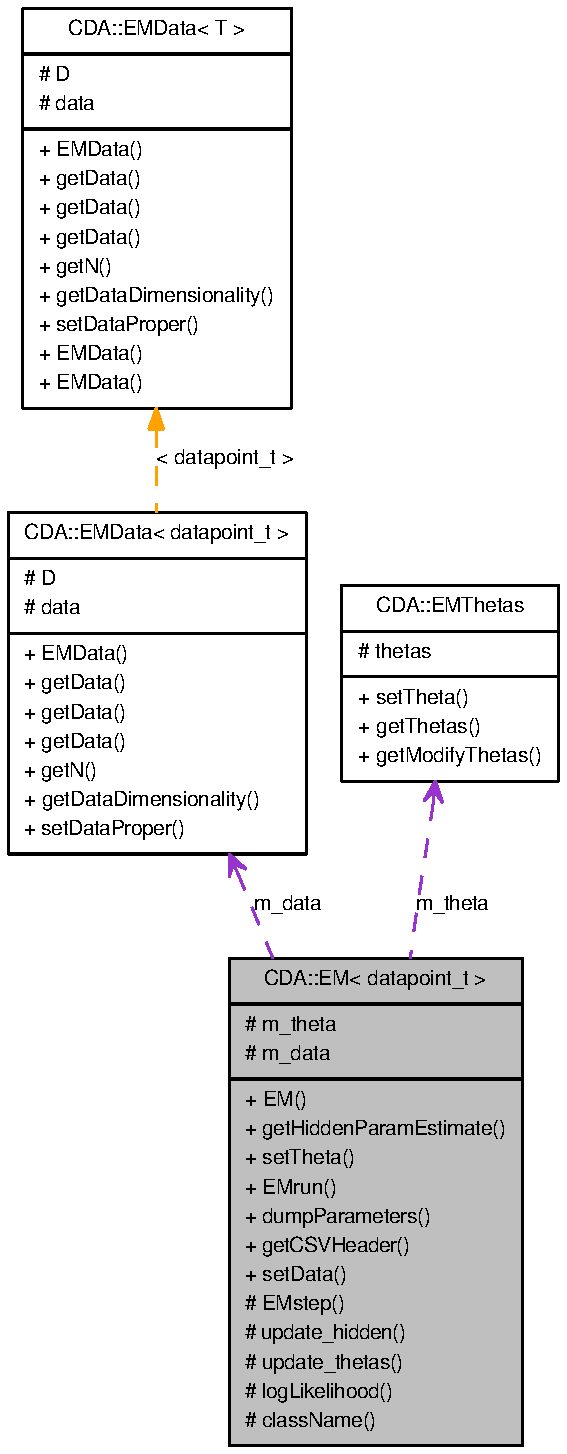
\includegraphics[height=400pt]{classCDA_1_1EM__coll__graph}
\end{center}
\end{figure}
\subsection*{Öffentliche Typen}
\begin{DoxyCompactItemize}
\item 
\hypertarget{classCDA_1_1EM_a3f4735ec5ea6c523ebc4c9f2b51be762}{
typedef data\_\-T \hyperlink{classCDA_1_1EM_a3f4735ec5ea6c523ebc4c9f2b51be762}{data\_\-t}}
\label{classCDA_1_1EM_a3f4735ec5ea6c523ebc4c9f2b51be762}

\begin{DoxyCompactList}\small\item\em Three basic typedefs. \item\end{DoxyCompactList}\item 
\hypertarget{classCDA_1_1EM_a3cdb34eebfa56d948080b28ca349bc6b}{
typedef data\_\-T::value\_\-type {\bfseries datapoint\_\-t}}
\label{classCDA_1_1EM_a3cdb34eebfa56d948080b28ca349bc6b}

\item 
\hypertarget{classCDA_1_1EM_a0f059ae36feb9040200627b78fb416e6}{
typedef theta\_\-T {\bfseries theta\_\-t}}
\label{classCDA_1_1EM_a0f059ae36feb9040200627b78fb416e6}

\end{DoxyCompactItemize}
\subsection*{Öffentliche Methoden}
\begin{DoxyCompactItemize}
\item 
\hyperlink{classCDA_1_1EM_a1b30d405dee72fbf3ef58efffb52add4}{EM} (const \hyperlink{classCDA_1_1EM_a3f4735ec5ea6c523ebc4c9f2b51be762}{data\_\-t} \&data, const theta\_\-t \&theta)
\begin{DoxyCompactList}\small\item\em default constructor \item\end{DoxyCompactList}\item 
\hypertarget{classCDA_1_1EM_a933f9974eec46113eadf9f35ac9b7552}{
\hyperlink{classCDA_1_1EM_a933f9974eec46113eadf9f35ac9b7552}{EM} (const \hyperlink{classCDA_1_1EM}{EM} \&other)}
\label{classCDA_1_1EM_a933f9974eec46113eadf9f35ac9b7552}

\begin{DoxyCompactList}\small\item\em copy constructor Should be implemented throughout \item\end{DoxyCompactList}\item 
\hypertarget{classCDA_1_1EM_aad68b7444dac8fa5e1b0d7413c8ed87c}{
virtual const fvector\_\-t \& \hyperlink{classCDA_1_1EM_aad68b7444dac8fa5e1b0d7413c8ed87c}{getHiddenParamEstimate} (const unsigned n) const =0}
\label{classCDA_1_1EM_aad68b7444dac8fa5e1b0d7413c8ed87c}

\begin{DoxyCompactList}\small\item\em Getter for estimate. \item\end{DoxyCompactList}\item 
void \hyperlink{classCDA_1_1EM_a1c8fa9008da1f168f211f48c578dce5f}{EMrun} (const unsigned MAXITER, const double thresh, const boost::optional$<$ std::ostream $\ast$ $>$ output\_\-csv=boost::none)
\begin{DoxyCompactList}\small\item\em Run Expectation Maximization. \item\end{DoxyCompactList}\item 
virtual const std::string \hyperlink{classCDA_1_1EM_ad2deb0f1d94dc57a6e431caebeb34cbe}{dumpParameters} (const boost::optional$<$ unsigned int $>$ iteration) const =0
\begin{DoxyCompactList}\small\item\em Output CSV. \item\end{DoxyCompactList}\item 
\hypertarget{classCDA_1_1EM_a50155b932fe3a55103550fd69318b45f}{
virtual const std::string \hyperlink{classCDA_1_1EM_a50155b932fe3a55103550fd69318b45f}{getCSVHeader} () const =0}
\label{classCDA_1_1EM_a50155b932fe3a55103550fd69318b45f}

\begin{DoxyCompactList}\small\item\em Möchte es nicht zu kompliziert machen (14/12/2010), daher bekommen die ganzen Klassen erst einmal CSV-\/Ausgabe hardwired. \item\end{DoxyCompactList}\item 
{\footnotesize template$<$class II $>$ }\\void \hyperlink{classCDA_1_1EM_ae71052b178877852d34c3aa17e85f8ef}{setTheta} (std::pair$<$ II, II $>$ thetas)
\begin{DoxyCompactList}\small\item\em Initial guess for model parameters -\/-\/ strictly needed. \item\end{DoxyCompactList}\item 
\hypertarget{classCDA_1_1EM_aa3edb551271b47675c817fa6c302741d}{
virtual const std::string \hyperlink{classCDA_1_1EM_aa3edb551271b47675c817fa6c302741d}{className} () const }
\label{classCDA_1_1EM_aa3edb551271b47675c817fa6c302741d}

\begin{DoxyCompactList}\small\item\em Implementer should overwrite this method, since typeid(this).name() returns crap. \item\end{DoxyCompactList}\item 
unsigned int \hyperlink{classCDA_1_1EM_a12d59d14b42f67805dbf2f721323e318}{getN} () const 
\begin{DoxyCompactList}\small\item\em Return \hyperlink{classCDA_1_1EM_a15809e2026eaea4c68b2e3e11c807fff}{getDataObj()} . \hyperlink{classCDA_1_1EM_a12d59d14b42f67805dbf2f721323e318}{getN()}. \item\end{DoxyCompactList}\end{DoxyCompactItemize}
\subsection*{Geschützte Methoden}
\begin{DoxyCompactItemize}
\item 
virtual \hyperlink{classCDA_1_1EM_a3f4735ec5ea6c523ebc4c9f2b51be762}{data\_\-t} $\ast$ \hyperlink{classCDA_1_1EM_a15809e2026eaea4c68b2e3e11c807fff}{getDataObj} ()
\begin{DoxyCompactList}\small\item\em It's here now. \item\end{DoxyCompactList}\item 
virtual const \hyperlink{classCDA_1_1EM_a3f4735ec5ea6c523ebc4c9f2b51be762}{data\_\-t} $\ast$ \hyperlink{classCDA_1_1EM_ac8ac2e223a295ee8f98e13c50bfec454}{getDataObj} () const 
\begin{DoxyCompactList}\small\item\em Same in const. \item\end{DoxyCompactList}\item 
virtual theta\_\-t $\ast$ \hyperlink{classCDA_1_1EM_aee121bf43a5a5d1a24cfecb2cbd97e18}{getThetaObj} ()
\begin{DoxyCompactList}\small\item\em It's here now. \item\end{DoxyCompactList}\item 
virtual const theta\_\-t $\ast$ \hyperlink{classCDA_1_1EM_aa44545f82da81d3edaee49e34077f58e}{getThetaObj} () const 
\begin{DoxyCompactList}\small\item\em Same in const. \item\end{DoxyCompactList}\item 
double \hyperlink{classCDA_1_1EM_a33684f64b72aff4c65150e12ea23e6aa}{EMstep} ()
\begin{DoxyCompactList}\small\item\em One iteration. \item\end{DoxyCompactList}\item 
\hypertarget{classCDA_1_1EM_a587d80945cad21df1233dc22cb95671d}{
virtual void \hyperlink{classCDA_1_1EM_a587d80945cad21df1233dc22cb95671d}{update\_\-hidden} ()=0}
\label{classCDA_1_1EM_a587d80945cad21df1233dc22cb95671d}

\begin{DoxyCompactList}\small\item\em {\bfseries E-\/step}: update hidden attributes \item\end{DoxyCompactList}\item 
\hypertarget{classCDA_1_1EM_a479e5c57713312a4089e89bb522e2769}{
virtual void \hyperlink{classCDA_1_1EM_a479e5c57713312a4089e89bb522e2769}{update\_\-thetas} ()=0}
\label{classCDA_1_1EM_a479e5c57713312a4089e89bb522e2769}

\begin{DoxyCompactList}\small\item\em {\bfseries M-\/step}: update accessible parameters of model PDF \item\end{DoxyCompactList}\item 
\hypertarget{classCDA_1_1EM_affb4273a70cd7562cc5d517412c4fcdb}{
virtual double \hyperlink{classCDA_1_1EM_affb4273a70cd7562cc5d517412c4fcdb}{logLikelihood} () const =0}
\label{classCDA_1_1EM_affb4273a70cd7562cc5d517412c4fcdb}

\begin{DoxyCompactList}\small\item\em Important. This is being optimized. \item\end{DoxyCompactList}\item 
{\footnotesize template$<$class II $>$ }\\void \hyperlink{classCDA_1_1EM_ad1ee8ed5cef87cfabf708fe8d469b77f}{setData} (std::pair$<$ II, II $>$ data\_\-)
\begin{DoxyCompactList}\small\item\em Initialize known samples, i.e. your data points Also initialize the classif vector. \item\end{DoxyCompactList}\end{DoxyCompactItemize}
\subsection*{Geschützte Attribute}
\begin{DoxyCompactItemize}
\item 
\hypertarget{classCDA_1_1EM_a261037c3e786c1615ea23562a23f3cce}{
\hyperlink{classCDA_1_1EM_a3f4735ec5ea6c523ebc4c9f2b51be762}{data\_\-t} \hyperlink{classCDA_1_1EM_a261037c3e786c1615ea23562a23f3cce}{m\_\-data}}
\label{classCDA_1_1EM_a261037c3e786c1615ea23562a23f3cce}

\begin{DoxyCompactList}\small\item\em We always need this member. Just drop it in via templating, no subclass woes. \item\end{DoxyCompactList}\item 
\hypertarget{classCDA_1_1EM_a64fa0e44a0204dee110cf1095f69ab5c}{
theta\_\-t \hyperlink{classCDA_1_1EM_a64fa0e44a0204dee110cf1095f69ab5c}{m\_\-theta}}
\label{classCDA_1_1EM_a64fa0e44a0204dee110cf1095f69ab5c}

\begin{DoxyCompactList}\small\item\em In C++, \_\-always\_\- works better than inheritance. I should have remembered ... Nevertheless, now you can plug in the appropriate class as a template parameter. \item\end{DoxyCompactList}\end{DoxyCompactItemize}


\subsection{Ausführliche Beschreibung}
\subsubsection*{template$<$class data\_\-T, class theta\_\-T$>$ class CDA::EM$<$ data\_\-T, theta\_\-T $>$}

A generic \hyperlink{classCDA_1_1EM}{EM} model fitting class. \begin{DoxyAuthor}{Autor}
flick
\end{DoxyAuthor}
\hypertarget{GaussianMixtureModel_8h_09_09_Description}{}\subsection{Description}\label{GaussianMixtureModel_8h_09_09_Description}
Contains the general outline of \hyperlink{classCDA_1_1EM}{EM} algorithm, details to be filled in by implementations


\begin{DoxyTemplParams}{Template Parameters}
\item[{\em data\_\-t}]The data-\/point holding class. \item[{\em theta\_\-t}]The model-\/parameter-\/holding class. \end{DoxyTemplParams}


\subsection{Beschreibung der Konstruktoren und Destruktoren}
\hypertarget{classCDA_1_1EM_a1b30d405dee72fbf3ef58efffb52add4}{
\index{CDA::EM@{CDA::EM}!EM@{EM}}
\index{EM@{EM}!CDA::EM@{CDA::EM}}
\subsubsection[{EM}]{\setlength{\rightskip}{0pt plus 5cm}template$<$class data\_\-t , class theta\_\-t $>$ EM::EM (const {\bf data\_\-t} \& {\em data}, \/  const theta\_\-t \& {\em theta})\hspace{0.3cm}{\ttfamily  \mbox{[}inline\mbox{]}}}}
\label{classCDA_1_1EM_a1b30d405dee72fbf3ef58efffb52add4}


default constructor 


\begin{DoxyParams}{Parameter}
\item[\mbox{$\leftarrow$} {\em data\_\-t}](sometimes this needs special initialization) \item[\mbox{$\leftarrow$} {\em theta\_\-t}](sometimes this needs special initialization) \end{DoxyParams}


\subsection{Dokumentation der Elementfunktionen}
\hypertarget{classCDA_1_1EM_ad2deb0f1d94dc57a6e431caebeb34cbe}{
\index{CDA::EM@{CDA::EM}!dumpParameters@{dumpParameters}}
\index{dumpParameters@{dumpParameters}!CDA::EM@{CDA::EM}}
\subsubsection[{dumpParameters}]{\setlength{\rightskip}{0pt plus 5cm}template$<$class data\_\-T, class theta\_\-T$>$ virtual const std::string {\bf CDA::EM}$<$ data\_\-T, theta\_\-T $>$::dumpParameters (const boost::optional$<$ unsigned int $>$ {\em iteration}) const\hspace{0.3cm}{\ttfamily  \mbox{[}pure virtual\mbox{]}}}}
\label{classCDA_1_1EM_ad2deb0f1d94dc57a6e431caebeb34cbe}


Output CSV. 


\begin{DoxyParams}{Parameter}
\item[\mbox{$\leftarrow$} {\em iteration}](optional) output iteration no. in first column \end{DoxyParams}


Implementiert in \hyperlink{classCDA_1_1FitMulticlassByEM_abd04a7135250a427a100c95bf2bf43a9}{CDA::FitMulticlassByEM$<$ data\_\-T, theta\_\-T $>$}, \hyperlink{classCDA_1_1FitMulticlassByEM_abd04a7135250a427a100c95bf2bf43a9}{CDA::FitMulticlassByEM$<$ VectorEMData, GaussianMixtureModelNDParams $>$}, \hyperlink{classCDA_1_1FitMulticlassByEM_abd04a7135250a427a100c95bf2bf43a9}{CDA::FitMulticlassByEM$<$ VectorEMData, theta\_\-T $>$} und \hyperlink{classCDA_1_1FitMulticlassByEM_abd04a7135250a427a100c95bf2bf43a9}{CDA::FitMulticlassByEM$<$ EMData$<$ double $>$, EMThetas $>$}.



Hier ist ein Graph der zeigt, wo diese Funktion aufgerufen wird:\nopagebreak
\begin{figure}[H]
\begin{center}
\leavevmode
\includegraphics[width=154pt]{classCDA_1_1EM_ad2deb0f1d94dc57a6e431caebeb34cbe_icgraph}
\end{center}
\end{figure}


\hypertarget{classCDA_1_1EM_a1c8fa9008da1f168f211f48c578dce5f}{
\index{CDA::EM@{CDA::EM}!EMrun@{EMrun}}
\index{EMrun@{EMrun}!CDA::EM@{CDA::EM}}
\subsubsection[{EMrun}]{\setlength{\rightskip}{0pt plus 5cm}template$<$class data\_\-t , class theta\_\-t $>$ void EM::EMrun (const unsigned {\em MAXITER}, \/  const double {\em thresh}, \/  const boost::optional$<$ std::ostream $\ast$ $>$ {\em output\_\-csv} = {\ttfamily boost::none})\hspace{0.3cm}{\ttfamily  \mbox{[}inline\mbox{]}}}}
\label{classCDA_1_1EM_a1c8fa9008da1f168f211f48c578dce5f}


Run Expectation Maximization. 


\begin{DoxyParams}{Parameter}
\item[\mbox{$\leftarrow$} {\em MAXITER}]up to a certain number of iterations \item[\mbox{$\leftarrow$} {\em thresh}]stop when loglikelihood difference below threshold \item[\mbox{$\leftarrow$} {\em output\_\-csv}]\end{DoxyParams}
\begin{Desc}
\item[\hyperlink{todo__todo000002}{Noch zu erledigen}]replace the ostream with an \hyperlink{classCDA_1_1EnhancedDataset}{EnhancedDataset}. \end{Desc}


Hier ist ein Graph der zeigt, was diese Funktion aufruft:\nopagebreak
\begin{figure}[H]
\begin{center}
\leavevmode
\includegraphics[width=154pt]{classCDA_1_1EM_a1c8fa9008da1f168f211f48c578dce5f_cgraph}
\end{center}
\end{figure}


\hypertarget{classCDA_1_1EM_a33684f64b72aff4c65150e12ea23e6aa}{
\index{CDA::EM@{CDA::EM}!EMstep@{EMstep}}
\index{EMstep@{EMstep}!CDA::EM@{CDA::EM}}
\subsubsection[{EMstep}]{\setlength{\rightskip}{0pt plus 5cm}template$<$class data\_\-T, class theta\_\-T$>$ double {\bf CDA::EM}$<$ data\_\-T, theta\_\-T $>$::EMstep ()\hspace{0.3cm}{\ttfamily  \mbox{[}inline, protected\mbox{]}}}}
\label{classCDA_1_1EM_a33684f64b72aff4c65150e12ea23e6aa}


One iteration. 

\hypertarget{ProbabilisticClustering_8h_09_09_DESCRIPTION}{}\subsection{DESCRIPTION}\label{ProbabilisticClustering_8h_09_09_DESCRIPTION}
This is the basic \hyperlink{classCDA_1_1EM}{EM} (not extended \hyperlink{classCDA_1_1EM}{EM} etc.) algorithm, by virtue of calls to virtual functions you can adapt the procedure to your problem.\hypertarget{classCDA_1_1EM_SIDE-EFFECTS}{}\subsection{SIDE-\/EFFECTS}\label{classCDA_1_1EM_SIDE-EFFECTS}
This will update the model parameters stored in the \hyperlink{classCDA_1_1EMThetas}{EMThetas} class.

\begin{DoxyReturn}{Rückgabe}
The new log-\/likelihood value after performing the iteration. 
\end{DoxyReturn}


Hier ist ein Graph der zeigt, wo diese Funktion aufgerufen wird:\nopagebreak
\begin{figure}[H]
\begin{center}
\leavevmode
\includegraphics[width=134pt]{classCDA_1_1EM_a33684f64b72aff4c65150e12ea23e6aa_icgraph}
\end{center}
\end{figure}


\hypertarget{classCDA_1_1EM_ac8ac2e223a295ee8f98e13c50bfec454}{
\index{CDA::EM@{CDA::EM}!getDataObj@{getDataObj}}
\index{getDataObj@{getDataObj}!CDA::EM@{CDA::EM}}
\subsubsection[{getDataObj}]{\setlength{\rightskip}{0pt plus 5cm}template$<$class data\_\-t , class theta\_\-t $>$ const {\bf data\_\-t} $\ast$ EM::getDataObj () const\hspace{0.3cm}{\ttfamily  \mbox{[}inline, protected, virtual\mbox{]}}}}
\label{classCDA_1_1EM_ac8ac2e223a295ee8f98e13c50bfec454}


Same in const. 

\hypertarget{GaussianMixtureModel1D_8h_09_09_NOTE}{}\subsection{NOTE}\label{GaussianMixtureModel1D_8h_09_09_NOTE}
It's virtual for historic reasons, don't replace it

\begin{DoxyReturn}{Rückgabe}
reference to datapoints-\/holding object 
\end{DoxyReturn}
\hypertarget{classCDA_1_1EM_a15809e2026eaea4c68b2e3e11c807fff}{
\index{CDA::EM@{CDA::EM}!getDataObj@{getDataObj}}
\index{getDataObj@{getDataObj}!CDA::EM@{CDA::EM}}
\subsubsection[{getDataObj}]{\setlength{\rightskip}{0pt plus 5cm}template$<$class data\_\-t , class theta\_\-t $>$ {\bf data\_\-t} $\ast$ EM::getDataObj ()\hspace{0.3cm}{\ttfamily  \mbox{[}inline, protected, virtual\mbox{]}}}}
\label{classCDA_1_1EM_a15809e2026eaea4c68b2e3e11c807fff}


It's here now. 

\hypertarget{GaussianMixtureModel1D_8h_09_09_NOTE}{}\subsection{NOTE}\label{GaussianMixtureModel1D_8h_09_09_NOTE}
It's virtual for historic reasons, don't replace it

\begin{DoxyReturn}{Rückgabe}
m\_\-data 
\end{DoxyReturn}


Hier ist ein Graph der zeigt, wo diese Funktion aufgerufen wird:\nopagebreak
\begin{figure}[H]
\begin{center}
\leavevmode
\includegraphics[width=420pt]{classCDA_1_1EM_a15809e2026eaea4c68b2e3e11c807fff_icgraph}
\end{center}
\end{figure}


\hypertarget{classCDA_1_1EM_a12d59d14b42f67805dbf2f721323e318}{
\index{CDA::EM@{CDA::EM}!getN@{getN}}
\index{getN@{getN}!CDA::EM@{CDA::EM}}
\subsubsection[{getN}]{\setlength{\rightskip}{0pt plus 5cm}template$<$class data\_\-t , class theta\_\-t $>$ unsigned int EM::getN () const\hspace{0.3cm}{\ttfamily  \mbox{[}inline\mbox{]}}}}
\label{classCDA_1_1EM_a12d59d14b42f67805dbf2f721323e318}


Return \hyperlink{classCDA_1_1EM_a15809e2026eaea4c68b2e3e11c807fff}{getDataObj()} . \hyperlink{classCDA_1_1EM_a12d59d14b42f67805dbf2f721323e318}{getN()}. 

\begin{DoxyReturn}{Rückgabe}
Number of data points 
\end{DoxyReturn}


Hier ist ein Graph der zeigt, was diese Funktion aufruft:\nopagebreak
\begin{figure}[H]
\begin{center}
\leavevmode
\includegraphics[width=138pt]{classCDA_1_1EM_a12d59d14b42f67805dbf2f721323e318_cgraph}
\end{center}
\end{figure}




Hier ist ein Graph der zeigt, wo diese Funktion aufgerufen wird:\nopagebreak
\begin{figure}[H]
\begin{center}
\leavevmode
\includegraphics[width=355pt]{classCDA_1_1EM_a12d59d14b42f67805dbf2f721323e318_icgraph}
\end{center}
\end{figure}


\hypertarget{classCDA_1_1EM_aa44545f82da81d3edaee49e34077f58e}{
\index{CDA::EM@{CDA::EM}!getThetaObj@{getThetaObj}}
\index{getThetaObj@{getThetaObj}!CDA::EM@{CDA::EM}}
\subsubsection[{getThetaObj}]{\setlength{\rightskip}{0pt plus 5cm}template$<$class data\_\-t , class theta\_\-t $>$ const theta\_\-t $\ast$ EM::getThetaObj () const\hspace{0.3cm}{\ttfamily  \mbox{[}inline, protected, virtual\mbox{]}}}}
\label{classCDA_1_1EM_aa44545f82da81d3edaee49e34077f58e}


Same in const. 

\hypertarget{GaussianMixtureModel1D_8h_09_09_NOTE}{}\subsection{NOTE}\label{GaussianMixtureModel1D_8h_09_09_NOTE}
It's virtual for historic reasons, don't replace it

\begin{DoxyReturn}{Rückgabe}
reference to parameter-\/holding object 
\end{DoxyReturn}
\hypertarget{classCDA_1_1EM_aee121bf43a5a5d1a24cfecb2cbd97e18}{
\index{CDA::EM@{CDA::EM}!getThetaObj@{getThetaObj}}
\index{getThetaObj@{getThetaObj}!CDA::EM@{CDA::EM}}
\subsubsection[{getThetaObj}]{\setlength{\rightskip}{0pt plus 5cm}template$<$class data\_\-t , class theta\_\-t $>$ theta\_\-t $\ast$ EM::getThetaObj ()\hspace{0.3cm}{\ttfamily  \mbox{[}inline, protected, virtual\mbox{]}}}}
\label{classCDA_1_1EM_aee121bf43a5a5d1a24cfecb2cbd97e18}


It's here now. 

\hypertarget{GaussianMixtureModel1D_8h_09_09_NOTE}{}\subsection{NOTE}\label{GaussianMixtureModel1D_8h_09_09_NOTE}
It's virtual for historic reasons, don't replace it

\begin{DoxyReturn}{Rückgabe}
m\_\-theta 
\end{DoxyReturn}


Hier ist ein Graph der zeigt, wo diese Funktion aufgerufen wird:\nopagebreak
\begin{figure}[H]
\begin{center}
\leavevmode
\includegraphics[width=320pt]{classCDA_1_1EM_aee121bf43a5a5d1a24cfecb2cbd97e18_icgraph}
\end{center}
\end{figure}


\hypertarget{classCDA_1_1EM_ad1ee8ed5cef87cfabf708fe8d469b77f}{
\index{CDA::EM@{CDA::EM}!setData@{setData}}
\index{setData@{setData}!CDA::EM@{CDA::EM}}
\subsubsection[{setData}]{\setlength{\rightskip}{0pt plus 5cm}template$<$class data\_\-T, class theta\_\-T$>$ template$<$class II $>$ void {\bf CDA::EM}$<$ data\_\-T, theta\_\-T $>$::setData (std::pair$<$ II, II $>$ {\em data\_\-})\hspace{0.3cm}{\ttfamily  \mbox{[}inline, protected\mbox{]}}}}
\label{classCDA_1_1EM_ad1ee8ed5cef87cfabf708fe8d469b77f}


Initialize known samples, i.e. your data points Also initialize the classif vector. 



II must iterate over datapoint\_\-t elements: 



Erneute Implementation in \hyperlink{classCDA_1_1FitMulticlassByEM_a7247bfcad3c828f9cf372b6c414e93f0}{CDA::FitMulticlassByEM$<$ data\_\-T, theta\_\-T $>$}, \hyperlink{classCDA_1_1GaussianMixtureModel1D_ada5a646f31d12697bc0fc66934a54dab}{CDA::GaussianMixtureModel1D}, \hyperlink{classCDA_1_1FitMulticlassByEM_a7247bfcad3c828f9cf372b6c414e93f0}{CDA::FitMulticlassByEM$<$ VectorEMData, GaussianMixtureModelNDParams $>$}, \hyperlink{classCDA_1_1FitMulticlassByEM_a7247bfcad3c828f9cf372b6c414e93f0}{CDA::FitMulticlassByEM$<$ VectorEMData, theta\_\-T $>$} und \hyperlink{classCDA_1_1FitMulticlassByEM_a7247bfcad3c828f9cf372b6c414e93f0}{CDA::FitMulticlassByEM$<$ EMData$<$ double $>$, EMThetas $>$}.

\hypertarget{classCDA_1_1EM_ae71052b178877852d34c3aa17e85f8ef}{
\index{CDA::EM@{CDA::EM}!setTheta@{setTheta}}
\index{setTheta@{setTheta}!CDA::EM@{CDA::EM}}
\subsubsection[{setTheta}]{\setlength{\rightskip}{0pt plus 5cm}template$<$class data\_\-T, class theta\_\-T$>$ template$<$class II $>$ void {\bf CDA::EM}$<$ data\_\-T, theta\_\-T $>$::setTheta (std::pair$<$ II, II $>$ {\em thetas})\hspace{0.3cm}{\ttfamily  \mbox{[}inline\mbox{]}}}}
\label{classCDA_1_1EM_ae71052b178877852d34c3aa17e85f8ef}


Initial guess for model parameters -\/-\/ strictly needed. 

\hypertarget{classCDA_1_1GaussianMixtureModelNDParams_NOTA}{}\subsection{BENE}\label{classCDA_1_1GaussianMixtureModelNDParams_NOTA}
Input data format differs for each individual distribution, be careful and read the documentation. Should be in protected


\begin{DoxyParams}{Parameter}
\item[\mbox{$\leftarrow$} {\em thetas}]\end{DoxyParams}


Die Dokumentation für diese Klasse wurde erzeugt aufgrund der Dateien:\begin{DoxyCompactItemize}
\item 
include/expmax/\hyperlink{EM_8h_09_09}{EM.h++}\item 
src/expmax/\hyperlink{EM_8c_09_09}{EM.c++}\end{DoxyCompactItemize}

\hypertarget{classCDA_1_1EMData}{
\section{CDA::EMData$<$ T $>$ Template-\/Klassenreferenz}
\label{classCDA_1_1EMData}\index{CDA::EMData@{CDA::EMData}}
}


Any concrete \hyperlink{classCDA_1_1EM}{EM} subclass \char`\"{}has\_\-a\char`\"{} \hyperlink{classCDA_1_1EMData}{EMData} of the appropriate type (i.e. mono-\/ or multivariate).  




{\ttfamily \#include $<$EMData.h++$>$}

\subsection*{Öffentliche Typen}
\begin{DoxyCompactItemize}
\item 
typedef T \hyperlink{classCDA_1_1EMData_a320dfbd3ad13091a99602a140688a05d}{datapoint\_\-t}
\end{DoxyCompactItemize}
\subsection*{Öffentliche Methoden}
\begin{DoxyCompactItemize}
\item 
\hyperlink{classCDA_1_1EMData_ae81ba273dcb87842699fcc1f6bd7b62a}{EMData} (const unsigned D\_\-=1)
\begin{DoxyCompactList}\small\item\em Constructor. \item\end{DoxyCompactList}\item 
\hypertarget{classCDA_1_1EMData_a0f776db698fe3871ed20a6e9af2a37ad}{
const std::vector$<$ \hyperlink{classCDA_1_1EMData_a320dfbd3ad13091a99602a140688a05d}{datapoint\_\-t} $>$ \& \hyperlink{classCDA_1_1EMData_a0f776db698fe3871ed20a6e9af2a37ad}{getData} () const }
\label{classCDA_1_1EMData_a0f776db698fe3871ed20a6e9af2a37ad}

\begin{DoxyCompactList}\small\item\em Const getter. \item\end{DoxyCompactList}\item 
const \hyperlink{classCDA_1_1EMData_a320dfbd3ad13091a99602a140688a05d}{datapoint\_\-t} \& \hyperlink{classCDA_1_1EMData_ab1acf83827d4595d2cb68c90bf7fa175}{getData} (const unsigned n) const 
\begin{DoxyCompactList}\small\item\em Get one data point. \item\end{DoxyCompactList}\item 
\hypertarget{classCDA_1_1EMData_aaab989fb0f59c828ce0c82ffaa36aace}{
std::vector$<$ \hyperlink{classCDA_1_1EMData_a320dfbd3ad13091a99602a140688a05d}{datapoint\_\-t} $>$ \& \hyperlink{classCDA_1_1EMData_aaab989fb0f59c828ce0c82ffaa36aace}{getData} ()}
\label{classCDA_1_1EMData_aaab989fb0f59c828ce0c82ffaa36aace}

\begin{DoxyCompactList}\small\item\em Const getter. \item\end{DoxyCompactList}\item 
\hypertarget{classCDA_1_1EMData_ac0839f5918bd704f111fc96183422c17}{
size\_\-t \hyperlink{classCDA_1_1EMData_ac0839f5918bd704f111fc96183422c17}{getN} () const }
\label{classCDA_1_1EMData_ac0839f5918bd704f111fc96183422c17}

\begin{DoxyCompactList}\small\item\em Get number of data points. \item\end{DoxyCompactList}\item 
size\_\-t \hyperlink{classCDA_1_1EMData_afa10d17ad30e4f69523ae38f83e31d43}{getDataDimensionality} () const 
\begin{DoxyCompactList}\small\item\em Get D (or 1 for univariate instances). \item\end{DoxyCompactList}\item 
\hypertarget{classCDA_1_1EMData_afb77ebc6925ea093d9845404eb7a655a}{
{\footnotesize template$<$class II $>$ }\\void \hyperlink{classCDA_1_1EMData_afb77ebc6925ea093d9845404eb7a655a}{setDataProper} (std::pair$<$ II, II $>$ data\_\-)}
\label{classCDA_1_1EMData_afb77ebc6925ea093d9845404eb7a655a}

\begin{DoxyCompactList}\small\item\em Call this from setData. \item\end{DoxyCompactList}\item 
\hypertarget{classCDA_1_1EMData_ace81aa73248341304cc5c3f07b393d2f}{
{\footnotesize template$<$$>$ }\\{\bfseries EMData} (const unsigned D\_\-)}
\label{classCDA_1_1EMData_ace81aa73248341304cc5c3f07b393d2f}

\item 
\hypertarget{classCDA_1_1EMData_a2e60deb860b4b777b439cbd1d96829e7}{
{\footnotesize template$<$$>$ }\\{\bfseries EMData} (const unsigned D\_\-)}
\label{classCDA_1_1EMData_a2e60deb860b4b777b439cbd1d96829e7}

\end{DoxyCompactItemize}
\subsection*{Geschützte Attribute}
\begin{DoxyCompactItemize}
\item 
\hypertarget{classCDA_1_1EMData_a6cf6b6652a2cd7a236823a6d46b9b2ca}{
const int \hyperlink{classCDA_1_1EMData_a6cf6b6652a2cd7a236823a6d46b9b2ca}{D}}
\label{classCDA_1_1EMData_a6cf6b6652a2cd7a236823a6d46b9b2ca}

\begin{DoxyCompactList}\small\item\em Data dimensionality. \item\end{DoxyCompactList}\item 
std::vector$<$ \hyperlink{classCDA_1_1EMData_a320dfbd3ad13091a99602a140688a05d}{datapoint\_\-t} $>$ \hyperlink{classCDA_1_1EMData_a2c3eec1a4ba1476128790235bf814a21}{data}
\end{DoxyCompactItemize}


\subsection{Ausführliche Beschreibung}
\subsubsection*{template$<$class T$>$ class CDA::EMData$<$ T $>$}

Any concrete \hyperlink{classCDA_1_1EM}{EM} subclass \char`\"{}has\_\-a\char`\"{} \hyperlink{classCDA_1_1EMData}{EMData} of the appropriate type (i.e. mono-\/ or multivariate). template param datapoint\_\-t 

\subsection{Dokumentation der benutzerdefinierten Datentypen}
\hypertarget{classCDA_1_1EMData_a320dfbd3ad13091a99602a140688a05d}{
\index{CDA::EMData@{CDA::EMData}!datapoint\_\-t@{datapoint\_\-t}}
\index{datapoint\_\-t@{datapoint\_\-t}!CDA::EMData@{CDA::EMData}}
\subsubsection[{datapoint\_\-t}]{\setlength{\rightskip}{0pt plus 5cm}template$<$class T$>$ typedef T {\bf CDA::EMData}$<$ T $>$::{\bf datapoint\_\-t}}}
\label{classCDA_1_1EMData_a320dfbd3ad13091a99602a140688a05d}
double or fvector\_\-t 

\subsection{Beschreibung der Konstruktoren und Destruktoren}
\hypertarget{classCDA_1_1EMData_ae81ba273dcb87842699fcc1f6bd7b62a}{
\index{CDA::EMData@{CDA::EMData}!EMData@{EMData}}
\index{EMData@{EMData}!CDA::EMData@{CDA::EMData}}
\subsubsection[{EMData}]{\setlength{\rightskip}{0pt plus 5cm}template$<$class T$>$ {\bf CDA::EMData}$<$ T $>$::{\bf EMData} (const unsigned {\em D\_\-} = {\ttfamily 1})}}
\label{classCDA_1_1EMData_ae81ba273dcb87842699fcc1f6bd7b62a}


Constructor. 

param\mbox{[}in\mbox{]} D\_\- data dimensionality 

\subsection{Dokumentation der Elementfunktionen}
\hypertarget{classCDA_1_1EMData_ab1acf83827d4595d2cb68c90bf7fa175}{
\index{CDA::EMData@{CDA::EMData}!getData@{getData}}
\index{getData@{getData}!CDA::EMData@{CDA::EMData}}
\subsubsection[{getData}]{\setlength{\rightskip}{0pt plus 5cm}template$<$class T$>$ const {\bf datapoint\_\-t}\& {\bf CDA::EMData}$<$ T $>$::getData (const unsigned {\em n}) const\hspace{0.3cm}{\ttfamily  \mbox{[}inline\mbox{]}}}}
\label{classCDA_1_1EMData_ab1acf83827d4595d2cb68c90bf7fa175}


Get one data point. 


\begin{DoxyParams}{Parameter}
\item[\mbox{$\leftarrow$} {\em n}]which one (0$<$=n$<$\hyperlink{classCDA_1_1EMData_ac0839f5918bd704f111fc96183422c17}{getN()})\end{DoxyParams}
\begin{DoxyReturn}{Rückgabe}
the data point 
\end{DoxyReturn}
\hypertarget{classCDA_1_1EMData_afa10d17ad30e4f69523ae38f83e31d43}{
\index{CDA::EMData@{CDA::EMData}!getDataDimensionality@{getDataDimensionality}}
\index{getDataDimensionality@{getDataDimensionality}!CDA::EMData@{CDA::EMData}}
\subsubsection[{getDataDimensionality}]{\setlength{\rightskip}{0pt plus 5cm}template$<$class T$>$ size\_\-t {\bf CDA::EMData}$<$ T $>$::getDataDimensionality () const\hspace{0.3cm}{\ttfamily  \mbox{[}inline\mbox{]}}}}
\label{classCDA_1_1EMData_afa10d17ad30e4f69523ae38f83e31d43}


Get D (or 1 for univariate instances). 

\begin{DoxyReturn}{Rückgabe}
D 
\end{DoxyReturn}


\subsection{Dokumentation der Datenelemente}
\hypertarget{classCDA_1_1EMData_a2c3eec1a4ba1476128790235bf814a21}{
\index{CDA::EMData@{CDA::EMData}!data@{data}}
\index{data@{data}!CDA::EMData@{CDA::EMData}}
\subsubsection[{data}]{\setlength{\rightskip}{0pt plus 5cm}template$<$class T$>$ std::vector$<${\bf datapoint\_\-t}$>$ {\bf CDA::EMData}$<$ T $>$::{\bf data}\hspace{0.3cm}{\ttfamily  \mbox{[}protected\mbox{]}}}}
\label{classCDA_1_1EMData_a2c3eec1a4ba1476128790235bf814a21}
Reimplemented for all univariate variants 

Die Dokumentation für diese Klasse wurde erzeugt aufgrund der Datei:\begin{DoxyCompactItemize}
\item 
src/expmax/\hyperlink{EMData_8h_09_09}{EMData.h++}\end{DoxyCompactItemize}

\hypertarget{classCDA_1_1EMGenericMixtureModelCore}{
\section{CDA::EMGenericMixtureModelCore$<$ theta\_\-T $>$ Template-\/Klassenreferenz}
\label{classCDA_1_1EMGenericMixtureModelCore}\index{CDA::EMGenericMixtureModelCore@{CDA::EMGenericMixtureModelCore}}
}


Ideally, each model knows its data layout, parameter estimators and stuff. There could be a general blueprint for dealing with models which cannot be handled analytically, prompting a gradient search for the MLE step.  




{\ttfamily \#include $<$EMGenericMixtureModelCore.h++$>$}



Abgeleitet von \hyperlink{classCDA_1_1FitMultivariateMulticlassByEM}{CDA::FitMultivariateMulticlassByEM$<$ theta\_\-T $>$}.



Zusammengehörigkeiten von CDA::EMGenericMixtureModelCore$<$ theta\_\-T $>$:\nopagebreak
\begin{figure}[H]
\begin{center}
\leavevmode
\includegraphics[width=400pt]{classCDA_1_1EMGenericMixtureModelCore__coll__graph}
\end{center}
\end{figure}
\subsection*{Öffentliche Typen}
\begin{DoxyCompactItemize}
\item 
\hypertarget{classCDA_1_1EMGenericMixtureModelCore_a214d2b1e405c73983247d0e6120e02d0}{
typedef \hyperlink{classCDA_1_1FitMultivariateMulticlassByEM}{FitMultivariateMulticlassByEM}$<$ theta\_\-T $>$::\hyperlink{classCDA_1_1VectorEMData}{data\_\-t} \hyperlink{classCDA_1_1EMGenericMixtureModelCore_a214d2b1e405c73983247d0e6120e02d0}{data\_\-t}}
\label{classCDA_1_1EMGenericMixtureModelCore_a214d2b1e405c73983247d0e6120e02d0}

\begin{DoxyCompactList}\small\item\em Propagate the datapoint\_\-t. \item\end{DoxyCompactList}\item 
\hypertarget{classCDA_1_1EMGenericMixtureModelCore_ad2c2b756c2ab5fa847f790101f94bfb1}{
typedef fvector\_\-t {\bfseries datapoint\_\-t}}
\label{classCDA_1_1EMGenericMixtureModelCore_ad2c2b756c2ab5fa847f790101f94bfb1}

\item 
\hypertarget{classCDA_1_1EMGenericMixtureModelCore_a357d859efcc7e756f677f6327c287804}{
typedef theta\_\-T {\bfseries theta\_\-t}}
\label{classCDA_1_1EMGenericMixtureModelCore_a357d859efcc7e756f677f6327c287804}

\end{DoxyCompactItemize}
\subsection*{Öffentliche Methoden}
\begin{DoxyCompactItemize}
\item 
\hyperlink{classCDA_1_1EMGenericMixtureModelCore_a859924898febe8bae4a8ce2c4aebdeab}{EMGenericMixtureModelCore} (const unsigned K\_\-, const unsigned P\_\-, const unsigned D\_\-, const \hyperlink{classCDA_1_1VectorEMData}{data\_\-t} \&data, const theta\_\-t \&theta)
\begin{DoxyCompactList}\small\item\em Constructor to be called by implementer, please. \item\end{DoxyCompactList}\item 
virtual double \hyperlink{classCDA_1_1EMGenericMixtureModelCore_ad8722983ea6f58d6e0b4a6bd117b050a}{evalPDF} (const unsigned k, const datapoint\_\-t \&x) const =0
\begin{DoxyCompactList}\small\item\em The individual way of evaluating the PDF. \item\end{DoxyCompactList}\item 
\hypertarget{classCDA_1_1EMGenericMixtureModelCore_a6e444765b04615888d41c4ab6c82ae61}{
virtual const std::string \hyperlink{classCDA_1_1EMGenericMixtureModelCore_a6e444765b04615888d41c4ab6c82ae61}{className} () const }
\label{classCDA_1_1EMGenericMixtureModelCore_a6e444765b04615888d41c4ab6c82ae61}

\begin{DoxyCompactList}\small\item\em Class name for logging ... \item\end{DoxyCompactList}\item 
virtual const std::string \hyperlink{classCDA_1_1EMGenericMixtureModelCore_a25afd2a5587cc649efe6c953d168198f}{paramName} (const unsigned p) const 
\begin{DoxyCompactList}\small\item\em Name of a parameter p=$\theta_p$ (For output). \item\end{DoxyCompactList}\item 
const std::string \hyperlink{classCDA_1_1EMGenericMixtureModelCore_a10bd69fd4b420a274aee5f10e09ed5fe}{getCSVHeader} () const 
\begin{DoxyCompactList}\small\item\em Each class gets its own line, that's the easiest way Assume iteration no. is to be shown always. \item\end{DoxyCompactList}\item 
unsigned int \hyperlink{classCDA_1_1EMGenericMixtureModelCore_a17fbd5259ce15213dc4087c105b4a03e}{getP} () const 
\begin{DoxyCompactList}\small\item\em Get param space dimensionality. \item\end{DoxyCompactList}\end{DoxyCompactItemize}
\subsection*{Geschützte Methoden}
\begin{DoxyCompactItemize}
\item 
void \hyperlink{classCDA_1_1EMGenericMixtureModelCore_a12c68e86652d9a723ca0716f7676b360}{update\_\-thetas} ()
\begin{DoxyCompactList}\small\item\em {\bfseries M-\/step}: update parameters of model PDF \item\end{DoxyCompactList}\item 
virtual void \hyperlink{classCDA_1_1EMGenericMixtureModelCore_aed2b50eb2bb8582204e186e3d5834c0a}{improveClusterModelParameters} ()=0
\begin{DoxyCompactList}\small\item\em The quasi-\/MLE step. Since this may be done in different-\/different ways, it can be mixed in from a separate class. \item\end{DoxyCompactList}\end{DoxyCompactItemize}
\subsection*{Geschützte Attribute}
\begin{DoxyCompactItemize}
\item 
const unsigned \hyperlink{classCDA_1_1EMGenericMixtureModelCore_ac31ee51281c9984de28e57351758a1a4}{P}
\begin{DoxyCompactList}\small\item\em Parameter space dimensionality. \item\end{DoxyCompactList}\end{DoxyCompactItemize}


\subsection{Ausführliche Beschreibung}
\subsubsection*{template$<$class theta\_\-T$>$ class CDA::EMGenericMixtureModelCore$<$ theta\_\-T $>$}

Ideally, each model knows its data layout, parameter estimators and stuff. There could be a general blueprint for dealing with models which cannot be handled analytically, prompting a gradient search for the MLE step. 

\subsection{Beschreibung der Konstruktoren und Destruktoren}
\hypertarget{classCDA_1_1EMGenericMixtureModelCore_a859924898febe8bae4a8ce2c4aebdeab}{
\index{CDA::EMGenericMixtureModelCore@{CDA::EMGenericMixtureModelCore}!EMGenericMixtureModelCore@{EMGenericMixtureModelCore}}
\index{EMGenericMixtureModelCore@{EMGenericMixtureModelCore}!CDA::EMGenericMixtureModelCore@{CDA::EMGenericMixtureModelCore}}
\subsubsection[{EMGenericMixtureModelCore}]{\setlength{\rightskip}{0pt plus 5cm}template$<$class theta\_\-T$>$ {\bf CDA::EMGenericMixtureModelCore}$<$ theta\_\-T $>$::{\bf EMGenericMixtureModelCore} (const unsigned {\em K\_\-}, \/  const unsigned {\em P\_\-}, \/  const unsigned {\em D\_\-}, \/  const {\bf data\_\-t} \& {\em data}, \/  const theta\_\-t \& {\em theta})\hspace{0.3cm}{\ttfamily  \mbox{[}inline\mbox{]}}}}
\label{classCDA_1_1EMGenericMixtureModelCore_a859924898febe8bae4a8ce2c4aebdeab}


Constructor to be called by implementer, please. 


\begin{DoxyParams}{Parameter}
\item[\mbox{$\leftarrow$} {\em K\_\-}]\item[\mbox{$\leftarrow$} {\em P\_\-}]specific to the model. \item[\mbox{$\leftarrow$} {\em D\_\-}]// really belongs here? don't think so. \item[\mbox{$\leftarrow$} {\em data}]\item[\mbox{$\leftarrow$} {\em theta}]\end{DoxyParams}


\subsection{Dokumentation der Elementfunktionen}
\hypertarget{classCDA_1_1EMGenericMixtureModelCore_ad8722983ea6f58d6e0b4a6bd117b050a}{
\index{CDA::EMGenericMixtureModelCore@{CDA::EMGenericMixtureModelCore}!evalPDF@{evalPDF}}
\index{evalPDF@{evalPDF}!CDA::EMGenericMixtureModelCore@{CDA::EMGenericMixtureModelCore}}
\subsubsection[{evalPDF}]{\setlength{\rightskip}{0pt plus 5cm}template$<$class theta\_\-T$>$ virtual double {\bf CDA::EMGenericMixtureModelCore}$<$ theta\_\-T $>$::evalPDF (const unsigned {\em k}, \/  const datapoint\_\-t \& {\em x}) const\hspace{0.3cm}{\ttfamily  \mbox{[}pure virtual\mbox{]}}}}
\label{classCDA_1_1EMGenericMixtureModelCore_ad8722983ea6f58d6e0b4a6bd117b050a}


The individual way of evaluating the PDF. 


\begin{DoxyParams}{Parameter}
\item[{\em k}]class no. \item[{\em x}]\end{DoxyParams}
\begin{DoxyReturn}{Rückgabe}
probability $p(x,k\vert\theta)$ 
\end{DoxyReturn}


Implementiert in \hyperlink{classCDA_1_1GaussianMixtureModelNDCommon_aeac07962bd15c826561c68af7ac9c6d1}{CDA::GaussianMixtureModelNDCommon}.

\hypertarget{classCDA_1_1EMGenericMixtureModelCore_a10bd69fd4b420a274aee5f10e09ed5fe}{
\index{CDA::EMGenericMixtureModelCore@{CDA::EMGenericMixtureModelCore}!getCSVHeader@{getCSVHeader}}
\index{getCSVHeader@{getCSVHeader}!CDA::EMGenericMixtureModelCore@{CDA::EMGenericMixtureModelCore}}
\subsubsection[{getCSVHeader}]{\setlength{\rightskip}{0pt plus 5cm}template$<$class theta\_\-T $>$ const std::string EMGenericMixtureModelCore::getCSVHeader () const\hspace{0.3cm}{\ttfamily  \mbox{[}inline, virtual\mbox{]}}}}
\label{classCDA_1_1EMGenericMixtureModelCore_a10bd69fd4b420a274aee5f10e09ed5fe}


Each class gets its own line, that's the easiest way Assume iteration no. is to be shown always. 

\begin{DoxyReturn}{Rückgabe}
String the parameter names together. 
\end{DoxyReturn}


Implementiert \hyperlink{classCDA_1_1FitMulticlassByEM_aec99fc55d806d855e02b9a2fc96887a0}{CDA::FitMulticlassByEM$<$ VectorEMData, theta\_\-T $>$}.



Hier ist ein Graph der zeigt, was diese Funktion aufruft:\nopagebreak
\begin{figure}[H]
\begin{center}
\leavevmode
\includegraphics[width=274pt]{classCDA_1_1EMGenericMixtureModelCore_a10bd69fd4b420a274aee5f10e09ed5fe_cgraph}
\end{center}
\end{figure}


\hypertarget{classCDA_1_1EMGenericMixtureModelCore_a17fbd5259ce15213dc4087c105b4a03e}{
\index{CDA::EMGenericMixtureModelCore@{CDA::EMGenericMixtureModelCore}!getP@{getP}}
\index{getP@{getP}!CDA::EMGenericMixtureModelCore@{CDA::EMGenericMixtureModelCore}}
\subsubsection[{getP}]{\setlength{\rightskip}{0pt plus 5cm}template$<$class theta\_\-T$>$ unsigned int {\bf CDA::EMGenericMixtureModelCore}$<$ theta\_\-T $>$::getP () const\hspace{0.3cm}{\ttfamily  \mbox{[}inline\mbox{]}}}}
\label{classCDA_1_1EMGenericMixtureModelCore_a17fbd5259ce15213dc4087c105b4a03e}


Get param space dimensionality. 

\begin{DoxyReturn}{Rückgabe}
If it is still zero, there's a programming error! 
\end{DoxyReturn}
\hypertarget{classCDA_1_1EMGenericMixtureModelCore_aed2b50eb2bb8582204e186e3d5834c0a}{
\index{CDA::EMGenericMixtureModelCore@{CDA::EMGenericMixtureModelCore}!improveClusterModelParameters@{improveClusterModelParameters}}
\index{improveClusterModelParameters@{improveClusterModelParameters}!CDA::EMGenericMixtureModelCore@{CDA::EMGenericMixtureModelCore}}
\subsubsection[{improveClusterModelParameters}]{\setlength{\rightskip}{0pt plus 5cm}template$<$class theta\_\-T$>$ virtual void {\bf CDA::EMGenericMixtureModelCore}$<$ theta\_\-T $>$::improveClusterModelParameters ()\hspace{0.3cm}{\ttfamily  \mbox{[}protected, pure virtual\mbox{]}}}}
\label{classCDA_1_1EMGenericMixtureModelCore_aed2b50eb2bb8582204e186e3d5834c0a}


The quasi-\/MLE step. Since this may be done in different-\/different ways, it can be mixed in from a separate class. 

\hypertarget{ProbabilisticClustering_8h_09_09_DESCRIPTION}{}\subsection{DESCRIPTION}\label{ProbabilisticClustering_8h_09_09_DESCRIPTION}
It is called by update\_\-thetas 

Implementiert in \hyperlink{classCDA_1_1GaussianMixtureModel_afe0080d43eb7169d66e57d074f1b7efc}{CDA::GaussianMixtureModel}.



Hier ist ein Graph der zeigt, wo diese Funktion aufgerufen wird:\nopagebreak
\begin{figure}[H]
\begin{center}
\leavevmode
\includegraphics[width=317pt]{classCDA_1_1EMGenericMixtureModelCore_aed2b50eb2bb8582204e186e3d5834c0a_icgraph}
\end{center}
\end{figure}


\hypertarget{classCDA_1_1EMGenericMixtureModelCore_a25afd2a5587cc649efe6c953d168198f}{
\index{CDA::EMGenericMixtureModelCore@{CDA::EMGenericMixtureModelCore}!paramName@{paramName}}
\index{paramName@{paramName}!CDA::EMGenericMixtureModelCore@{CDA::EMGenericMixtureModelCore}}
\subsubsection[{paramName}]{\setlength{\rightskip}{0pt plus 5cm}template$<$class theta\_\-T$>$ virtual const std::string {\bf CDA::EMGenericMixtureModelCore}$<$ theta\_\-T $>$::paramName (const unsigned {\em p}) const\hspace{0.3cm}{\ttfamily  \mbox{[}virtual\mbox{]}}}}
\label{classCDA_1_1EMGenericMixtureModelCore_a25afd2a5587cc649efe6c953d168198f}


Name of a parameter p=$\theta_p$ (For output). 

avoid this variant; redefine it.


\begin{DoxyParams}{Parameter}
\item[\mbox{$\leftarrow$} {\em p}]0$<$=p$<$P \end{DoxyParams}


Erneute Implementation in \hyperlink{classCDA_1_1GaussianMixtureModel_ace9d6f0ae0c45734c78be74b2c15d36b}{CDA::GaussianMixtureModel}.



Hier ist ein Graph der zeigt, wo diese Funktion aufgerufen wird:\nopagebreak
\begin{figure}[H]
\begin{center}
\leavevmode
\includegraphics[width=274pt]{classCDA_1_1EMGenericMixtureModelCore_a25afd2a5587cc649efe6c953d168198f_icgraph}
\end{center}
\end{figure}


\hypertarget{classCDA_1_1EMGenericMixtureModelCore_a12c68e86652d9a723ca0716f7676b360}{
\index{CDA::EMGenericMixtureModelCore@{CDA::EMGenericMixtureModelCore}!update\_\-thetas@{update\_\-thetas}}
\index{update\_\-thetas@{update\_\-thetas}!CDA::EMGenericMixtureModelCore@{CDA::EMGenericMixtureModelCore}}
\subsubsection[{update\_\-thetas}]{\setlength{\rightskip}{0pt plus 5cm}template$<$class theta\_\-T $>$ void EMGenericMixtureModelCore::update\_\-thetas ()\hspace{0.3cm}{\ttfamily  \mbox{[}inline, protected, virtual\mbox{]}}}}
\label{classCDA_1_1EMGenericMixtureModelCore_a12c68e86652d9a723ca0716f7676b360}


{\bfseries M-\/step}: update parameters of model PDF 

\hypertarget{ProbabilisticClustering_8h_09_09_DESCRIPTION}{}\subsection{DESCRIPTION}\label{ProbabilisticClustering_8h_09_09_DESCRIPTION}
It calls improveClusterModelParameters, where the implementer specifies how the other parameters (beside a priori class probabilities) are updated. 

Implementiert \hyperlink{classCDA_1_1EM_a479e5c57713312a4089e89bb522e2769}{CDA::EM$<$ VectorEMData, theta\_\-T $>$}.



Hier ist ein Graph der zeigt, was diese Funktion aufruft:\nopagebreak
\begin{figure}[H]
\begin{center}
\leavevmode
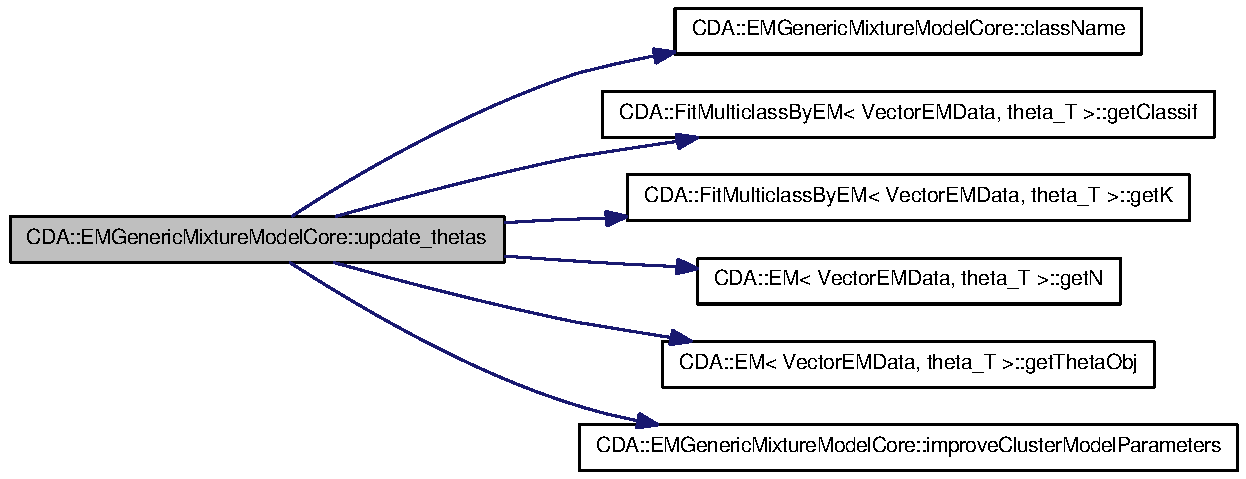
\includegraphics[width=317pt]{classCDA_1_1EMGenericMixtureModelCore_a12c68e86652d9a723ca0716f7676b360_cgraph}
\end{center}
\end{figure}




\subsection{Dokumentation der Datenelemente}
\hypertarget{classCDA_1_1EMGenericMixtureModelCore_ac31ee51281c9984de28e57351758a1a4}{
\index{CDA::EMGenericMixtureModelCore@{CDA::EMGenericMixtureModelCore}!P@{P}}
\index{P@{P}!CDA::EMGenericMixtureModelCore@{CDA::EMGenericMixtureModelCore}}
\subsubsection[{P}]{\setlength{\rightskip}{0pt plus 5cm}template$<$class theta\_\-T$>$ const unsigned {\bf CDA::EMGenericMixtureModelCore}$<$ theta\_\-T $>$::{\bf P}\hspace{0.3cm}{\ttfamily  \mbox{[}protected\mbox{]}}}}
\label{classCDA_1_1EMGenericMixtureModelCore_ac31ee51281c9984de28e57351758a1a4}


Parameter space dimensionality. 

\hypertarget{classCDA_1_1GaussianMixtureModelNDParams_NOTA}{}\subsection{BENE}\label{classCDA_1_1GaussianMixtureModelNDParams_NOTA}
We didn't count the class probability before, as it was handled differently. ONCE AND FOR ALL (but not for all times), P is counted INCLUDING the class prior probability. 

Die Dokumentation für diese Klasse wurde erzeugt aufgrund der Dateien:\begin{DoxyCompactItemize}
\item 
include/expmax/\hyperlink{EMGenericMixtureModelCore_8h_09_09}{EMGenericMixtureModelCore.h++}\item 
src/expmax/\hyperlink{EMGenericMixtureModelCore_8c_09_09}{EMGenericMixtureModelCore.c++}\end{DoxyCompactItemize}

\hypertarget{classCDA_1_1EMThetas}{
\section{CDA::EMThetas Klassenreferenz}
\label{classCDA_1_1EMThetas}\index{CDA::EMThetas@{CDA::EMThetas}}
}


Model parameters for \hyperlink{classCDA_1_1EM}{EM}.  




{\ttfamily \#include $<$EMTheta.h++$>$}



Basisklasse für \hyperlink{classCDA_1_1GaussianMixtureModelNDParams}{CDA::GaussianMixtureModelNDParams}.

\subsection*{Öffentliche Typen}
\begin{DoxyCompactItemize}
\item 
\hypertarget{classCDA_1_1EMThetas_aba47b3e7d71ea344695798e68471cc69}{
typedef fvector\_\-t \hyperlink{classCDA_1_1EMThetas_aba47b3e7d71ea344695798e68471cc69}{value\_\-type}}
\label{classCDA_1_1EMThetas_aba47b3e7d71ea344695798e68471cc69}

\begin{DoxyCompactList}\small\item\em Basic TYpedef. \item\end{DoxyCompactList}\end{DoxyCompactItemize}
\subsection*{Öffentliche Methoden}
\begin{DoxyCompactItemize}
\item 
\hyperlink{classCDA_1_1EMThetas_a97b7888efc058416d40ab7a24c80a2a0}{EMThetas} ()
\item 
\hyperlink{classCDA_1_1EMThetas_aaa3c2d20ee5d95a8b38d40e7c6d0b1a7}{EMThetas} (const \hyperlink{classCDA_1_1EMThetas}{EMThetas} \&other)
\item 
{\footnotesize template$<$class II $>$ }\\void \hyperlink{classCDA_1_1EMThetas_a1c8058269e4d8a32a2dd58f13ad94369}{setTheta} (std::pair$<$ II, II $>$ thetas\_\-)
\begin{DoxyCompactList}\small\item\em Initial guess for model parameters -\/-\/ strictly needed. \item\end{DoxyCompactList}\item 
\hypertarget{classCDA_1_1EMThetas_aadd9127ef459eda6eb890e1f3bd5a1bc}{
const std::vector$<$ fvector\_\-t $>$ \& \hyperlink{classCDA_1_1EMThetas_aadd9127ef459eda6eb890e1f3bd5a1bc}{getThetas} () const }
\label{classCDA_1_1EMThetas_aadd9127ef459eda6eb890e1f3bd5a1bc}

\begin{DoxyCompactList}\small\item\em const getter for normal access \item\end{DoxyCompactList}\item 
\hypertarget{classCDA_1_1EMThetas_a0d5cc0f815c7a78a42d2d64b2fd5bfdb}{
double \hyperlink{classCDA_1_1EMThetas_a0d5cc0f815c7a78a42d2d64b2fd5bfdb}{getThetas} (unsigned int k, unsigned int n) const }
\label{classCDA_1_1EMThetas_a0d5cc0f815c7a78a42d2d64b2fd5bfdb}

\begin{DoxyCompactList}\small\item\em const getter for normal access \item\end{DoxyCompactList}\item 
\hypertarget{classCDA_1_1EMThetas_ab5cc3d05862d41aa16a38b7c4ec51bd3}{
std::vector$<$ fvector\_\-t $>$ \& \hyperlink{classCDA_1_1EMThetas_ab5cc3d05862d41aa16a38b7c4ec51bd3}{getModifyThetas} ()}
\label{classCDA_1_1EMThetas_ab5cc3d05862d41aa16a38b7c4ec51bd3}

\begin{DoxyCompactList}\small\item\em non-\/const getter for updates only. \item\end{DoxyCompactList}\item 
\hypertarget{classCDA_1_1EMThetas_acc1246f42ca1fa55d8f7d1338dee39ef}{
fvector\_\-t::value\_\-type \& \hyperlink{classCDA_1_1EMThetas_acc1246f42ca1fa55d8f7d1338dee39ef}{getModifyThetas} (const unsigned k, const unsigned i)}
\label{classCDA_1_1EMThetas_acc1246f42ca1fa55d8f7d1338dee39ef}

\begin{DoxyCompactList}\small\item\em Important. \item\end{DoxyCompactList}\item 
unsigned int \hyperlink{classCDA_1_1EMThetas_aeafa1d8926150ea06a4f76228817d38e}{getP} () const 
\end{DoxyCompactItemize}
\subsection*{Geschützte Attribute}
\begin{DoxyCompactItemize}
\item 
\hypertarget{classCDA_1_1EMThetas_a2fb1c00c889f9a5bfe95e65ba1c4b132}{
std::vector$<$ fvector\_\-t $>$ \hyperlink{classCDA_1_1EMThetas_a2fb1c00c889f9a5bfe95e65ba1c4b132}{thetas}}
\label{classCDA_1_1EMThetas_a2fb1c00c889f9a5bfe95e65ba1c4b132}

\begin{DoxyCompactList}\small\item\em Model parameters possibly a single vector, or K PDF parameter vectors, one per class =$>$ these belong in the concrete classes? I hate duplication! \item\end{DoxyCompactList}\end{DoxyCompactItemize}


\subsection{Ausführliche Beschreibung}
Model parameters for \hyperlink{classCDA_1_1EM}{EM}. \hypertarget{ProbabilisticClustering_8h_09_09_DESCRIPTION}{}\subsection{DESCRIPTION}\label{ProbabilisticClustering_8h_09_09_DESCRIPTION}
To avoid duplication. Can't just put it into \hyperlink{classCDA_1_1EM}{EM} and inherit because of duplicate class problems\hypertarget{classCDA_1_1EMThetas_ARCHITECTURE}{}\subsection{CAVEAT}\label{classCDA_1_1EMThetas_ARCHITECTURE}
I dislike having this class around\hypertarget{classCDA_1_1EMThetas_ANYWAY}{}\subsection{ANYWAY}\label{classCDA_1_1EMThetas_ANYWAY}
TODO it should be possible to subclass this an handle all the parameter management (i.e. extraction of the right fields, some calculations) in here. 

\subsection{Beschreibung der Konstruktoren und Destruktoren}
\hypertarget{classCDA_1_1EMThetas_a97b7888efc058416d40ab7a24c80a2a0}{
\index{CDA::EMThetas@{CDA::EMThetas}!EMThetas@{EMThetas}}
\index{EMThetas@{EMThetas}!CDA::EMThetas@{CDA::EMThetas}}
\subsubsection[{EMThetas}]{\setlength{\rightskip}{0pt plus 5cm}EMThetas::EMThetas ()}}
\label{classCDA_1_1EMThetas_a97b7888efc058416d40ab7a24c80a2a0}
\hyperlink{classCDA_1_1EMThetas}{EMThetas} initialize empty \hypertarget{classCDA_1_1EMThetas_aaa3c2d20ee5d95a8b38d40e7c6d0b1a7}{
\index{CDA::EMThetas@{CDA::EMThetas}!EMThetas@{EMThetas}}
\index{EMThetas@{EMThetas}!CDA::EMThetas@{CDA::EMThetas}}
\subsubsection[{EMThetas}]{\setlength{\rightskip}{0pt plus 5cm}EMThetas::EMThetas (const {\bf EMThetas} \& {\em other})}}
\label{classCDA_1_1EMThetas_aaa3c2d20ee5d95a8b38d40e7c6d0b1a7}
\hyperlink{classCDA_1_1EMThetas}{EMThetas} copy constructor 

\subsection{Dokumentation der Elementfunktionen}
\hypertarget{classCDA_1_1EMThetas_aeafa1d8926150ea06a4f76228817d38e}{
\index{CDA::EMThetas@{CDA::EMThetas}!getP@{getP}}
\index{getP@{getP}!CDA::EMThetas@{CDA::EMThetas}}
\subsubsection[{getP}]{\setlength{\rightskip}{0pt plus 5cm}unsigned int CDA::EMThetas::getP () const\hspace{0.3cm}{\ttfamily  \mbox{[}inline\mbox{]}}}}
\label{classCDA_1_1EMThetas_aeafa1d8926150ea06a4f76228817d38e}
\begin{Desc}
\item[\hyperlink{todo__todo000004}{Noch zu erledigen}]TODO umHimmels Willen! \end{Desc}


Erneute Implementation in \hyperlink{classCDA_1_1GaussianMixtureModelNDParams_a381c2e9b2f537dfb8558d202a9cb12ea}{CDA::GaussianMixtureModelNDParams}.

\hypertarget{classCDA_1_1EMThetas_a1c8058269e4d8a32a2dd58f13ad94369}{
\index{CDA::EMThetas@{CDA::EMThetas}!setTheta@{setTheta}}
\index{setTheta@{setTheta}!CDA::EMThetas@{CDA::EMThetas}}
\subsubsection[{setTheta}]{\setlength{\rightskip}{0pt plus 5cm}template$<$class II $>$ void CDA::EMThetas::setTheta (std::pair$<$ II, II $>$ {\em thetas\_\-})\hspace{0.3cm}{\ttfamily  \mbox{[}inline\mbox{]}}}}
\label{classCDA_1_1EMThetas_a1c8058269e4d8a32a2dd58f13ad94369}


Initial guess for model parameters -\/-\/ strictly needed. 

\hypertarget{classCDA_1_1EMThetas_CAREFUL}{}\subsection{CAREFUL}\label{classCDA_1_1EMThetas_CAREFUL}
Input data format differs for each individual distribution, be careful and read the documentation. =$>$ will be solved by {\bfseries subclassing} and creating specific setters/getters

\begin{Desc}
\item[\hyperlink{todo__todo000003}{Noch zu erledigen}]random numbers or something when none given \end{Desc}


Die Dokumentation für diese Klasse wurde erzeugt aufgrund der Dateien:\begin{DoxyCompactItemize}
\item 
include/expmax/\hyperlink{EMTheta_8h_09_09}{EMTheta.h++}\item 
src/expmax/\hyperlink{EMTheta_8c_09_09}{EMTheta.c++}\end{DoxyCompactItemize}

\hypertarget{classCDA_1_1EnhancedDataset}{
\section{CDA::EnhancedDataset Klassenreferenz}
\label{classCDA_1_1EnhancedDataset}\index{CDA::EnhancedDataset@{CDA::EnhancedDataset}}
}


aware of basic statistics for normalization etc.  




{\ttfamily \#include $<$Data.h++$>$}

\subsection*{Öffentliche Typen}
\begin{DoxyCompactItemize}
\item 
\hypertarget{classCDA_1_1EnhancedDataset_ac48f706bc85385da7b78ff9229666475}{
typedef std::vector$<$ fvector\_\-t $>$ {\bfseries dataframe\_\-t}}
\label{classCDA_1_1EnhancedDataset_ac48f706bc85385da7b78ff9229666475}

\item 
\hypertarget{classCDA_1_1EnhancedDataset_ad01be5e014bc9a5232102fae6759caad}{
typedef fvector\_\-t {\bfseries row\_\-t}}
\label{classCDA_1_1EnhancedDataset_ad01be5e014bc9a5232102fae6759caad}

\item 
\hypertarget{classCDA_1_1EnhancedDataset_ad125a62150f81238cd207baaa057b4ff}{
typedef accumulator\_\-set$<$ double, stats$<$ tag::mean, tag::variance, tag::max, tag::min $>$ $>$ {\bfseries boost\_\-statistics\_\-t}}
\label{classCDA_1_1EnhancedDataset_ad125a62150f81238cd207baaa057b4ff}

\item 
\hypertarget{classCDA_1_1EnhancedDataset_adecd4f314f8fc01ba75b08ca053ba561}{
typedef boost::transform\_\-iterator$<$ boost::function$<$ const fvector\_\-t \&(const fvector\_\-t \&)$>$, dataframe\_\-t::const\_\-iterator $>$ {\bfseries vtrit\_\-t}}
\label{classCDA_1_1EnhancedDataset_adecd4f314f8fc01ba75b08ca053ba561}

\end{DoxyCompactItemize}
\subsection*{Öffentliche Methoden}
\begin{DoxyCompactItemize}
\item 
\hypertarget{classCDA_1_1EnhancedDataset_a38188f6537aecfdb93351da5d0814b4a}{
{\bfseries EnhancedDataset} (unsigned D\_\-)}
\label{classCDA_1_1EnhancedDataset_a38188f6537aecfdb93351da5d0814b4a}

\item 
\hypertarget{classCDA_1_1EnhancedDataset_a396c10698c80b47cd23be67c95dce5d4}{
void {\bfseries addRow} (const fvector\_\-t \&datarow)}
\label{classCDA_1_1EnhancedDataset_a396c10698c80b47cd23be67c95dce5d4}

\item 
\hypertarget{classCDA_1_1EnhancedDataset_abb24dc80e0c2f2e6c2031e4093d6a460}{
const dataframe\_\-t \& {\bfseries getData} () const }
\label{classCDA_1_1EnhancedDataset_abb24dc80e0c2f2e6c2031e4093d6a460}

\item 
\hypertarget{classCDA_1_1EnhancedDataset_aa15349d7a7c21254a2aeb529fba1ecb3}{
size\_\-t {\bfseries N} () const }
\label{classCDA_1_1EnhancedDataset_aa15349d7a7c21254a2aeb529fba1ecb3}

\item 
\hypertarget{classCDA_1_1EnhancedDataset_a922889380d5f8ea30102266a0d1e7a7e}{
{\footnotesize template$<$class boost\_\-accumtag $>$ }\\fvector\_\-t {\bfseries getStatistics} () const }
\label{classCDA_1_1EnhancedDataset_a922889380d5f8ea30102266a0d1e7a7e}

\item 
\hypertarget{classCDA_1_1EnhancedDataset_a664e728858339f8729a5c154d3dbe519}{
double \hyperlink{classCDA_1_1EnhancedDataset_a664e728858339f8729a5c154d3dbe519}{getMinOfAny} () const }
\label{classCDA_1_1EnhancedDataset_a664e728858339f8729a5c154d3dbe519}

\begin{DoxyCompactList}\small\item\em Handy for quick normalization, all dimensions scaled by same factor. \item\end{DoxyCompactList}\item 
\hypertarget{classCDA_1_1EnhancedDataset_a7d063419540f0da32bf6a242e9c0b513}{
double \hyperlink{classCDA_1_1EnhancedDataset_a7d063419540f0da32bf6a242e9c0b513}{getMaxOfAny} () const }
\label{classCDA_1_1EnhancedDataset_a7d063419540f0da32bf6a242e9c0b513}

\begin{DoxyCompactList}\small\item\em Handy for quick normalization, all dimensions scaled by same factor. \item\end{DoxyCompactList}\item 
\hypertarget{classCDA_1_1EnhancedDataset_af3fa7167971e2ac2eda248c849de722d}{
fvector\_\-t {\bfseries getNormalized} (unsigned idx) const }
\label{classCDA_1_1EnhancedDataset_af3fa7167971e2ac2eda248c849de722d}

\item 
\hypertarget{classCDA_1_1EnhancedDataset_a6e5b4a6f8a8a220aed9fbc6c834e0b38}{
const fvector\_\-t \& {\bfseries normalize} (const fvector\_\-t \&in) const }
\label{classCDA_1_1EnhancedDataset_a6e5b4a6f8a8a220aed9fbc6c834e0b38}

\item 
\hypertarget{classCDA_1_1EnhancedDataset_a781f6fe7714713bb70ad6a50b9b08731}{
{\footnotesize template$<$class indexcoll\_\-t $>$ }\\fvector\_\-t {\bfseries normalize\_\-selective} (const fvector\_\-t \&in, indexcoll\_\-t \&slc) const }
\label{classCDA_1_1EnhancedDataset_a781f6fe7714713bb70ad6a50b9b08731}

\item 
\hypertarget{classCDA_1_1EnhancedDataset_a683ee6b03fc4ce6766d45cb05d5cb855}{
{\footnotesize template$<$class indexcoll\_\-t $>$ }\\boost::shared\_\-ptr$<$ \hyperlink{classCDA_1_1EnhancedDataset}{EnhancedDataset} $>$ \hyperlink{classCDA_1_1EnhancedDataset_a683ee6b03fc4ce6766d45cb05d5cb855}{normalized} (indexcoll\_\-t \&slc) const }
\label{classCDA_1_1EnhancedDataset_a683ee6b03fc4ce6766d45cb05d5cb855}

\begin{DoxyCompactList}\small\item\em Normalize only the selected fields. \item\end{DoxyCompactList}\item 
\hypertarget{classCDA_1_1EnhancedDataset_a6159b71320f3e076639b72d202817c30}{
{\footnotesize template$<$class indexcoll\_\-t $>$ }\\boost::shared\_\-ptr$<$ \hyperlink{classCDA_1_1EnhancedDataset}{EnhancedDataset} $>$ {\bfseries projected} (indexcoll\_\-t \&slc) const }
\label{classCDA_1_1EnhancedDataset_a6159b71320f3e076639b72d202817c30}

\item 
\hypertarget{classCDA_1_1EnhancedDataset_a27f451c43eb9ca54b10b2463047af559}{
std::pair$<$ vtrit\_\-t, vtrit\_\-t $>$ {\bfseries getNormalizedIterPair} () const }
\label{classCDA_1_1EnhancedDataset_a27f451c43eb9ca54b10b2463047af559}

\item 
\hypertarget{classCDA_1_1EnhancedDataset_a7545c4c91dff1ccea71b02b5acdba507}{
std::pair$<$ dataframe\_\-t::const\_\-iterator, dataframe\_\-t::const\_\-iterator $>$ {\bfseries getIterPair} () const }
\label{classCDA_1_1EnhancedDataset_a7545c4c91dff1ccea71b02b5acdba507}

\item 
\hypertarget{classCDA_1_1EnhancedDataset_a52334e7e5f1fb68e0414a42cbb4a6d6d}{
{\footnotesize template$<$class F $>$ }\\std::pair$<$ boost::filter\_\-iterator$<$ F, dataframe\_\-t::const\_\-iterator $>$, boost::filter\_\-iterator$<$ F, dataframe\_\-t::const\_\-iterator $>$ $>$ {\bfseries getFilteredIterPair} (F \&function) const }
\label{classCDA_1_1EnhancedDataset_a52334e7e5f1fb68e0414a42cbb4a6d6d}

\end{DoxyCompactItemize}
\subsection*{Öffentliche Attribute}
\begin{DoxyCompactItemize}
\item 
\hypertarget{classCDA_1_1EnhancedDataset_a10e8496988b39465453b93894c1532d1}{
dataframe\_\-t {\bfseries m\_\-data}}
\label{classCDA_1_1EnhancedDataset_a10e8496988b39465453b93894c1532d1}

\item 
\hypertarget{classCDA_1_1EnhancedDataset_ae2e4868942ed33abf9d495b59525933b}{
unsigned {\bfseries D}}
\label{classCDA_1_1EnhancedDataset_ae2e4868942ed33abf9d495b59525933b}

\item 
\hypertarget{classCDA_1_1EnhancedDataset_a0a2a1d4c3eda234c49cc8192b5924045}{
std::vector$<$ boost\_\-statistics\_\-t $>$ \hyperlink{classCDA_1_1EnhancedDataset_a0a2a1d4c3eda234c49cc8192b5924045}{accs}}
\label{classCDA_1_1EnhancedDataset_a0a2a1d4c3eda234c49cc8192b5924045}

\begin{DoxyCompactList}\small\item\em One for each dimension. \item\end{DoxyCompactList}\end{DoxyCompactItemize}


\subsection{Ausführliche Beschreibung}
aware of basic statistics for normalization etc. 

Die Dokumentation für diese Klasse wurde erzeugt aufgrund der Datei:\begin{DoxyCompactItemize}
\item 
include/data/\hyperlink{Data_8h_09_09}{Data.h++}\end{DoxyCompactItemize}

\hypertarget{classCDA_1_1EnhancedDatasetView}{
\section{CDA::EnhancedDatasetView Klassenreferenz}
\label{classCDA_1_1EnhancedDatasetView}\index{CDA::EnhancedDatasetView@{CDA::EnhancedDatasetView}}
}


Die Dokumentation für diese Klasse wurde erzeugt aufgrund der Datei:\begin{DoxyCompactItemize}
\item 
include/data/\hyperlink{Data_8h_09_09}{Data.h++}\end{DoxyCompactItemize}

\hypertarget{classCDA_1_1FitMulticlassByEM}{
\section{CDA::FitMulticlassByEM$<$ data\_\-T, theta\_\-T $>$ Template-\/Klassenreferenz}
\label{classCDA_1_1FitMulticlassByEM}\index{CDA::FitMulticlassByEM@{CDA::FitMulticlassByEM}}
}


An abstract model fitting class The next after \hyperlink{classCDA_1_1EM}{EM} class ...  




{\ttfamily \#include $<$FitMulticlassByEM.h++$>$}



Abgeleitet von \hyperlink{classCDA_1_1EM}{CDA::EM$<$ data\_\-T, theta\_\-T $>$}.



Zusammengehörigkeiten von CDA::FitMulticlassByEM$<$ data\_\-T, theta\_\-T $>$:\nopagebreak
\begin{figure}[H]
\begin{center}
\leavevmode
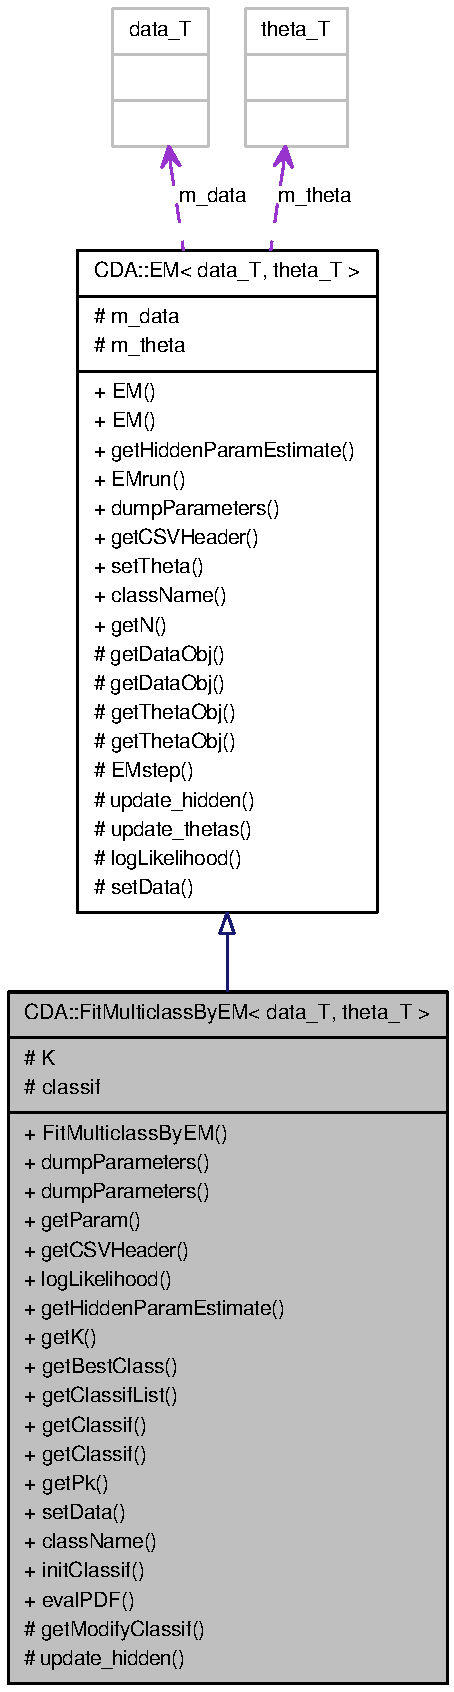
\includegraphics[height=400pt]{classCDA_1_1FitMulticlassByEM__coll__graph}
\end{center}
\end{figure}
\subsection*{Öffentliche Typen}
\begin{DoxyCompactItemize}
\item 
\hypertarget{classCDA_1_1FitMulticlassByEM_a05aa6cf01041a71df27a4b8be40298ba}{
typedef data\_\-T \hyperlink{classCDA_1_1FitMulticlassByEM_a05aa6cf01041a71df27a4b8be40298ba}{data\_\-t}}
\label{classCDA_1_1FitMulticlassByEM_a05aa6cf01041a71df27a4b8be40298ba}

\begin{DoxyCompactList}\small\item\em Propagate the datapoint\_\-t etc. Why can't we give it the same name? Annoying. \item\end{DoxyCompactList}\item 
\hypertarget{classCDA_1_1FitMulticlassByEM_a3ddfc994fa8e2960feb82e5e6a4103b2}{
typedef data\_\-T::value\_\-type {\bfseries datapoint\_\-t}}
\label{classCDA_1_1FitMulticlassByEM_a3ddfc994fa8e2960feb82e5e6a4103b2}

\item 
\hypertarget{classCDA_1_1FitMulticlassByEM_afc23366fb0906a43ae74e0b7c9b26db4}{
typedef theta\_\-T {\bfseries theta\_\-t}}
\label{classCDA_1_1FitMulticlassByEM_afc23366fb0906a43ae74e0b7c9b26db4}

\end{DoxyCompactItemize}
\subsection*{Öffentliche Methoden}
\begin{DoxyCompactItemize}
\item 
\hyperlink{classCDA_1_1FitMulticlassByEM_a42ba3e452dfee55767219ab9571b0dd5}{FitMulticlassByEM} (const unsigned K\_\-, const \hyperlink{classCDA_1_1FitMulticlassByEM_a05aa6cf01041a71df27a4b8be40298ba}{data\_\-t} \&data, const theta\_\-t \&theta)
\item 
const std::string \hyperlink{classCDA_1_1FitMulticlassByEM_aa5598f1ced5c95045f59c99610ab53e5}{dumpParameters} (const unsigned k, const boost::optional$<$ unsigned int $>$ iteration) const 
\begin{DoxyCompactList}\small\item\em Output CSV. \item\end{DoxyCompactList}\item 
const std::string \hyperlink{classCDA_1_1FitMulticlassByEM_abd04a7135250a427a100c95bf2bf43a9}{dumpParameters} (const boost::optional$<$ unsigned int $>$ iteration) const 
\begin{DoxyCompactList}\small\item\em Output CSV. \item\end{DoxyCompactList}\item 
double \hyperlink{classCDA_1_1FitMulticlassByEM_a4185d0f323087ef9112e903a2782fdfd}{getParam} (const unsigned k, const unsigned p) const 
\begin{DoxyCompactList}\small\item\em Conveniently encapsulate access ofm\_\-theta. \item\end{DoxyCompactList}\item 
\hypertarget{classCDA_1_1FitMulticlassByEM_aec99fc55d806d855e02b9a2fc96887a0}{
virtual const std::string \hyperlink{classCDA_1_1FitMulticlassByEM_aec99fc55d806d855e02b9a2fc96887a0}{getCSVHeader} () const =0}
\label{classCDA_1_1FitMulticlassByEM_aec99fc55d806d855e02b9a2fc96887a0}

\begin{DoxyCompactList}\small\item\em Header to go with the CSV output. Must be reimplemented. \item\end{DoxyCompactList}\item 
double \hyperlink{classCDA_1_1FitMulticlassByEM_abaea206aef382360246cf2a64dadc74c}{logLikelihood} () const 
\begin{DoxyCompactList}\small\item\em Implemented here. \item\end{DoxyCompactList}\item 
const fvector\_\-t \& \hyperlink{classCDA_1_1FitMulticlassByEM_ae5a9232f142123c9ffaf6ec956b44f00}{getHiddenParamEstimate} (const unsigned n) const 
\begin{DoxyCompactList}\small\item\em Getter for estimate. \item\end{DoxyCompactList}\item 
\hypertarget{classCDA_1_1FitMulticlassByEM_ae6b0acc500e8360bee6f8e3434b6b197}{
unsigned int \hyperlink{classCDA_1_1FitMulticlassByEM_ae6b0acc500e8360bee6f8e3434b6b197}{getK} () const }
\label{classCDA_1_1FitMulticlassByEM_ae6b0acc500e8360bee6f8e3434b6b197}

\begin{DoxyCompactList}\small\item\em Better have a getter for this too. \item\end{DoxyCompactList}\item 
unsigned int \hyperlink{classCDA_1_1FitMulticlassByEM_a60164ed52d11dc10b4faee5de96d42a7}{getBestClass} (const unsigned n) const 
\begin{DoxyCompactList}\small\item\em Get class with best estimated membership probability. \item\end{DoxyCompactList}\item 
std::vector$<$ unsigned int $>$ \hyperlink{classCDA_1_1FitMulticlassByEM_a915e6a0aaae5f74c5802b53fbed8278a}{getClassifList} () const 
\begin{DoxyCompactList}\small\item\em Read classification results (1). \item\end{DoxyCompactList}\item 
const std::vector$<$ fvector\_\-t $>$ \& \hyperlink{classCDA_1_1FitMulticlassByEM_ad468afb0c45474a7400fd7efbb1ad2dd}{getClassif} () const 
\item 
const fvector\_\-t \& \hyperlink{classCDA_1_1FitMulticlassByEM_addcc14007ec1f00046391c3ac7572e34}{getClassif} (const unsigned n) const 
\item 
double \hyperlink{classCDA_1_1FitMulticlassByEM_a869530b76ee4b40d38d3fb80ea0932aa}{getPk} (const unsigned k) const 
\begin{DoxyCompactList}\small\item\em Get current estimated class weight. \item\end{DoxyCompactList}\item 
\hypertarget{classCDA_1_1FitMulticlassByEM_a7247bfcad3c828f9cf372b6c414e93f0}{
{\footnotesize template$<$class II $>$ }\\void \hyperlink{classCDA_1_1FitMulticlassByEM_a7247bfcad3c828f9cf372b6c414e93f0}{setData} (std::pair$<$ II, II $>$ data\_\-)}
\label{classCDA_1_1FitMulticlassByEM_a7247bfcad3c828f9cf372b6c414e93f0}

\begin{DoxyCompactList}\small\item\em Initialize known samples, i.e. your data points Also initialize the classif vector. \item\end{DoxyCompactList}\item 
virtual const std::string \hyperlink{classCDA_1_1FitMulticlassByEM_a885947f2c93b4a05cb3eb153d774cb75}{className} () const 
\item 
void \hyperlink{classCDA_1_1FitMulticlassByEM_aceb43b0a386c8f8e112562cc3288b23d}{initClassif} ()
\begin{DoxyCompactList}\small\item\em Initialize class membership beliefs. \item\end{DoxyCompactList}\item 
virtual double \hyperlink{classCDA_1_1FitMulticlassByEM_a747d8926ab25896e4a5db08b169fccde}{evalPDF} (const unsigned k, const datapoint\_\-t \&x) const =0
\begin{DoxyCompactList}\small\item\em Evaluate the cluster model PDF with class parameters $k$ at $\vec{x}$. \item\end{DoxyCompactList}\end{DoxyCompactItemize}
\subsection*{Geschützte Methoden}
\begin{DoxyCompactItemize}
\item 
std::vector$<$ fvector\_\-t $>$ \& \hyperlink{classCDA_1_1FitMulticlassByEM_a07c7f0fb577bb28b7987e80bb93d6707}{getModifyClassif} ()
\item 
void \hyperlink{classCDA_1_1FitMulticlassByEM_a7c40c5528a4b8b32e2455056f60d76de}{update\_\-hidden} ()
\begin{DoxyCompactList}\small\item\em {\bfseries E-\/step}: update hidden attributes, i.e. classification \item\end{DoxyCompactList}\end{DoxyCompactItemize}
\subsection*{Geschützte Attribute}
\begin{DoxyCompactItemize}
\item 
\hypertarget{classCDA_1_1FitMulticlassByEM_a315d727c0edf745ae12f63a20db0e79e}{
const unsigned \hyperlink{classCDA_1_1FitMulticlassByEM_a315d727c0edf745ae12f63a20db0e79e}{K}}
\label{classCDA_1_1FitMulticlassByEM_a315d727c0edf745ae12f63a20db0e79e}

\begin{DoxyCompactList}\small\item\em Number of individual Distributions. \item\end{DoxyCompactList}\item 
\hypertarget{classCDA_1_1FitMulticlassByEM_aebd80b2bdf01b62d279023cfb50cf3e6}{
std::vector$<$ fvector\_\-t $>$ \hyperlink{classCDA_1_1FitMulticlassByEM_aebd80b2bdf01b62d279023cfb50cf3e6}{classif}}
\label{classCDA_1_1FitMulticlassByEM_aebd80b2bdf01b62d279023cfb50cf3e6}

\begin{DoxyCompactList}\small\item\em N classes: class appartenance probabilities. \item\end{DoxyCompactList}\end{DoxyCompactItemize}


\subsection{Ausführliche Beschreibung}
\subsubsection*{template$<$class data\_\-T, class theta\_\-T$>$ class CDA::FitMulticlassByEM$<$ data\_\-T, theta\_\-T $>$}

An abstract model fitting class The next after \hyperlink{classCDA_1_1EM}{EM} class ... 
\begin{DoxyTemplParams}{Template Parameters}
\item[{\em }]the datapoint\_\-t (fvector\_\-t or double .. or anything!) \end{DoxyTemplParams}


\subsection{Beschreibung der Konstruktoren und Destruktoren}
\hypertarget{classCDA_1_1FitMulticlassByEM_a42ba3e452dfee55767219ab9571b0dd5}{
\index{CDA::FitMulticlassByEM@{CDA::FitMulticlassByEM}!FitMulticlassByEM@{FitMulticlassByEM}}
\index{FitMulticlassByEM@{FitMulticlassByEM}!CDA::FitMulticlassByEM@{CDA::FitMulticlassByEM}}
\subsubsection[{FitMulticlassByEM}]{\setlength{\rightskip}{0pt plus 5cm}template$<$class data\_\-T, class theta\_\-T$>$ {\bf CDA::FitMulticlassByEM}$<$ data\_\-T, theta\_\-T $>$::{\bf FitMulticlassByEM} (const unsigned {\em K\_\-}, \/  const {\bf data\_\-t} \& {\em data}, \/  const theta\_\-t \& {\em theta})\hspace{0.3cm}{\ttfamily  \mbox{[}inline\mbox{]}}}}
\label{classCDA_1_1FitMulticlassByEM_a42ba3e452dfee55767219ab9571b0dd5}
Constructor

To be called by subclasses


\begin{DoxyParams}{Parameter}
\item[\mbox{$\leftarrow$} {\em K\_\-}]Number of Classes ($\sim$) \item[\mbox{$\leftarrow$} {\em data}]\item[\mbox{$\leftarrow$} {\em theta}]\end{DoxyParams}


\subsection{Dokumentation der Elementfunktionen}
\hypertarget{classCDA_1_1FitMulticlassByEM_a885947f2c93b4a05cb3eb153d774cb75}{
\index{CDA::FitMulticlassByEM@{CDA::FitMulticlassByEM}!className@{className}}
\index{className@{className}!CDA::FitMulticlassByEM@{CDA::FitMulticlassByEM}}
\subsubsection[{className}]{\setlength{\rightskip}{0pt plus 5cm}template$<$class data\_\-T, class theta\_\-T$>$ virtual const std::string {\bf CDA::FitMulticlassByEM}$<$ data\_\-T, theta\_\-T $>$::className () const\hspace{0.3cm}{\ttfamily  \mbox{[}inline, virtual\mbox{]}}}}
\label{classCDA_1_1FitMulticlassByEM_a885947f2c93b4a05cb3eb153d774cb75}
I know, same ... bc of template params 

Erneute Implementation von \hyperlink{classCDA_1_1EM_aa3edb551271b47675c817fa6c302741d}{CDA::EM$<$ data\_\-T, theta\_\-T $>$}.



Erneute Implementation in \hyperlink{classCDA_1_1EMGenericMixtureModelCore_a6e444765b04615888d41c4ab6c82ae61}{CDA::EMGenericMixtureModelCore$<$ theta\_\-T $>$}, \hyperlink{classCDA_1_1GaussianMixtureModel_aec72323935694359e18e3363ceaa40e7}{CDA::GaussianMixtureModel}, \hyperlink{classCDA_1_1GaussianMixtureModel1D_a08a734c5b74bccda43429df49db58edf}{CDA::GaussianMixtureModel1D} und \hyperlink{classCDA_1_1EMGenericMixtureModelCore_a6e444765b04615888d41c4ab6c82ae61}{CDA::EMGenericMixtureModelCore$<$ GaussianMixtureModelNDParams $>$}.



Hier ist ein Graph der zeigt, wo diese Funktion aufgerufen wird:\nopagebreak
\begin{figure}[H]
\begin{center}
\leavevmode
\includegraphics[width=227pt]{classCDA_1_1FitMulticlassByEM_a885947f2c93b4a05cb3eb153d774cb75_icgraph}
\end{center}
\end{figure}


\hypertarget{classCDA_1_1FitMulticlassByEM_abd04a7135250a427a100c95bf2bf43a9}{
\index{CDA::FitMulticlassByEM@{CDA::FitMulticlassByEM}!dumpParameters@{dumpParameters}}
\index{dumpParameters@{dumpParameters}!CDA::FitMulticlassByEM@{CDA::FitMulticlassByEM}}
\subsubsection[{dumpParameters}]{\setlength{\rightskip}{0pt plus 5cm}template$<$class data\_\-T , class theta\_\-T $>$ const std::string FitMulticlassByEM::dumpParameters (const boost::optional$<$ unsigned int $>$ {\em iteration}) const\hspace{0.3cm}{\ttfamily  \mbox{[}inline, virtual\mbox{]}}}}
\label{classCDA_1_1FitMulticlassByEM_abd04a7135250a427a100c95bf2bf43a9}


Output CSV. 


\begin{DoxyParams}{Parameter}
\item[\mbox{$\leftarrow$} {\em iteration}](optional) output iteration no. in first column\end{DoxyParams}
\begin{DoxyReturn}{Rückgabe}
multiple CSV lines 
\end{DoxyReturn}


Implementiert \hyperlink{classCDA_1_1EM_ad2deb0f1d94dc57a6e431caebeb34cbe}{CDA::EM$<$ data\_\-T, theta\_\-T $>$}.



Hier ist ein Graph der zeigt, was diese Funktion aufruft:\nopagebreak
\begin{figure}[H]
\begin{center}
\leavevmode
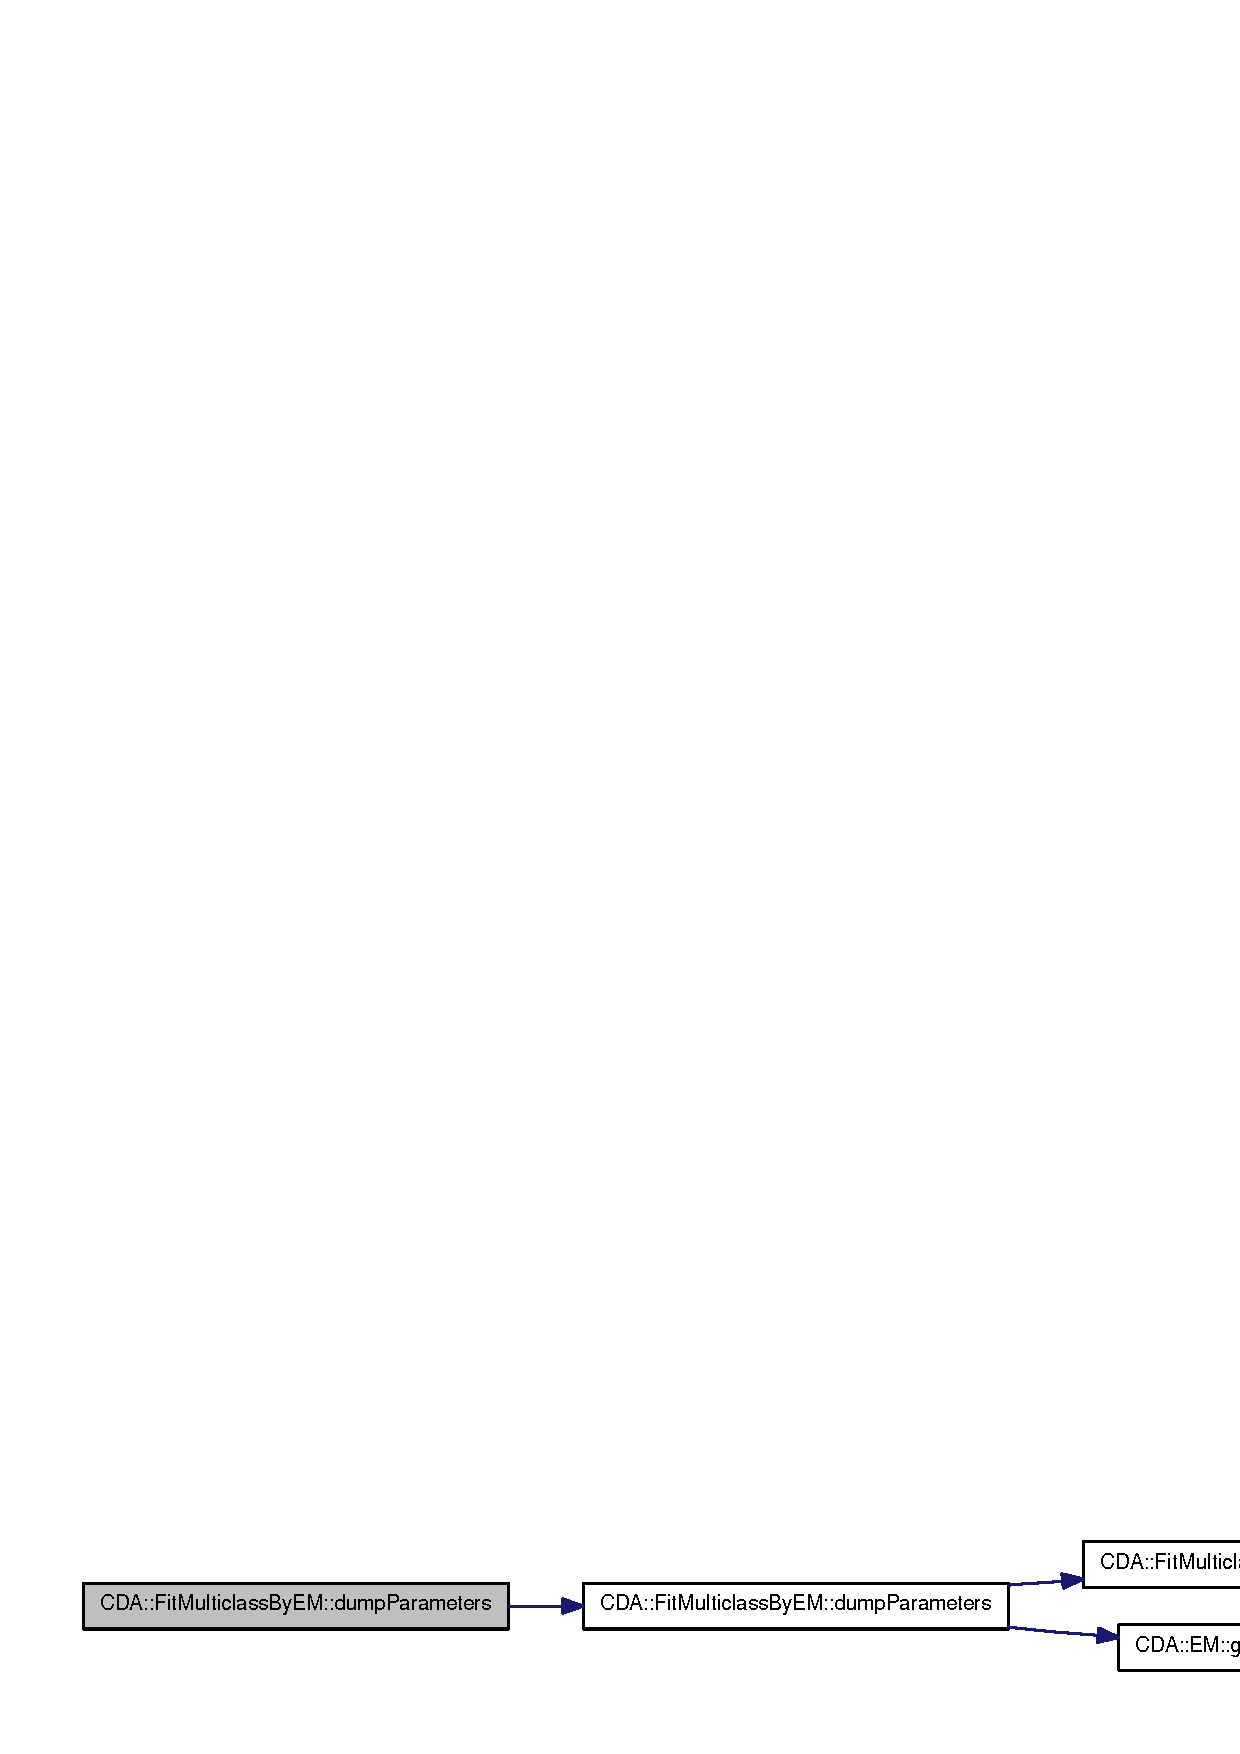
\includegraphics[width=337pt]{classCDA_1_1FitMulticlassByEM_abd04a7135250a427a100c95bf2bf43a9_cgraph}
\end{center}
\end{figure}


\hypertarget{classCDA_1_1FitMulticlassByEM_aa5598f1ced5c95045f59c99610ab53e5}{
\index{CDA::FitMulticlassByEM@{CDA::FitMulticlassByEM}!dumpParameters@{dumpParameters}}
\index{dumpParameters@{dumpParameters}!CDA::FitMulticlassByEM@{CDA::FitMulticlassByEM}}
\subsubsection[{dumpParameters}]{\setlength{\rightskip}{0pt plus 5cm}template$<$class data\_\-T , class theta\_\-T $>$ const std::string FitMulticlassByEM::dumpParameters (const unsigned {\em k}, \/  const boost::optional$<$ unsigned int $>$ {\em iteration}) const\hspace{0.3cm}{\ttfamily  \mbox{[}inline\mbox{]}}}}
\label{classCDA_1_1FitMulticlassByEM_aa5598f1ced5c95045f59c99610ab53e5}


Output CSV. 


\begin{DoxyParams}{Parameter}
\item[\mbox{$\leftarrow$} {\em k}]class \item[\mbox{$\leftarrow$} {\em iteration}](optional) output iteration no. in first column\end{DoxyParams}
\begin{DoxyReturn}{Rückgabe}
one CSV line 
\end{DoxyReturn}


Hier ist ein Graph der zeigt, was diese Funktion aufruft:\nopagebreak
\begin{figure}[H]
\begin{center}
\leavevmode
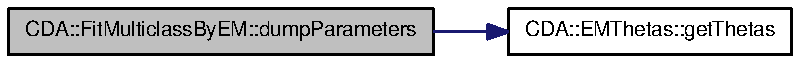
\includegraphics[width=217pt]{classCDA_1_1FitMulticlassByEM_aa5598f1ced5c95045f59c99610ab53e5_cgraph}
\end{center}
\end{figure}




Hier ist ein Graph der zeigt, wo diese Funktion aufgerufen wird:\nopagebreak
\begin{figure}[H]
\begin{center}
\leavevmode
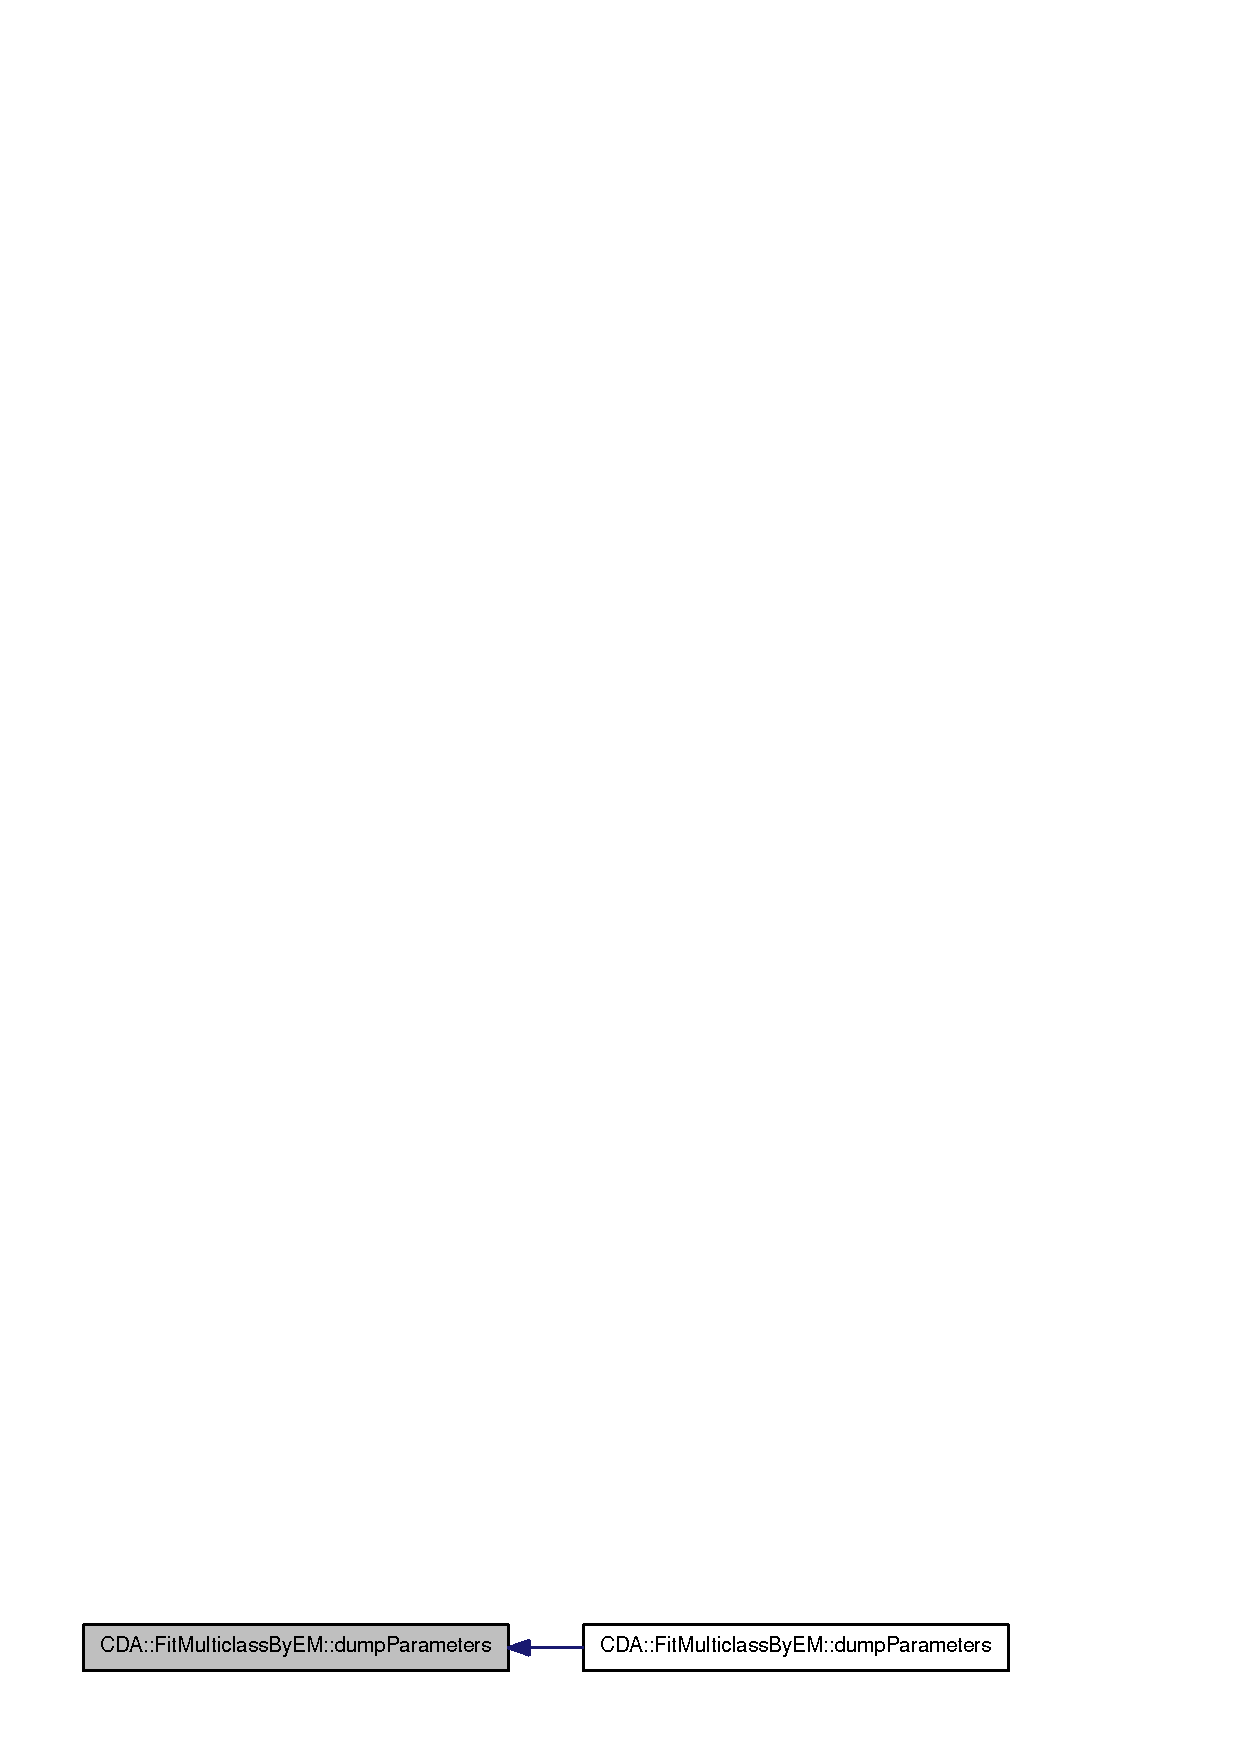
\includegraphics[width=244pt]{classCDA_1_1FitMulticlassByEM_aa5598f1ced5c95045f59c99610ab53e5_icgraph}
\end{center}
\end{figure}


\hypertarget{classCDA_1_1FitMulticlassByEM_a747d8926ab25896e4a5db08b169fccde}{
\index{CDA::FitMulticlassByEM@{CDA::FitMulticlassByEM}!evalPDF@{evalPDF}}
\index{evalPDF@{evalPDF}!CDA::FitMulticlassByEM@{CDA::FitMulticlassByEM}}
\subsubsection[{evalPDF}]{\setlength{\rightskip}{0pt plus 5cm}template$<$class data\_\-T, class theta\_\-T$>$ virtual double {\bf CDA::FitMulticlassByEM}$<$ data\_\-T, theta\_\-T $>$::evalPDF (const unsigned {\em k}, \/  const datapoint\_\-t \& {\em x}) const\hspace{0.3cm}{\ttfamily  \mbox{[}pure virtual\mbox{]}}}}
\label{classCDA_1_1FitMulticlassByEM_a747d8926ab25896e4a5db08b169fccde}


Evaluate the cluster model PDF with class parameters $k$ at $\vec{x}$. 


\begin{DoxyParams}{Parameter}
\item[\mbox{$\leftarrow$} {\em k}]class \item[\mbox{$\leftarrow$} {\em x}]feature vector\end{DoxyParams}
\begin{DoxyReturn}{Rückgabe}
probability $p(x,k\vert\theta)$ 
\end{DoxyReturn}


Implementiert in \hyperlink{classCDA_1_1GaussianMixtureModelNDCommon_aeac07962bd15c826561c68af7ac9c6d1}{CDA::GaussianMixtureModelNDCommon} und \hyperlink{classCDA_1_1EMGenericMixtureModelCore_ad8722983ea6f58d6e0b4a6bd117b050a}{CDA::EMGenericMixtureModelCore$<$ GaussianMixtureModelNDParams $>$}.



Hier ist ein Graph der zeigt, wo diese Funktion aufgerufen wird:\nopagebreak
\begin{figure}[H]
\begin{center}
\leavevmode
\includegraphics[width=221pt]{classCDA_1_1FitMulticlassByEM_a747d8926ab25896e4a5db08b169fccde_icgraph}
\end{center}
\end{figure}


\hypertarget{classCDA_1_1FitMulticlassByEM_a60164ed52d11dc10b4faee5de96d42a7}{
\index{CDA::FitMulticlassByEM@{CDA::FitMulticlassByEM}!getBestClass@{getBestClass}}
\index{getBestClass@{getBestClass}!CDA::FitMulticlassByEM@{CDA::FitMulticlassByEM}}
\subsubsection[{getBestClass}]{\setlength{\rightskip}{0pt plus 5cm}template$<$class data\_\-T , class theta\_\-T $>$ unsigned int FitMulticlassByEM::getBestClass (const unsigned {\em n}) const\hspace{0.3cm}{\ttfamily  \mbox{[}inline\mbox{]}}}}
\label{classCDA_1_1FitMulticlassByEM_a60164ed52d11dc10b4faee5de96d42a7}


Get class with best estimated membership probability. 


\begin{DoxyParams}{Parameter}
\item[\mbox{$\leftarrow$} {\em n}]Point number n \end{DoxyParams}


Hier ist ein Graph der zeigt, was diese Funktion aufruft:\nopagebreak
\begin{figure}[H]
\begin{center}
\leavevmode
\includegraphics[width=255pt]{classCDA_1_1FitMulticlassByEM_a60164ed52d11dc10b4faee5de96d42a7_cgraph}
\end{center}
\end{figure}


\hypertarget{classCDA_1_1FitMulticlassByEM_addcc14007ec1f00046391c3ac7572e34}{
\index{CDA::FitMulticlassByEM@{CDA::FitMulticlassByEM}!getClassif@{getClassif}}
\index{getClassif@{getClassif}!CDA::FitMulticlassByEM@{CDA::FitMulticlassByEM}}
\subsubsection[{getClassif}]{\setlength{\rightskip}{0pt plus 5cm}template$<$class data\_\-T , class theta\_\-T $>$ const fvector\_\-t \& FitMulticlassByEM::getClassif (const unsigned {\em n}) const\hspace{0.3cm}{\ttfamily  \mbox{[}inline\mbox{]}}}}
\label{classCDA_1_1FitMulticlassByEM_addcc14007ec1f00046391c3ac7572e34}
Avoid exposing the data field \hypertarget{classCDA_1_1FitMulticlassByEM_ad468afb0c45474a7400fd7efbb1ad2dd}{
\index{CDA::FitMulticlassByEM@{CDA::FitMulticlassByEM}!getClassif@{getClassif}}
\index{getClassif@{getClassif}!CDA::FitMulticlassByEM@{CDA::FitMulticlassByEM}}
\subsubsection[{getClassif}]{\setlength{\rightskip}{0pt plus 5cm}template$<$class data\_\-T , class theta\_\-T $>$ const std::vector$<$ fvector\_\-t $>$ \& FitMulticlassByEM::getClassif () const\hspace{0.3cm}{\ttfamily  \mbox{[}inline\mbox{]}}}}
\label{classCDA_1_1FitMulticlassByEM_ad468afb0c45474a7400fd7efbb1ad2dd}
Avoid exposing the data field \hypertarget{classCDA_1_1FitMulticlassByEM_a915e6a0aaae5f74c5802b53fbed8278a}{
\index{CDA::FitMulticlassByEM@{CDA::FitMulticlassByEM}!getClassifList@{getClassifList}}
\index{getClassifList@{getClassifList}!CDA::FitMulticlassByEM@{CDA::FitMulticlassByEM}}
\subsubsection[{getClassifList}]{\setlength{\rightskip}{0pt plus 5cm}template$<$class data\_\-T , class theta\_\-T $>$ std::vector$<$ unsigned int $>$ FitMulticlassByEM::getClassifList () const\hspace{0.3cm}{\ttfamily  \mbox{[}inline\mbox{]}}}}
\label{classCDA_1_1FitMulticlassByEM_a915e6a0aaae5f74c5802b53fbed8278a}


Read classification results (1). 

\begin{DoxyReturn}{Rückgabe}
Best class for each point, in the same order as the points were entered (so you can just access 'em by index, as everywhere) 
\end{DoxyReturn}


Hier ist ein Graph der zeigt, was diese Funktion aufruft:\nopagebreak
\begin{figure}[H]
\begin{center}
\leavevmode
\includegraphics[width=251pt]{classCDA_1_1FitMulticlassByEM_a915e6a0aaae5f74c5802b53fbed8278a_cgraph}
\end{center}
\end{figure}


\hypertarget{classCDA_1_1FitMulticlassByEM_ae5a9232f142123c9ffaf6ec956b44f00}{
\index{CDA::FitMulticlassByEM@{CDA::FitMulticlassByEM}!getHiddenParamEstimate@{getHiddenParamEstimate}}
\index{getHiddenParamEstimate@{getHiddenParamEstimate}!CDA::FitMulticlassByEM@{CDA::FitMulticlassByEM}}
\subsubsection[{getHiddenParamEstimate}]{\setlength{\rightskip}{0pt plus 5cm}template$<$class data\_\-T , class theta\_\-T $>$ const fvector\_\-t \& FitMulticlassByEM::getHiddenParamEstimate (const unsigned {\em n}) const\hspace{0.3cm}{\ttfamily  \mbox{[}inline, virtual\mbox{]}}}}
\label{classCDA_1_1FitMulticlassByEM_ae5a9232f142123c9ffaf6ec956b44f00}


Getter for estimate. 


\begin{DoxyParams}{Parameter}
\item[\mbox{$\leftarrow$} {\em n}]Point number n \end{DoxyParams}


Implementiert \hyperlink{classCDA_1_1EM_aad68b7444dac8fa5e1b0d7413c8ed87c}{CDA::EM$<$ data\_\-T, theta\_\-T $>$}.



Hier ist ein Graph der zeigt, wo diese Funktion aufgerufen wird:\nopagebreak
\begin{figure}[H]
\begin{center}
\leavevmode
\includegraphics[width=255pt]{classCDA_1_1FitMulticlassByEM_ae5a9232f142123c9ffaf6ec956b44f00_icgraph}
\end{center}
\end{figure}


\hypertarget{classCDA_1_1FitMulticlassByEM_a07c7f0fb577bb28b7987e80bb93d6707}{
\index{CDA::FitMulticlassByEM@{CDA::FitMulticlassByEM}!getModifyClassif@{getModifyClassif}}
\index{getModifyClassif@{getModifyClassif}!CDA::FitMulticlassByEM@{CDA::FitMulticlassByEM}}
\subsubsection[{getModifyClassif}]{\setlength{\rightskip}{0pt plus 5cm}template$<$class data\_\-T , class theta\_\-T $>$ std::vector$<$ fvector\_\-t $>$ \& FitMulticlassByEM::getModifyClassif ()\hspace{0.3cm}{\ttfamily  \mbox{[}inline, protected\mbox{]}}}}
\label{classCDA_1_1FitMulticlassByEM_a07c7f0fb577bb28b7987e80bb93d6707}
Avoid exposing the data field \hypertarget{classCDA_1_1FitMulticlassByEM_a4185d0f323087ef9112e903a2782fdfd}{
\index{CDA::FitMulticlassByEM@{CDA::FitMulticlassByEM}!getParam@{getParam}}
\index{getParam@{getParam}!CDA::FitMulticlassByEM@{CDA::FitMulticlassByEM}}
\subsubsection[{getParam}]{\setlength{\rightskip}{0pt plus 5cm}template$<$class data\_\-T , class theta\_\-T $>$ double FitMulticlassByEM::getParam (const unsigned {\em k}, \/  const unsigned {\em p}) const\hspace{0.3cm}{\ttfamily  \mbox{[}inline\mbox{]}}}}
\label{classCDA_1_1FitMulticlassByEM_a4185d0f323087ef9112e903a2782fdfd}


Conveniently encapsulate access ofm\_\-theta. 

all parameters! 

Hier ist ein Graph der zeigt, was diese Funktion aufruft:\nopagebreak
\begin{figure}[H]
\begin{center}
\leavevmode
\includegraphics[width=184pt]{classCDA_1_1FitMulticlassByEM_a4185d0f323087ef9112e903a2782fdfd_cgraph}
\end{center}
\end{figure}


\hypertarget{classCDA_1_1FitMulticlassByEM_a869530b76ee4b40d38d3fb80ea0932aa}{
\index{CDA::FitMulticlassByEM@{CDA::FitMulticlassByEM}!getPk@{getPk}}
\index{getPk@{getPk}!CDA::FitMulticlassByEM@{CDA::FitMulticlassByEM}}
\subsubsection[{getPk}]{\setlength{\rightskip}{0pt plus 5cm}template$<$class data\_\-T , class theta\_\-T $>$ double FitMulticlassByEM::getPk (const unsigned {\em k}) const\hspace{0.3cm}{\ttfamily  \mbox{[}inline\mbox{]}}}}
\label{classCDA_1_1FitMulticlassByEM_a869530b76ee4b40d38d3fb80ea0932aa}


Get current estimated class weight. 


\begin{DoxyParams}{Parameter}
\item[\mbox{$\leftarrow$} {\em k}]class no. \end{DoxyParams}


Hier ist ein Graph der zeigt, was diese Funktion aufruft:\nopagebreak
\begin{figure}[H]
\begin{center}
\leavevmode
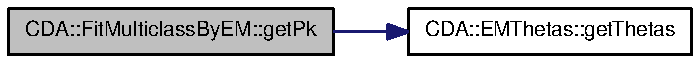
\includegraphics[width=176pt]{classCDA_1_1FitMulticlassByEM_a869530b76ee4b40d38d3fb80ea0932aa_cgraph}
\end{center}
\end{figure}




Hier ist ein Graph der zeigt, wo diese Funktion aufgerufen wird:\nopagebreak
\begin{figure}[H]
\begin{center}
\leavevmode
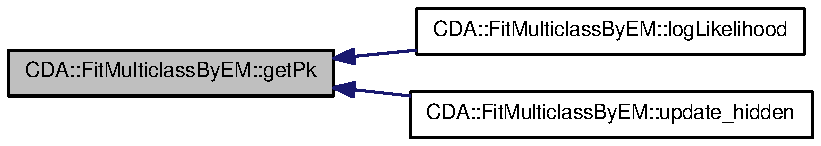
\includegraphics[width=215pt]{classCDA_1_1FitMulticlassByEM_a869530b76ee4b40d38d3fb80ea0932aa_icgraph}
\end{center}
\end{figure}


\hypertarget{classCDA_1_1FitMulticlassByEM_aceb43b0a386c8f8e112562cc3288b23d}{
\index{CDA::FitMulticlassByEM@{CDA::FitMulticlassByEM}!initClassif@{initClassif}}
\index{initClassif@{initClassif}!CDA::FitMulticlassByEM@{CDA::FitMulticlassByEM}}
\subsubsection[{initClassif}]{\setlength{\rightskip}{0pt plus 5cm}template$<$class data\_\-T , class theta\_\-T $>$ void FitMulticlassByEM::initClassif ()\hspace{0.3cm}{\ttfamily  \mbox{[}inline\mbox{]}}}}
\label{classCDA_1_1FitMulticlassByEM_aceb43b0a386c8f8e112562cc3288b23d}


Initialize class membership beliefs. 

\hypertarget{GaussianMixtureModel1D_8h_09_09_NOTE}{}\subsection{NOTE}\label{GaussianMixtureModel1D_8h_09_09_NOTE}
setData of derived classes must call this =$>$ done, defined setData here. can one be \char`\"{}using\char`\"{} a template fn? 

Hier ist ein Graph der zeigt, was diese Funktion aufruft:\nopagebreak
\begin{figure}[H]
\begin{center}
\leavevmode
\includegraphics[width=243pt]{classCDA_1_1FitMulticlassByEM_aceb43b0a386c8f8e112562cc3288b23d_cgraph}
\end{center}
\end{figure}




Hier ist ein Graph der zeigt, wo diese Funktion aufgerufen wird:\nopagebreak
\begin{figure}[H]
\begin{center}
\leavevmode
\includegraphics[width=285pt]{classCDA_1_1FitMulticlassByEM_aceb43b0a386c8f8e112562cc3288b23d_icgraph}
\end{center}
\end{figure}


\hypertarget{classCDA_1_1FitMulticlassByEM_abaea206aef382360246cf2a64dadc74c}{
\index{CDA::FitMulticlassByEM@{CDA::FitMulticlassByEM}!logLikelihood@{logLikelihood}}
\index{logLikelihood@{logLikelihood}!CDA::FitMulticlassByEM@{CDA::FitMulticlassByEM}}
\subsubsection[{logLikelihood}]{\setlength{\rightskip}{0pt plus 5cm}template$<$class data\_\-T , class theta\_\-T $>$ double FitMulticlassByEM::logLikelihood () const\hspace{0.3cm}{\ttfamily  \mbox{[}inline, virtual\mbox{]}}}}
\label{classCDA_1_1FitMulticlassByEM_abaea206aef382360246cf2a64dadc74c}


Implemented here. 

\begin{DoxyReturn}{Rückgabe}
If you really wanna know the logLikelihood value at current iteration. 
\end{DoxyReturn}


Implementiert \hyperlink{classCDA_1_1EM_affb4273a70cd7562cc5d517412c4fcdb}{CDA::EM$<$ data\_\-T, theta\_\-T $>$}.



Hier ist ein Graph der zeigt, was diese Funktion aufruft:\nopagebreak
\begin{figure}[H]
\begin{center}
\leavevmode
\includegraphics[width=293pt]{classCDA_1_1FitMulticlassByEM_abaea206aef382360246cf2a64dadc74c_cgraph}
\end{center}
\end{figure}


\hypertarget{classCDA_1_1FitMulticlassByEM_a7c40c5528a4b8b32e2455056f60d76de}{
\index{CDA::FitMulticlassByEM@{CDA::FitMulticlassByEM}!update\_\-hidden@{update\_\-hidden}}
\index{update\_\-hidden@{update\_\-hidden}!CDA::FitMulticlassByEM@{CDA::FitMulticlassByEM}}
\subsubsection[{update\_\-hidden}]{\setlength{\rightskip}{0pt plus 5cm}template$<$class data\_\-T , class theta\_\-T $>$ void FitMulticlassByEM::update\_\-hidden ()\hspace{0.3cm}{\ttfamily  \mbox{[}inline, protected, virtual\mbox{]}}}}
\label{classCDA_1_1FitMulticlassByEM_a7c40c5528a4b8b32e2455056f60d76de}


{\bfseries E-\/step}: update hidden attributes, i.e. classification 

\hypertarget{GaussianMixtureModel1D_8h_09_09_NOTE}{}\subsection{NOTE}\label{GaussianMixtureModel1D_8h_09_09_NOTE}
It is common to all multiclass (mixture model) problem formulations, thus not redefined in subclasses. 

Implementiert \hyperlink{classCDA_1_1EM_a587d80945cad21df1233dc22cb95671d}{CDA::EM$<$ data\_\-T, theta\_\-T $>$}.



Hier ist ein Graph der zeigt, was diese Funktion aufruft:\nopagebreak
\begin{figure}[H]
\begin{center}
\leavevmode
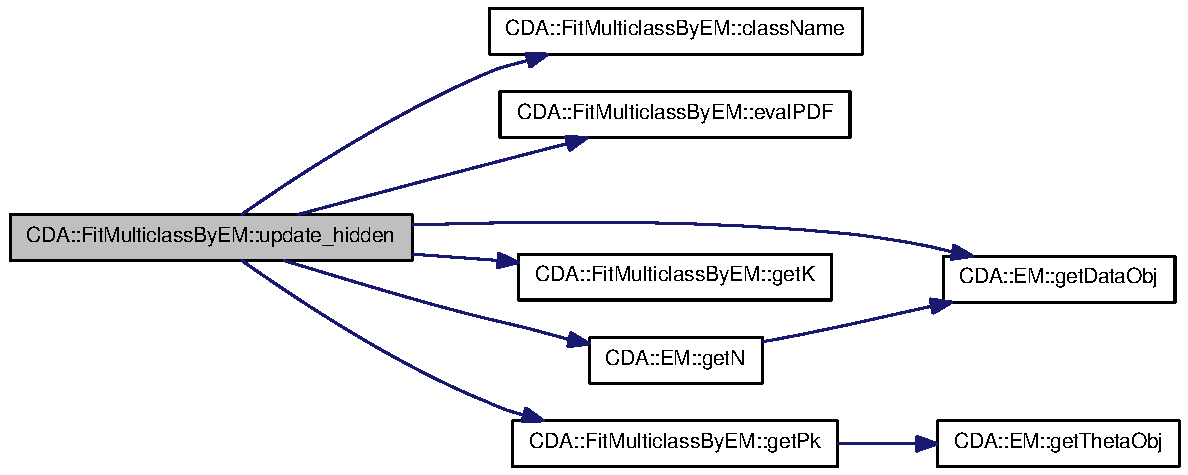
\includegraphics[width=303pt]{classCDA_1_1FitMulticlassByEM_a7c40c5528a4b8b32e2455056f60d76de_cgraph}
\end{center}
\end{figure}




Die Dokumentation für diese Klasse wurde erzeugt aufgrund der Dateien:\begin{DoxyCompactItemize}
\item 
include/expmax/\hyperlink{FitMulticlassByEM_8h_09_09}{FitMulticlassByEM.h++}\item 
src/expmax/\hyperlink{FitMulticlassByEM_8c_09_09}{FitMulticlassByEM.c++}\end{DoxyCompactItemize}

\hypertarget{classCDA_1_1FitMultivariateMulticlassByEM}{
\section{CDA::FitMultivariateMulticlassByEM$<$ theta\_\-T $>$ Template-\/Klassenreferenz}
\label{classCDA_1_1FitMultivariateMulticlassByEM}\index{CDA::FitMultivariateMulticlassByEM@{CDA::FitMultivariateMulticlassByEM}}
}


Note that the \hyperlink{classCDA_1_1EMData}{EMData} type is fixed: \hyperlink{classCDA_1_1VectorEMData}{VectorEMData}.  




{\ttfamily \#include $<$FitMultivariateMulticlassByEM.h++$>$}



Abgeleitet von \hyperlink{classCDA_1_1FitMulticlassByEM}{FitMulticlassByEM$<$ VectorEMData, theta\_\-T $>$}.



Basisklasse für \hyperlink{classCDA_1_1EMGenericMixtureModelCore}{CDA::EMGenericMixtureModelCore$<$ theta\_\-T $>$}.



Zusammengehörigkeiten von CDA::FitMultivariateMulticlassByEM$<$ theta\_\-T $>$:\nopagebreak
\begin{figure}[H]
\begin{center}
\leavevmode
\includegraphics[width=400pt]{classCDA_1_1FitMultivariateMulticlassByEM__coll__graph}
\end{center}
\end{figure}
\subsection*{Öffentliche Typen}
\begin{DoxyCompactItemize}
\item 
\hypertarget{classCDA_1_1FitMultivariateMulticlassByEM_a7831e85cafbf2f27c8944c9db1e4c4bf}{
typedef \hyperlink{classCDA_1_1VectorEMData}{VectorEMData} \hyperlink{classCDA_1_1FitMultivariateMulticlassByEM_a7831e85cafbf2f27c8944c9db1e4c4bf}{data\_\-t}}
\label{classCDA_1_1FitMultivariateMulticlassByEM_a7831e85cafbf2f27c8944c9db1e4c4bf}

\begin{DoxyCompactList}\small\item\em Define the datapoint\_\-t. \item\end{DoxyCompactList}\item 
\hypertarget{classCDA_1_1FitMultivariateMulticlassByEM_a25d1211b30d3b411a0116b8efd66efdf}{
typedef \hyperlink{classCDA_1_1EMData_a010a85bcffac375b7b0d9dfbc0ed2626}{VectorEMData::value\_\-type} {\bfseries datapoint\_\-t}}
\label{classCDA_1_1FitMultivariateMulticlassByEM_a25d1211b30d3b411a0116b8efd66efdf}

\item 
\hypertarget{classCDA_1_1FitMultivariateMulticlassByEM_afc08a4f0e2d114eefa4ac5e5894e78aa}{
typedef theta\_\-T {\bfseries theta\_\-t}}
\label{classCDA_1_1FitMultivariateMulticlassByEM_afc08a4f0e2d114eefa4ac5e5894e78aa}

\end{DoxyCompactItemize}
\subsection*{Öffentliche Methoden}
\begin{DoxyCompactItemize}
\item 
\hyperlink{classCDA_1_1FitMultivariateMulticlassByEM_ab16e1e3d2592e52801d7ebe94fb8b8d3}{FitMultivariateMulticlassByEM} (const unsigned K\_\-, const \hyperlink{classCDA_1_1VectorEMData}{VectorEMData} \&data, const theta\_\-t \&theta)
\begin{DoxyCompactList}\small\item\em Constructor. \item\end{DoxyCompactList}\item 
\hypertarget{classCDA_1_1FitMultivariateMulticlassByEM_a61354d086a158b075beccd1a956eb1f8}{
unsigned {\bfseries getD} () const }
\label{classCDA_1_1FitMultivariateMulticlassByEM_a61354d086a158b075beccd1a956eb1f8}

\end{DoxyCompactItemize}


\subsection{Ausführliche Beschreibung}
\subsubsection*{template$<$class theta\_\-T$>$ class CDA::FitMultivariateMulticlassByEM$<$ theta\_\-T $>$}

Note that the \hyperlink{classCDA_1_1EMData}{EMData} type is fixed: \hyperlink{classCDA_1_1VectorEMData}{VectorEMData}. It's no longer a simple typedef. 

\subsection{Beschreibung der Konstruktoren und Destruktoren}
\hypertarget{classCDA_1_1FitMultivariateMulticlassByEM_ab16e1e3d2592e52801d7ebe94fb8b8d3}{
\index{CDA::FitMultivariateMulticlassByEM@{CDA::FitMultivariateMulticlassByEM}!FitMultivariateMulticlassByEM@{FitMultivariateMulticlassByEM}}
\index{FitMultivariateMulticlassByEM@{FitMultivariateMulticlassByEM}!CDA::FitMultivariateMulticlassByEM@{CDA::FitMultivariateMulticlassByEM}}
\subsubsection[{FitMultivariateMulticlassByEM}]{\setlength{\rightskip}{0pt plus 5cm}template$<$class theta\_\-T$>$ {\bf CDA::FitMultivariateMulticlassByEM}$<$ theta\_\-T $>$::{\bf FitMultivariateMulticlassByEM} (const unsigned {\em K\_\-}, \/  const {\bf VectorEMData} \& {\em data}, \/  const theta\_\-t \& {\em theta})\hspace{0.3cm}{\ttfamily  \mbox{[}inline\mbox{]}}}}
\label{classCDA_1_1FitMultivariateMulticlassByEM_ab16e1e3d2592e52801d7ebe94fb8b8d3}


Constructor. 


\begin{DoxyParams}{Parameter}
\item[\mbox{$\leftarrow$} {\em K\_\-}]this way round, because of default parameter in superclass \item[\mbox{$\leftarrow$} {\em data}]D is not explicitly passed to this class anymore since not necessary, already in data. \item[\mbox{$\leftarrow$} {\em theta}]\end{DoxyParams}


Die Dokumentation für diese Klasse wurde erzeugt aufgrund der Dateien:\begin{DoxyCompactItemize}
\item 
include/expmax/\hyperlink{FitMultivariateMulticlassByEM_8h_09_09}{FitMultivariateMulticlassByEM.h++}\item 
src/expmax/\hyperlink{FitMultivariateMulticlassByEM_8c_09_09}{FitMultivariateMulticlassByEM.c++}\end{DoxyCompactItemize}

\include{classCDA_1_1FitUnivariateMulticlassByEM}
\hypertarget{classCDA_1_1GaussianMixtureModel}{
\section{CDA::GaussianMixtureModel Klassenreferenz}
\label{classCDA_1_1GaussianMixtureModel}\index{CDA::GaussianMixtureModel@{CDA::GaussianMixtureModel}}
}


Abgeleitet von \hyperlink{classCDA_1_1GaussianMixtureModelNDCommon}{CDA::GaussianMixtureModelNDCommon}.



Zusammengehörigkeiten von CDA::GaussianMixtureModel:\nopagebreak
\begin{figure}[H]
\begin{center}
\leavevmode
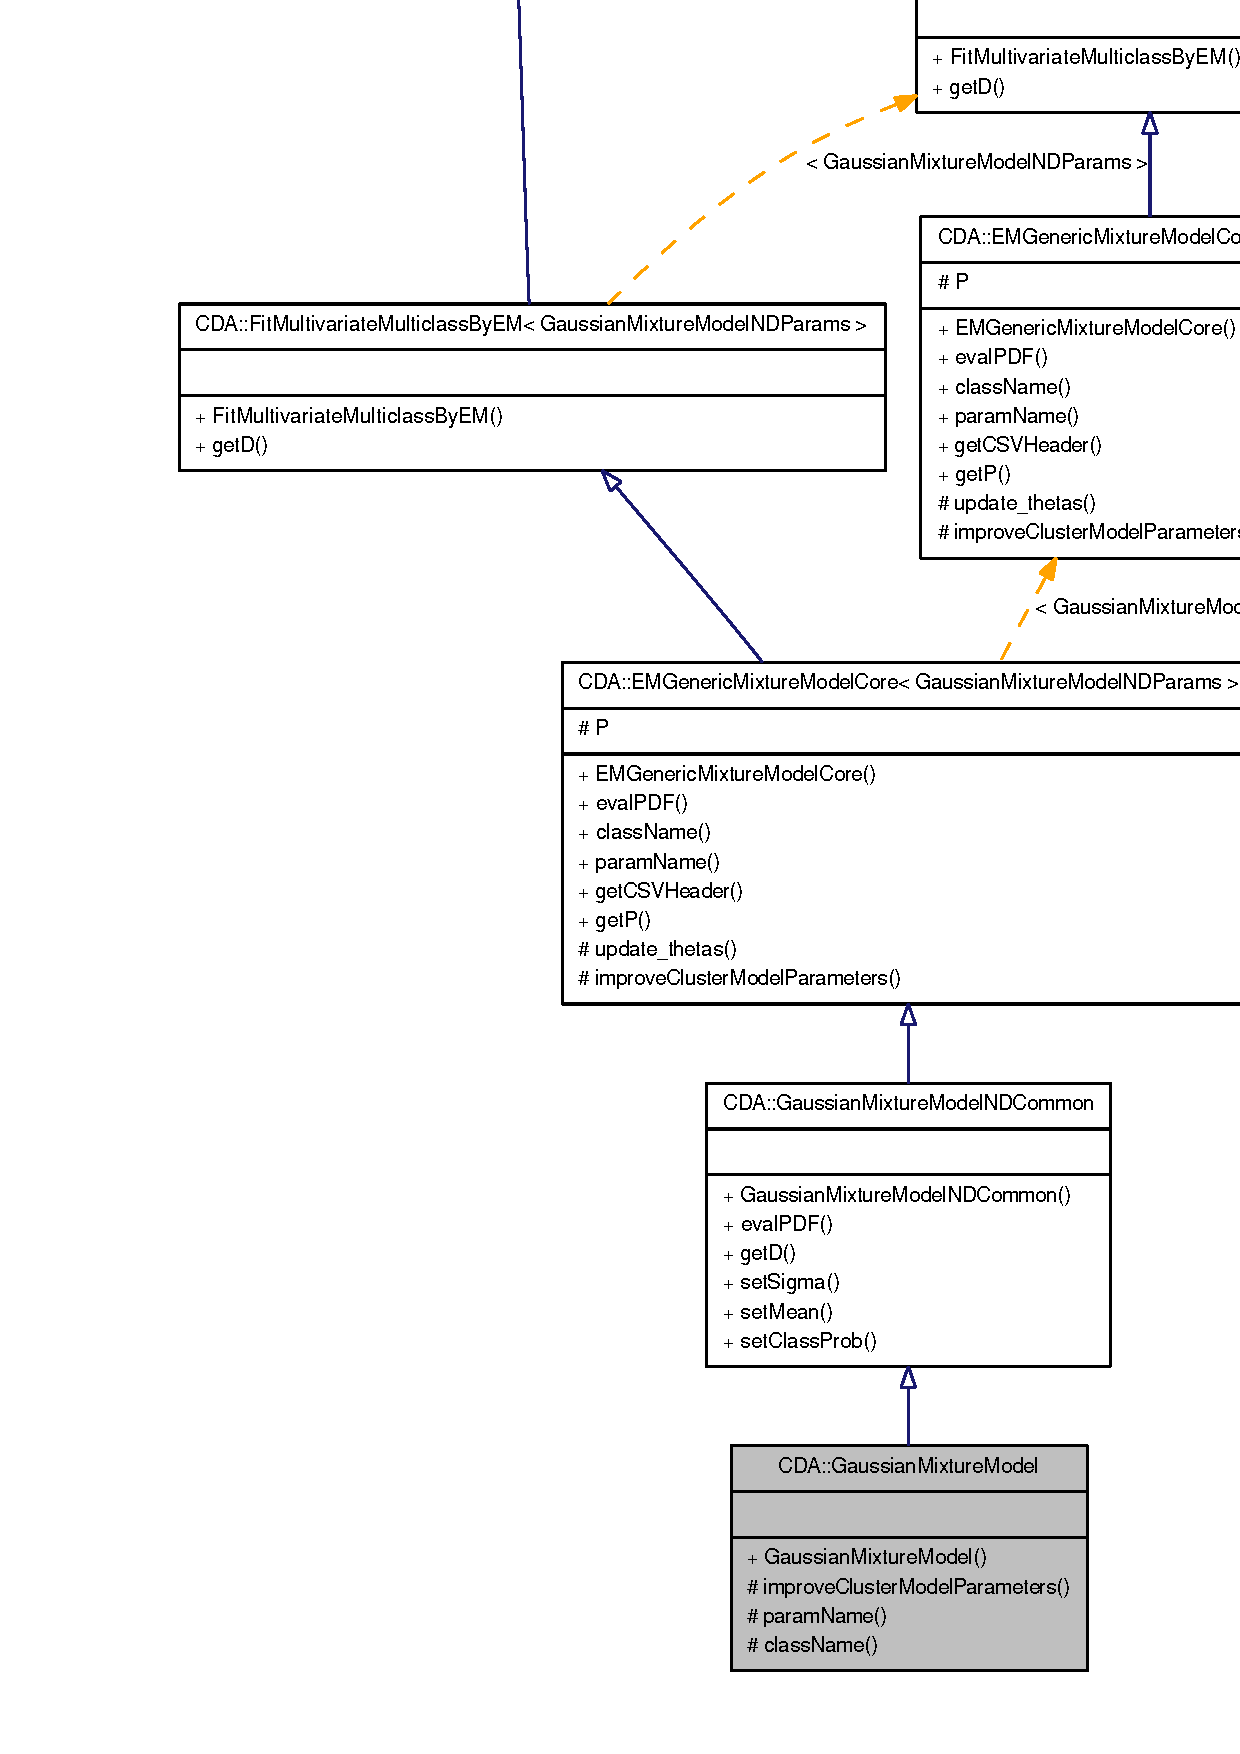
\includegraphics[width=400pt]{classCDA_1_1GaussianMixtureModel__coll__graph}
\end{center}
\end{figure}
\subsection*{Öffentliche Typen}
\begin{DoxyCompactItemize}
\item 
\hypertarget{classCDA_1_1GaussianMixtureModel_a1b5062d5be14d4e057f1cec50561057e}{
typedef GaussianMixtureModelNDCommon::datapoint\_\-t \hyperlink{classCDA_1_1GaussianMixtureModel_a1b5062d5be14d4e057f1cec50561057e}{datapoint\_\-t}}
\label{classCDA_1_1GaussianMixtureModel_a1b5062d5be14d4e057f1cec50561057e}

\begin{DoxyCompactList}\small\item\em Types. \item\end{DoxyCompactList}\item 
\hypertarget{classCDA_1_1GaussianMixtureModel_a97327ed10b2954b8cbb4a83c340b00da}{
typedef \hyperlink{classCDA_1_1GaussianMixtureModelNDCommon_a95dd5e5ca98ec39788d0de3b09d07a1a}{GaussianMixtureModelNDCommon::data\_\-t} \hyperlink{classCDA_1_1GaussianMixtureModel_a97327ed10b2954b8cbb4a83c340b00da}{data\_\-t}}
\label{classCDA_1_1GaussianMixtureModel_a97327ed10b2954b8cbb4a83c340b00da}

\begin{DoxyCompactList}\small\item\em Propagate the datapoint\_\-t. \item\end{DoxyCompactList}\item 
\hypertarget{classCDA_1_1GaussianMixtureModel_a5c0afb5b2f1626ec4b66f2f870f2cee9}{
typedef \hyperlink{classCDA_1_1GaussianMixtureModelNDParams}{GaussianMixtureModelNDCommon::theta\_\-t} {\bfseries theta\_\-t}}
\label{classCDA_1_1GaussianMixtureModel_a5c0afb5b2f1626ec4b66f2f870f2cee9}

\item 
\hypertarget{classCDA_1_1GaussianMixtureModel_a90bd1fd92303e6a52e8b269e7624b276}{
typedef GaussianMixtureModelNDCommon::theta\_\-t::sym\_\-mtx\_\-t {\bfseries sym\_\-mtx\_\-t}}
\label{classCDA_1_1GaussianMixtureModel_a90bd1fd92303e6a52e8b269e7624b276}

\end{DoxyCompactItemize}
\subsection*{Öffentliche Methoden}
\begin{DoxyCompactItemize}
\item 
\hyperlink{classCDA_1_1GaussianMixtureModel_a4ed542a3d6838511b11d22560f7dc9b4}{GaussianMixtureModel} (const unsigned K\_\-, const unsigned D\_\-, const \hyperlink{classCDA_1_1GaussianMixtureModel_a97327ed10b2954b8cbb4a83c340b00da}{data\_\-t} \&data, const \hyperlink{classCDA_1_1GaussianMixtureModelNDParams}{theta\_\-t} \&theta)
\begin{DoxyCompactList}\small\item\em Constructor. \item\end{DoxyCompactList}\end{DoxyCompactItemize}
\subsection*{Geschützte Methoden}
\begin{DoxyCompactItemize}
\item 
virtual void \hyperlink{classCDA_1_1GaussianMixtureModel_afe0080d43eb7169d66e57d074f1b7efc}{improveClusterModelParameters} ()
\begin{DoxyCompactList}\small\item\em The quasi-\/MLE step, part of {\bfseries E-\/step}. \item\end{DoxyCompactList}\item 
\hypertarget{classCDA_1_1GaussianMixtureModel_ace9d6f0ae0c45734c78be74b2c15d36b}{
virtual const std::string \hyperlink{classCDA_1_1GaussianMixtureModel_ace9d6f0ae0c45734c78be74b2c15d36b}{paramName} (const unsigned p) const }
\label{classCDA_1_1GaussianMixtureModel_ace9d6f0ae0c45734c78be74b2c15d36b}

\begin{DoxyCompactList}\small\item\em Construct names of parameters, e.g. for output calls same function from ...Common. \item\end{DoxyCompactList}\item 
virtual const std::string \hyperlink{classCDA_1_1GaussianMixtureModel_aec72323935694359e18e3363ceaa40e7}{className} () const 
\begin{DoxyCompactList}\small\item\em Class name for logging. \item\end{DoxyCompactList}\end{DoxyCompactItemize}


\subsection{Beschreibung der Konstruktoren und Destruktoren}
\hypertarget{classCDA_1_1GaussianMixtureModel_a4ed542a3d6838511b11d22560f7dc9b4}{
\index{CDA::GaussianMixtureModel@{CDA::GaussianMixtureModel}!GaussianMixtureModel@{GaussianMixtureModel}}
\index{GaussianMixtureModel@{GaussianMixtureModel}!CDA::GaussianMixtureModel@{CDA::GaussianMixtureModel}}
\subsubsection[{GaussianMixtureModel}]{\setlength{\rightskip}{0pt plus 5cm}CDA::GaussianMixtureModel::GaussianMixtureModel (const unsigned {\em K\_\-}, \/  const unsigned {\em D\_\-}, \/  const {\bf data\_\-t} \& {\em data}, \/  const {\bf theta\_\-t} \& {\em theta})\hspace{0.3cm}{\ttfamily  \mbox{[}inline\mbox{]}}}}
\label{classCDA_1_1GaussianMixtureModel_a4ed542a3d6838511b11d22560f7dc9b4}


Constructor. 


\begin{DoxyParams}{Parameter}
\item[\mbox{$\leftarrow$} {\em K\_\-}]this way round, because of default parameter in superclass \item[\mbox{$\leftarrow$} {\em D\_\-}]\item[\mbox{$\leftarrow$} {\em data}]\item[\mbox{$\leftarrow$} {\em theta}]\end{DoxyParams}


\subsection{Dokumentation der Elementfunktionen}
\hypertarget{classCDA_1_1GaussianMixtureModel_aec72323935694359e18e3363ceaa40e7}{
\index{CDA::GaussianMixtureModel@{CDA::GaussianMixtureModel}!className@{className}}
\index{className@{className}!CDA::GaussianMixtureModel@{CDA::GaussianMixtureModel}}
\subsubsection[{className}]{\setlength{\rightskip}{0pt plus 5cm}const std::string GaussianMixtureModel::className () const\hspace{0.3cm}{\ttfamily  \mbox{[}protected, virtual\mbox{]}}}}
\label{classCDA_1_1GaussianMixtureModel_aec72323935694359e18e3363ceaa40e7}


Class name for logging. 

\begin{DoxyReturn}{Rückgabe}

\end{DoxyReturn}


Erneute Implementation von \hyperlink{classCDA_1_1EMGenericMixtureModelCore_a6e444765b04615888d41c4ab6c82ae61}{CDA::EMGenericMixtureModelCore$<$ GaussianMixtureModelNDParams $>$}.



Hier ist ein Graph der zeigt, wo diese Funktion aufgerufen wird:\nopagebreak
\begin{figure}[H]
\begin{center}
\leavevmode
\includegraphics[width=282pt]{classCDA_1_1GaussianMixtureModel_aec72323935694359e18e3363ceaa40e7_icgraph}
\end{center}
\end{figure}


\hypertarget{classCDA_1_1GaussianMixtureModel_afe0080d43eb7169d66e57d074f1b7efc}{
\index{CDA::GaussianMixtureModel@{CDA::GaussianMixtureModel}!improveClusterModelParameters@{improveClusterModelParameters}}
\index{improveClusterModelParameters@{improveClusterModelParameters}!CDA::GaussianMixtureModel@{CDA::GaussianMixtureModel}}
\subsubsection[{improveClusterModelParameters}]{\setlength{\rightskip}{0pt plus 5cm}void GaussianMixtureModel::improveClusterModelParameters ()\hspace{0.3cm}{\ttfamily  \mbox{[}protected, virtual\mbox{]}}}}
\label{classCDA_1_1GaussianMixtureModel_afe0080d43eb7169d66e57d074f1b7efc}


The quasi-\/MLE step, part of {\bfseries E-\/step}. 

\hypertarget{classCDA_1_1GaussianMixtureModel_CALLED-FROM}{}\subsection{CALLED-\/FROM}\label{classCDA_1_1GaussianMixtureModel_CALLED-FROM}
It is called from update\_\-thetas, which is already defined in EMGenericMixtureModelCore.c++ 

Implementiert \hyperlink{classCDA_1_1EMGenericMixtureModelCore_aed2b50eb2bb8582204e186e3d5834c0a}{CDA::EMGenericMixtureModelCore$<$ GaussianMixtureModelNDParams $>$}.



Hier ist ein Graph der zeigt, was diese Funktion aufruft:\nopagebreak
\begin{figure}[H]
\begin{center}
\leavevmode
\includegraphics[width=420pt]{classCDA_1_1GaussianMixtureModel_afe0080d43eb7169d66e57d074f1b7efc_cgraph}
\end{center}
\end{figure}




Die Dokumentation für diese Klasse wurde erzeugt aufgrund der Dateien:\begin{DoxyCompactItemize}
\item 
include/expmax/\hyperlink{GaussianMixtureModel_8h_09_09}{GaussianMixtureModel.h++}\item 
src/expmax/\hyperlink{GaussianMixtureModel_8c_09_09}{GaussianMixtureModel.c++}\end{DoxyCompactItemize}

\hypertarget{classCDA_1_1GaussianMixtureModel1D}{
\section{CDA::GaussianMixtureModel1D Klassenreferenz}
\label{classCDA_1_1GaussianMixtureModel1D}\index{CDA::GaussianMixtureModel1D@{CDA::GaussianMixtureModel1D}}
}


{\ttfamily \#include $<$GaussianMixtureModel1D.h++$>$}



Abgeleitet von \hyperlink{classCDA_1_1FitMulticlassByEM}{CDA::FitMulticlassByEM$<$ double $>$}.



Zusammengehörigkeiten von CDA::GaussianMixtureModel1D:\nopagebreak
\begin{figure}[H]
\begin{center}
\leavevmode
\includegraphics[height=400pt]{classCDA_1_1GaussianMixtureModel1D__coll__graph}
\end{center}
\end{figure}
\subsection*{Öffentliche Typen}
\begin{DoxyCompactItemize}
\item 
\hypertarget{classCDA_1_1GaussianMixtureModel1D_a72f70fc9a6a659f61bcaf74597d82aa7}{
typedef double \hyperlink{classCDA_1_1GaussianMixtureModel1D_a72f70fc9a6a659f61bcaf74597d82aa7}{datapoint\_\-t}}
\label{classCDA_1_1GaussianMixtureModel1D_a72f70fc9a6a659f61bcaf74597d82aa7}

\begin{DoxyCompactList}\small\item\em Propagate the datapoint\_\-t. Why can't I give it the same name? Annoying. \item\end{DoxyCompactList}\end{DoxyCompactItemize}
\subsection*{Öffentliche Methoden}
\begin{DoxyCompactItemize}
\item 
double \hyperlink{classCDA_1_1GaussianMixtureModel1D_a0ee83653e92c833951631f300cfe338d}{evalPDF} (const unsigned k, const \hyperlink{classCDA_1_1GaussianMixtureModel1D_a72f70fc9a6a659f61bcaf74597d82aa7}{datapoint\_\-t} \&x) const 
\begin{DoxyCompactList}\small\item\em Evaluate the cluster model PDF with class parameters $k$ at $\vec{x}$. \item\end{DoxyCompactList}\item 
\hypertarget{classCDA_1_1GaussianMixtureModel1D_a31a8e94938ebe3e88f66bfbd5a90017f}{
\hyperlink{classCDA_1_1GaussianMixtureModel1D_a31a8e94938ebe3e88f66bfbd5a90017f}{GaussianMixtureModel1D} (const unsigned K\_\-)}
\label{classCDA_1_1GaussianMixtureModel1D_a31a8e94938ebe3e88f66bfbd5a90017f}

\begin{DoxyCompactList}\small\item\em Call superclass constructor to fill data fields. \item\end{DoxyCompactList}\item 
double \hyperlink{classCDA_1_1GaussianMixtureModel1D_abd992452517cd8f0efc8f5408f898e33}{getMean} (const unsigned k) const 
\begin{DoxyCompactList}\small\item\em Estimated parameter getter. Get current estimated mean vector of class k. \item\end{DoxyCompactList}\item 
double \hyperlink{classCDA_1_1GaussianMixtureModel1D_aa943f4410a27db1d9530b7c63e45b90b}{getSigma} (const unsigned k) const 
\begin{DoxyCompactList}\small\item\em Estimated parameter getter Get current estimated sigma of class k. \item\end{DoxyCompactList}\item 
{\footnotesize template$<$class II $>$ }\\void \hyperlink{classCDA_1_1GaussianMixtureModel1D_ada5a646f31d12697bc0fc66934a54dab}{setData} (std::pair$<$ II, II $>$ data\_\-)
\begin{DoxyCompactList}\small\item\em Initialize known samples, i.e. your data points. \item\end{DoxyCompactList}\item 
double \hyperlink{classCDA_1_1GaussianMixtureModel1D_af375c24f37a361437719bfe42b03fd4a}{findDecisionLimit} (const int k1, const int k2) const 
\begin{DoxyCompactList}\small\item\em Find explicit class boundary. \item\end{DoxyCompactList}\item 
\hypertarget{classCDA_1_1GaussianMixtureModel1D_a08a734c5b74bccda43429df49db58edf}{
const std::string \hyperlink{classCDA_1_1GaussianMixtureModel1D_a08a734c5b74bccda43429df49db58edf}{className} () const }
\label{classCDA_1_1GaussianMixtureModel1D_a08a734c5b74bccda43429df49db58edf}

\begin{DoxyCompactList}\small\item\em Class name for logging ... \item\end{DoxyCompactList}\item 
\hypertarget{classCDA_1_1GaussianMixtureModel1D_adfb929641e967030e9b63c6e53ea64c0}{
const std::string \hyperlink{classCDA_1_1GaussianMixtureModel1D_adfb929641e967030e9b63c6e53ea64c0}{getCSVHeader} () const }
\label{classCDA_1_1GaussianMixtureModel1D_adfb929641e967030e9b63c6e53ea64c0}

\begin{DoxyCompactList}\small\item\em Each class gets its own line, that's the easiest way. \item\end{DoxyCompactList}\end{DoxyCompactItemize}
\subsection*{Geschützte Methoden}
\begin{DoxyCompactItemize}
\item 
\hypertarget{classCDA_1_1GaussianMixtureModel1D_ac8215fdb213641c0cf49eeb2f6d4c045}{
void \hyperlink{classCDA_1_1GaussianMixtureModel1D_ac8215fdb213641c0cf49eeb2f6d4c045}{update\_\-thetas} ()}
\label{classCDA_1_1GaussianMixtureModel1D_ac8215fdb213641c0cf49eeb2f6d4c045}

\begin{DoxyCompactList}\small\item\em {\bfseries E-\/step}: update hidden attributes, i.e. class membership probabilities \item\end{DoxyCompactList}\end{DoxyCompactItemize}


\subsection{Ausführliche Beschreibung}
A \hyperlink{classCDA_1_1GaussianMixtureModel}{GaussianMixtureModel} class, with \hyperlink{classCDA_1_1EM}{EM} fitting routine built in 

\subsection{Dokumentation der Elementfunktionen}
\hypertarget{classCDA_1_1GaussianMixtureModel1D_a0ee83653e92c833951631f300cfe338d}{
\index{CDA::GaussianMixtureModel1D@{CDA::GaussianMixtureModel1D}!evalPDF@{evalPDF}}
\index{evalPDF@{evalPDF}!CDA::GaussianMixtureModel1D@{CDA::GaussianMixtureModel1D}}
\subsubsection[{evalPDF}]{\setlength{\rightskip}{0pt plus 5cm}double CDA::GaussianMixtureModel1D::evalPDF (const unsigned {\em k}, \/  const {\bf datapoint\_\-t} \& {\em x}) const\hspace{0.3cm}{\ttfamily  \mbox{[}inline, virtual\mbox{]}}}}
\label{classCDA_1_1GaussianMixtureModel1D_a0ee83653e92c833951631f300cfe338d}


Evaluate the cluster model PDF with class parameters $k$ at $\vec{x}$. 


\begin{DoxyParams}{Parameter}
\item[\mbox{$\leftarrow$} {\em k}]class \item[\mbox{$\leftarrow$} {\em x}]feature vector\end{DoxyParams}
\begin{DoxyReturn}{Rückgabe}
probability $p(x,k\vert\theta)$ 
\end{DoxyReturn}


Implementiert \hyperlink{classCDA_1_1FitMulticlassByEM_a5853c1889b12e567d2d9ab6c395dfe0d}{CDA::FitMulticlassByEM$<$ T $>$}.

\hypertarget{classCDA_1_1GaussianMixtureModel1D_af375c24f37a361437719bfe42b03fd4a}{
\index{CDA::GaussianMixtureModel1D@{CDA::GaussianMixtureModel1D}!findDecisionLimit@{findDecisionLimit}}
\index{findDecisionLimit@{findDecisionLimit}!CDA::GaussianMixtureModel1D@{CDA::GaussianMixtureModel1D}}
\subsubsection[{findDecisionLimit}]{\setlength{\rightskip}{0pt plus 5cm}double CDA::GaussianMixtureModel1D::findDecisionLimit (const int {\em k1}, \/  const int {\em k2}) const\hspace{0.3cm}{\ttfamily  \mbox{[}inline\mbox{]}}}}
\label{classCDA_1_1GaussianMixtureModel1D_af375c24f37a361437719bfe42b03fd4a}


Find explicit class boundary. 


\begin{DoxyParams}{Parameter}
\item[\mbox{$\leftarrow$} {\em k1}]Class 1 \item[\mbox{$\leftarrow$} {\em k2}]Class 2\end{DoxyParams}
\begin{DoxyReturn}{Rückgabe}
x$>$value: in class 2 
\end{DoxyReturn}


Hier ist ein Graph der zeigt, was diese Funktion aufruft:\nopagebreak
\begin{figure}[H]
\begin{center}
\leavevmode
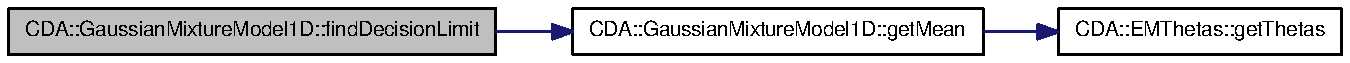
\includegraphics[width=342pt]{classCDA_1_1GaussianMixtureModel1D_af375c24f37a361437719bfe42b03fd4a_cgraph}
\end{center}
\end{figure}


\hypertarget{classCDA_1_1GaussianMixtureModel1D_abd992452517cd8f0efc8f5408f898e33}{
\index{CDA::GaussianMixtureModel1D@{CDA::GaussianMixtureModel1D}!getMean@{getMean}}
\index{getMean@{getMean}!CDA::GaussianMixtureModel1D@{CDA::GaussianMixtureModel1D}}
\subsubsection[{getMean}]{\setlength{\rightskip}{0pt plus 5cm}double GaussianMixtureModel1D::getMean (const unsigned {\em k}) const}}
\label{classCDA_1_1GaussianMixtureModel1D_abd992452517cd8f0efc8f5408f898e33}


Estimated parameter getter. Get current estimated mean vector of class k. 


\begin{DoxyParams}{Parameter}
\item[\mbox{$\leftarrow$} {\em k}]class no. \end{DoxyParams}


Hier ist ein Graph der zeigt, was diese Funktion aufruft:\nopagebreak
\begin{figure}[H]
\begin{center}
\leavevmode
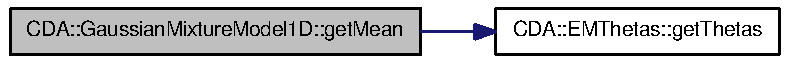
\includegraphics[width=207pt]{classCDA_1_1GaussianMixtureModel1D_abd992452517cd8f0efc8f5408f898e33_cgraph}
\end{center}
\end{figure}




Hier ist ein Graph der zeigt, wo diese Funktion aufgerufen wird:\nopagebreak
\begin{figure}[H]
\begin{center}
\leavevmode
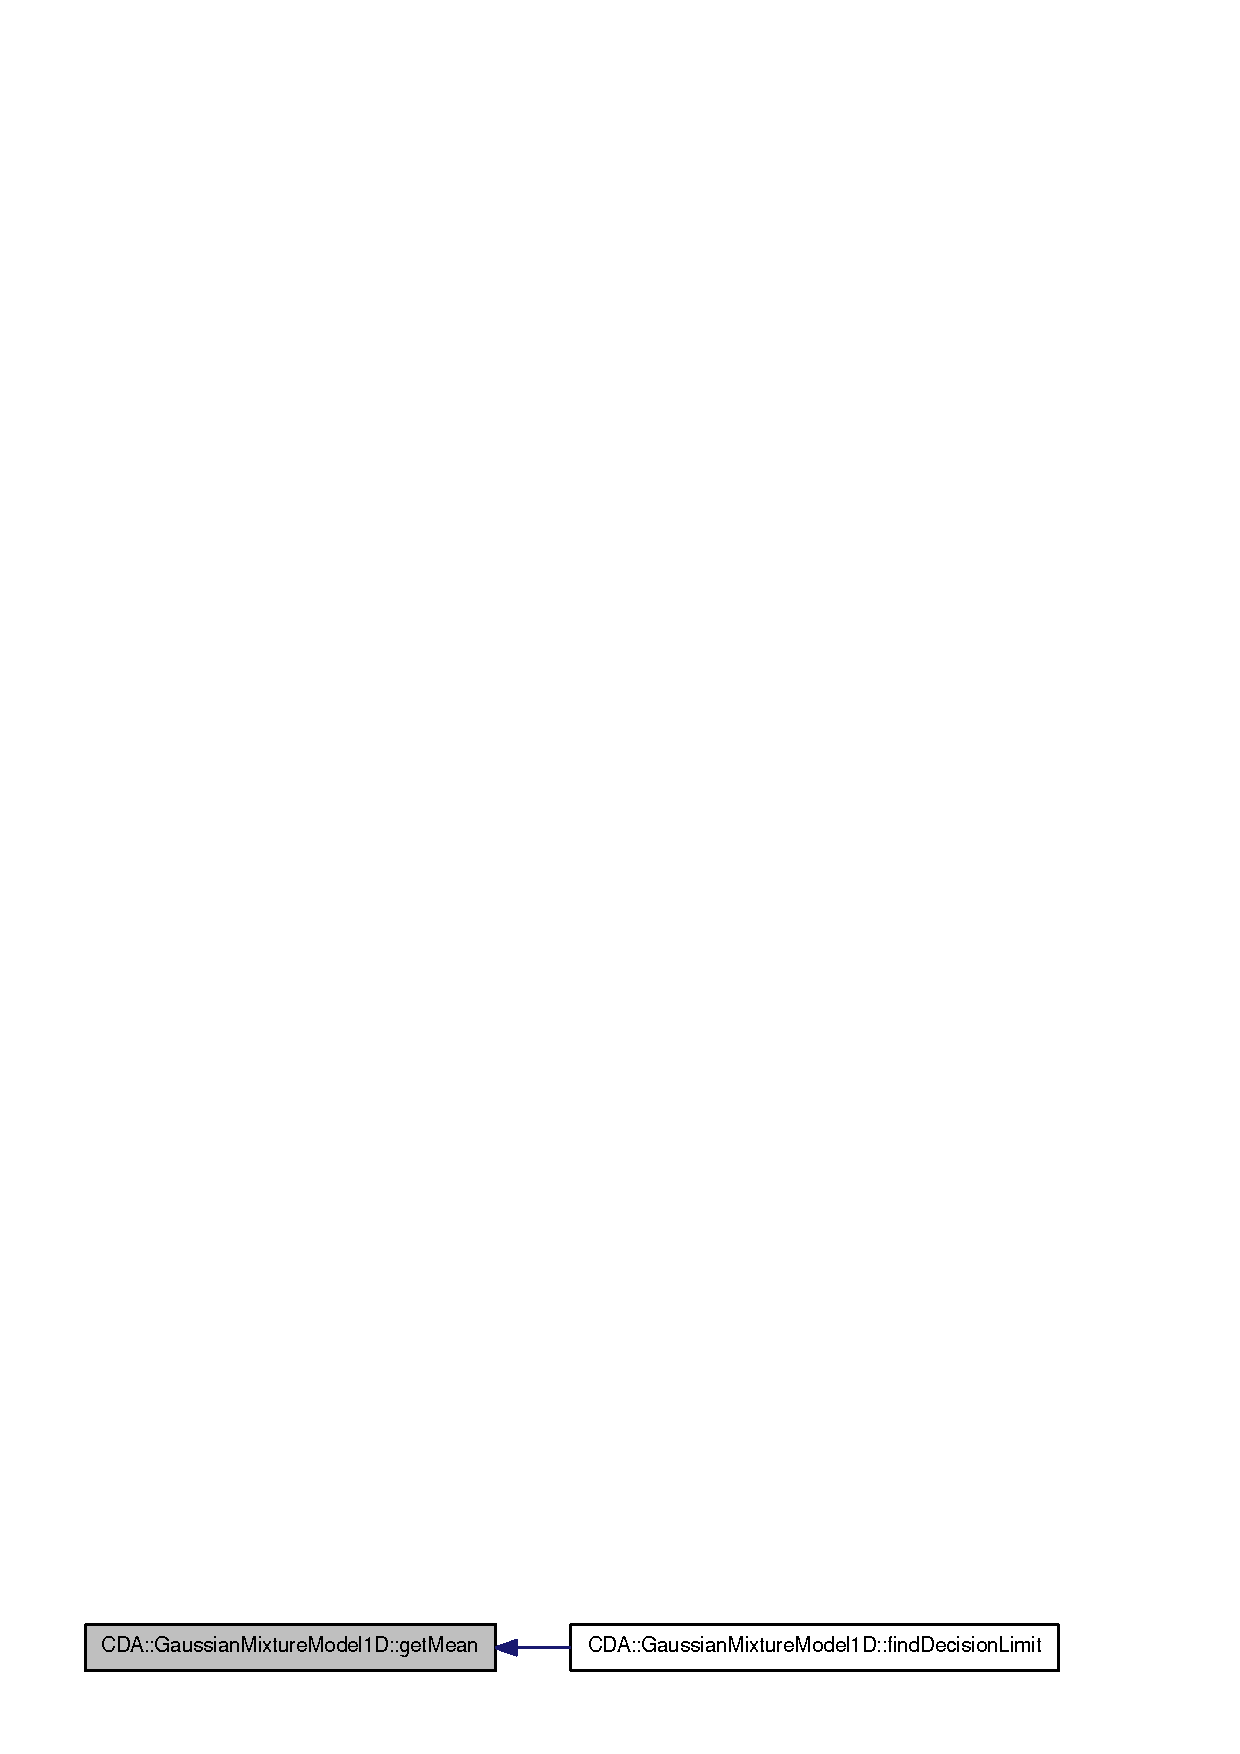
\includegraphics[width=256pt]{classCDA_1_1GaussianMixtureModel1D_abd992452517cd8f0efc8f5408f898e33_icgraph}
\end{center}
\end{figure}


\hypertarget{classCDA_1_1GaussianMixtureModel1D_aa943f4410a27db1d9530b7c63e45b90b}{
\index{CDA::GaussianMixtureModel1D@{CDA::GaussianMixtureModel1D}!getSigma@{getSigma}}
\index{getSigma@{getSigma}!CDA::GaussianMixtureModel1D@{CDA::GaussianMixtureModel1D}}
\subsubsection[{getSigma}]{\setlength{\rightskip}{0pt plus 5cm}double GaussianMixtureModel1D::getSigma (const unsigned {\em k}) const}}
\label{classCDA_1_1GaussianMixtureModel1D_aa943f4410a27db1d9530b7c63e45b90b}


Estimated parameter getter Get current estimated sigma of class k. 


\begin{DoxyParams}{Parameter}
\item[\mbox{$\leftarrow$} {\em k}]class no. \end{DoxyParams}


Hier ist ein Graph der zeigt, was diese Funktion aufruft:\nopagebreak
\begin{figure}[H]
\begin{center}
\leavevmode
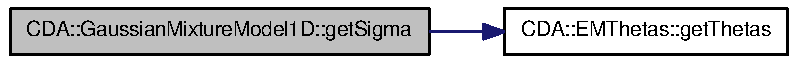
\includegraphics[width=209pt]{classCDA_1_1GaussianMixtureModel1D_aa943f4410a27db1d9530b7c63e45b90b_cgraph}
\end{center}
\end{figure}


\hypertarget{classCDA_1_1GaussianMixtureModel1D_ada5a646f31d12697bc0fc66934a54dab}{
\index{CDA::GaussianMixtureModel1D@{CDA::GaussianMixtureModel1D}!setData@{setData}}
\index{setData@{setData}!CDA::GaussianMixtureModel1D@{CDA::GaussianMixtureModel1D}}
\subsubsection[{setData}]{\setlength{\rightskip}{0pt plus 5cm}template$<$class II $>$ void CDA::GaussianMixtureModel1D::setData (std::pair$<$ II, II $>$ {\em data\_\-})\hspace{0.3cm}{\ttfamily  \mbox{[}inline\mbox{]}}}}
\label{classCDA_1_1GaussianMixtureModel1D_ada5a646f31d12697bc0fc66934a54dab}


Initialize known samples, i.e. your data points. 

Evaluate the PDF with parameters of class k


\begin{DoxyParams}{Parameter}
\item[\mbox{$\leftarrow$} {\em k}]class no. \item[\mbox{$\leftarrow$} {\em x}]\item[\mbox{$\leftarrow$} {\em data\_\-}]A pair of iterators. \end{DoxyParams}
\begin{Desc}
\item[\hyperlink{todo__todo000003}{Noch zu erledigen}]we should check II for compliance. \end{Desc}


Erneute Implementation von \hyperlink{classCDA_1_1FitMulticlassByEM_a7381428ebb707dbdd0553d6bc0e7113b}{CDA::FitMulticlassByEM$<$ T $>$}.



Die Dokumentation für diese Klasse wurde erzeugt aufgrund der Dateien:\begin{DoxyCompactItemize}
\item 
src/expmax/\hyperlink{GaussianMixtureModel1D_8h_09_09}{GaussianMixtureModel1D.h++}\item 
src/expmax/\hyperlink{ProbabilisticClustering_8c_09_09}{ProbabilisticClustering.c++}\end{DoxyCompactItemize}

\include{classGaussianMixtureModelNDClosedForm}
\include{classCDA_1_1GaussianMixtureModelNDCommon}
\include{classCDA_1_1GaussianMixtureModelNDParams}
\include{classCDA_1_1VectorEMData}
\hypertarget{structCDA_1_1VonMises}{
\section{CDA::VonMises Strukturreferenz}
\label{structCDA_1_1VonMises}\index{CDA::VonMises@{CDA::VonMises}}
}


{\ttfamily \#include $<$CircularStatistics.h++$>$}

\subsection*{Öffentliche Methoden}
\begin{DoxyCompactItemize}
\item 
double \hyperlink{structCDA_1_1VonMises_a85bd82b40dd422b2c044bb31bbaede58}{operator()} (const double mu, const double kappa, const double phi) const 
\item 
double \hyperlink{structCDA_1_1VonMises_a3ea11829bbcebe3dbfc174deda47cf9f}{deriv\_\-mu} (const double mu, const double kappa, const double phi) const 
\item 
double \hyperlink{structCDA_1_1VonMises_a392aea12f3aa6fc317342e92353783f9}{deriv\_\-kappa} (const double mu, const double kappa, const double phi) const 
\end{DoxyCompactItemize}


\subsection{Ausführliche Beschreibung}
Von Mises PDF and derivatives for circular statistics

(it approximates a wrapped Gaussian for small $Kappa$ and becomes a uniform distribution for large $Kappa$). 

\subsection{Dokumentation der Elementfunktionen}
\hypertarget{structCDA_1_1VonMises_a392aea12f3aa6fc317342e92353783f9}{
\index{CDA::VonMises@{CDA::VonMises}!deriv\_\-kappa@{deriv\_\-kappa}}
\index{deriv\_\-kappa@{deriv\_\-kappa}!CDA::VonMises@{CDA::VonMises}}
\subsubsection[{deriv\_\-kappa}]{\setlength{\rightskip}{0pt plus 5cm}double CDA::VonMises::deriv\_\-kappa (const double {\em mu}, \/  const double {\em kappa}, \/  const double {\em phi}) const\hspace{0.3cm}{\ttfamily  \mbox{[}inline\mbox{]}}}}
\label{structCDA_1_1VonMises_a392aea12f3aa6fc317342e92353783f9}
Get the value of $\frac{\partial M}{\partial \kappa}$

Important for parameter estimation \hypertarget{structCDA_1_1VonMises_a3ea11829bbcebe3dbfc174deda47cf9f}{
\index{CDA::VonMises@{CDA::VonMises}!deriv\_\-mu@{deriv\_\-mu}}
\index{deriv\_\-mu@{deriv\_\-mu}!CDA::VonMises@{CDA::VonMises}}
\subsubsection[{deriv\_\-mu}]{\setlength{\rightskip}{0pt plus 5cm}double CDA::VonMises::deriv\_\-mu (const double {\em mu}, \/  const double {\em kappa}, \/  const double {\em phi}) const\hspace{0.3cm}{\ttfamily  \mbox{[}inline\mbox{]}}}}
\label{structCDA_1_1VonMises_a3ea11829bbcebe3dbfc174deda47cf9f}
Get the value of $\frac{\partial M}{\partial \mu}$

Important for parameter estimation \hypertarget{structCDA_1_1VonMises_a85bd82b40dd422b2c044bb31bbaede58}{
\index{CDA::VonMises@{CDA::VonMises}!operator()@{operator()}}
\index{operator()@{operator()}!CDA::VonMises@{CDA::VonMises}}
\subsubsection[{operator()}]{\setlength{\rightskip}{0pt plus 5cm}double CDA::VonMises::operator() (const double {\em mu}, \/  const double {\em kappa}, \/  const double {\em phi}) const\hspace{0.3cm}{\ttfamily  \mbox{[}inline\mbox{]}}}}
\label{structCDA_1_1VonMises_a85bd82b40dd422b2c044bb31bbaede58}
Get the function value

\[ M(\mu, \kappa, x) = \frac{\exp{\kappa \cdot cos (x-\mu)}}{2\pi I_0 (\kappa)} \] 

Die Dokumentation für diese Struktur wurde erzeugt aufgrund der Datei:\begin{DoxyCompactItemize}
\item 
include/math/\hyperlink{CircularStatistics_8h_09_09}{CircularStatistics.h++}\end{DoxyCompactItemize}

\chapter{Datei-\/Dokumentation}
\hypertarget{common__definitions_8h_09_09}{
\section{include/common\_\-definitions.h++-\/Dateireferenz}
\label{common__definitions_8h_09_09}\index{include/common\_\-definitions.h++@{include/common\_\-definitions.h++}}
}
{\ttfamily \#include $<$boost/numeric/ublas/vector.hpp$>$}\par
{\ttfamily \#include $<$boost/numeric/ublas/io.hpp$>$}\par
Include-\/Abhängigkeitsdiagramm für common\_\-definitions.h++:\nopagebreak
\begin{figure}[H]
\begin{center}
\leavevmode
\includegraphics[width=173pt]{common__definitions_8h_09_09__incl}
\end{center}
\end{figure}
Dieser Graph zeigt, welche Datei direkt oder indirekt diese Datei enthält:\nopagebreak
\begin{figure}[H]
\begin{center}
\leavevmode
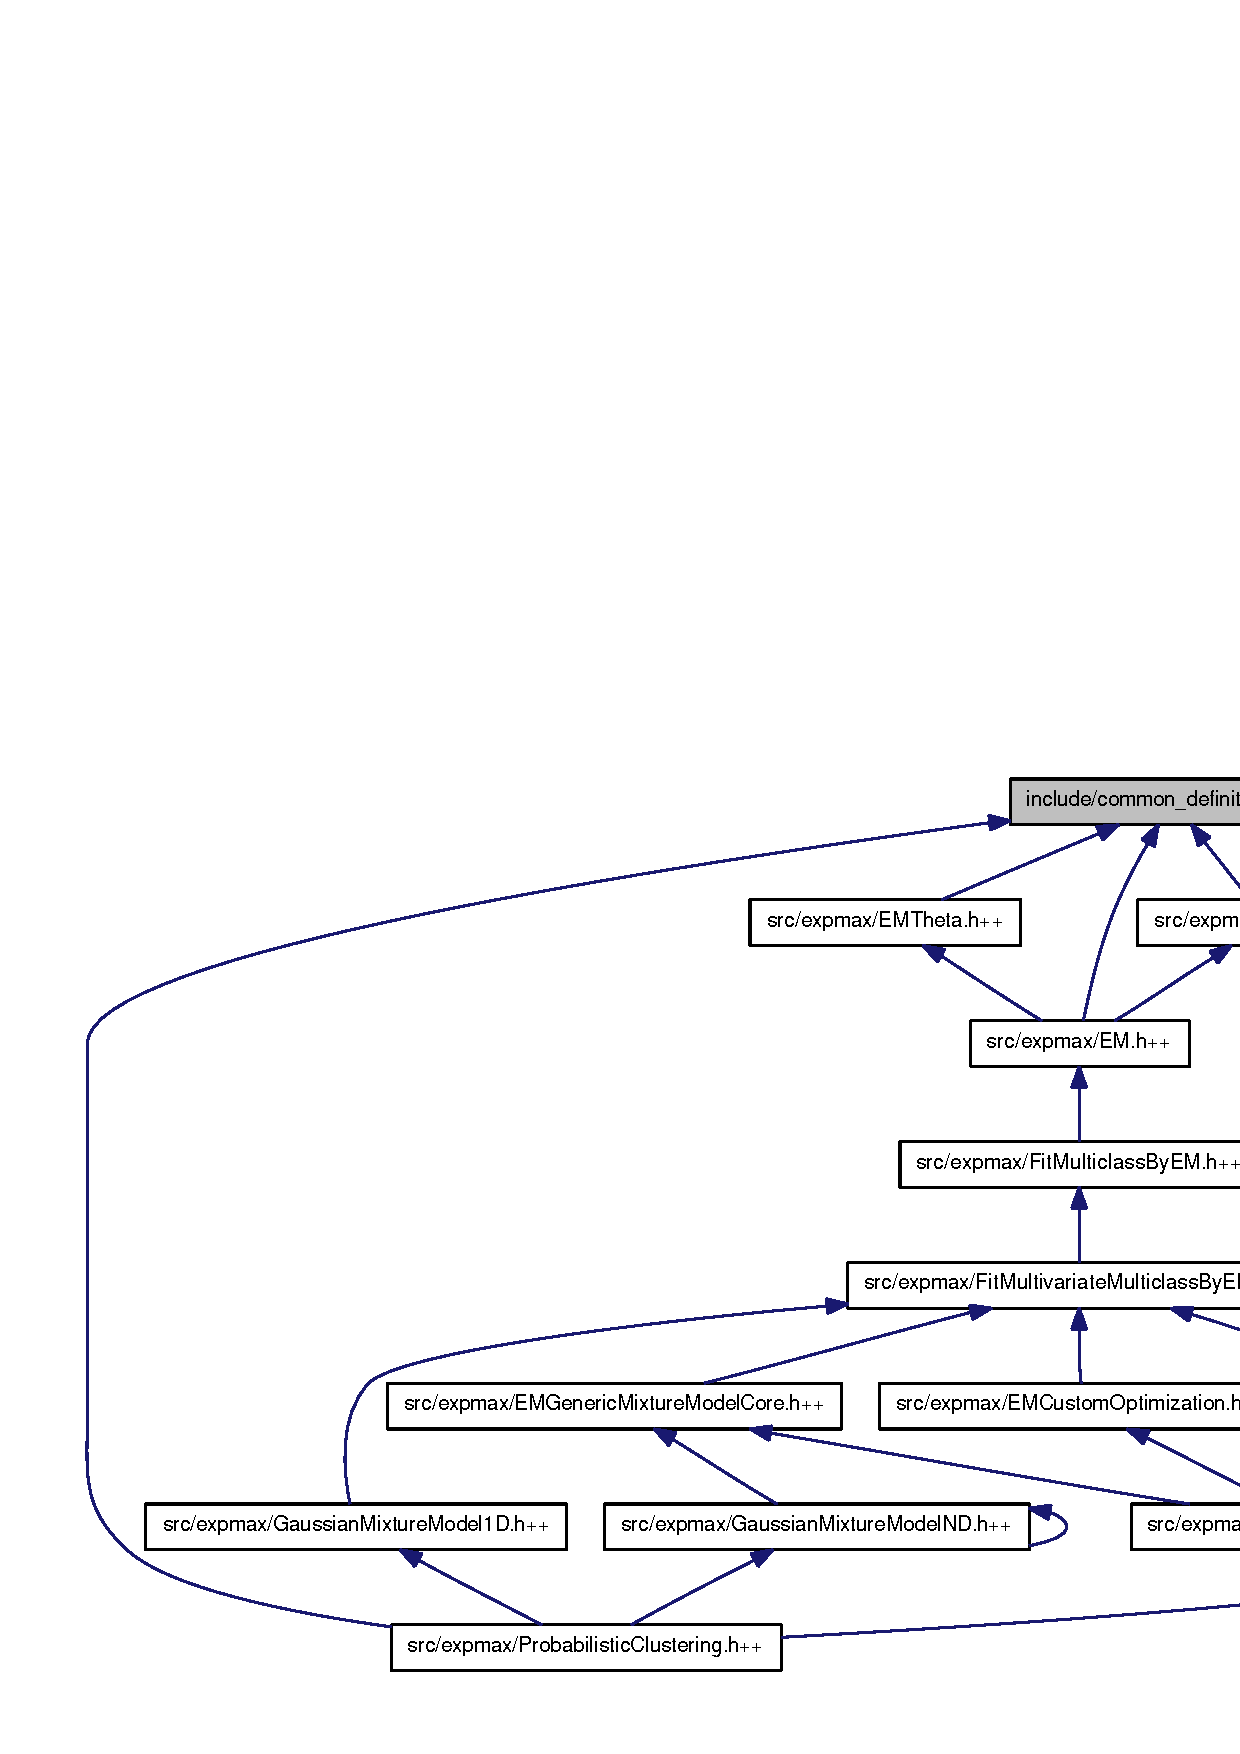
\includegraphics[width=420pt]{common__definitions_8h_09_09__dep__incl}
\end{center}
\end{figure}
\subsection*{Typdefinitionen}
\begin{DoxyCompactItemize}
\item 
\hypertarget{namespaceCDA_a6e1529c406401d049c61501e25d557e6}{
typedef boost::numeric::ublas::vector$<$ double $>$ \hyperlink{namespaceCDA_a6e1529c406401d049c61501e25d557e6}{CDA::fvector\_\-t}}
\label{namespaceCDA_a6e1529c406401d049c61501e25d557e6}

\begin{DoxyCompactList}\small\item\em Common declaration: Vector type. \item\end{DoxyCompactList}\end{DoxyCompactItemize}


\subsection{Ausführliche Beschreibung}
\begin{DoxyAuthor}{Autor}
Erik Flick $<$erik.flick \mbox{[}AETT\mbox{]} informatik.uni-\/hamburg.de$>$
\end{DoxyAuthor}
Created on: Jan 5, 2011 
\hypertarget{Data_8h_09_09}{
\section{include/data/Data.h++-\/Dateireferenz}
\label{Data_8h_09_09}\index{include/data/Data.h++@{include/data/Data.h++}}
}
{\ttfamily \#include $<$boost/foreach.hpp$>$}\par
{\ttfamily \#include $<$boost/numeric/ublas/storage.hpp$>$}\par
{\ttfamily \#include $<$boost/numeric/ublas/vector.hpp$>$}\par
{\ttfamily \#include $<$vector$>$}\par
{\ttfamily \#include $<$iostream$>$}\par
{\ttfamily \#include $<$algorithm$>$}\par
{\ttfamily \#include $<$boost/accumulators/accumulators.hpp$>$}\par
{\ttfamily \#include $<$boost/accumulators/statistics/min.hpp$>$}\par
{\ttfamily \#include $<$boost/accumulators/statistics/max.hpp$>$}\par
{\ttfamily \#include $<$boost/accumulators/statistics/stats.hpp$>$}\par
{\ttfamily \#include $<$boost/accumulators/statistics/mean.hpp$>$}\par
{\ttfamily \#include $<$boost/accumulators/statistics/moment.hpp$>$}\par
{\ttfamily \#include $<$boost/accumulators/statistics/variance.hpp$>$}\par
{\ttfamily \#include $<$boost/accumulators/statistics/covariance.hpp$>$}\par
{\ttfamily \#include $<$boost/iterator/filter\_\-iterator.hpp$>$}\par
{\ttfamily \#include $<$boost/iterator/transform\_\-iterator.hpp$>$}\par
{\ttfamily \#include $<$boost/function.hpp$>$}\par
{\ttfamily \#include $<$boost/lambda/lambda.hpp$>$}\par
{\ttfamily \#include $<$boost/lambda/bind.hpp$>$}\par
{\ttfamily \#include $<$boost/mem\_\-fn.hpp$>$}\par
{\ttfamily \#include $<$boost/bind.hpp$>$}\par
{\ttfamily \#include $<$boost/bind/arg.hpp$>$}\par
{\ttfamily \#include $<$boost/bind/placeholders.hpp$>$}\par
{\ttfamily \#include $<$boost/bind/mem\_\-fn.hpp$>$}\par
Include-\/Abhängigkeitsdiagramm für Data.h++:\nopagebreak
\begin{figure}[H]
\begin{center}
\leavevmode
\includegraphics[width=420pt]{Data_8h_09_09__incl}
\end{center}
\end{figure}
\subsection*{Klassen}
\begin{DoxyCompactItemize}
\item 
class \hyperlink{classCDA_1_1EnhancedDatasetView}{CDA::EnhancedDatasetView}
\item 
class \hyperlink{classCDA_1_1EnhancedDataset}{CDA::EnhancedDataset}
\begin{DoxyCompactList}\small\item\em aware of basic statistics for normalization etc. \item\end{DoxyCompactList}\end{DoxyCompactItemize}


\subsection{Ausführliche Beschreibung}
\begin{DoxyVersion}{Version}
0.02 
\end{DoxyVersion}
\begin{DoxyAuthor}{Autor}
Erik Flick $<$erik.flick \mbox{[}AETT\mbox{]} informatik.uni-\/hamburg.de$>$
\end{DoxyAuthor}
Created on: Dec 30, 2010\hypertarget{ProbabilisticClustering_8h_09_09_LICENSE}{}\subsection{LICENSE}\label{ProbabilisticClustering_8h_09_09_LICENSE}
LGPL v3.0

Sense the POWER!

Beginnings of a GNU R-\/like dataframe infrastructure. 
\hypertarget{EM_8h_09_09}{
\section{include/expmax/EM.h++-\/Dateireferenz}
\label{EM_8h_09_09}\index{include/expmax/EM.h++@{include/expmax/EM.h++}}
}
{\ttfamily \#include \char`\"{}EMData.h++\char`\"{}}\par
{\ttfamily \#include \char`\"{}common\_\-definitions.h++\char`\"{}}\par
{\ttfamily \#include $<$typeinfo$>$}\par
{\ttfamily \#include $<$boost/optional.hpp$>$}\par
{\ttfamily \#include $<$boost/mpl/equal.hpp$>$}\par
{\ttfamily \#include $<$boost/mpl/assert.hpp$>$}\par
Include-\/Abhängigkeitsdiagramm für EM.h++:\nopagebreak
\begin{figure}[H]
\begin{center}
\leavevmode
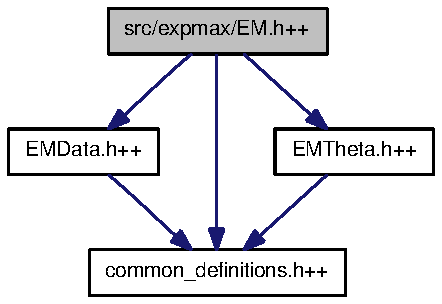
\includegraphics[width=345pt]{EM_8h_09_09__incl}
\end{center}
\end{figure}
Dieser Graph zeigt, welche Datei direkt oder indirekt diese Datei enthält:\nopagebreak
\begin{figure}[H]
\begin{center}
\leavevmode
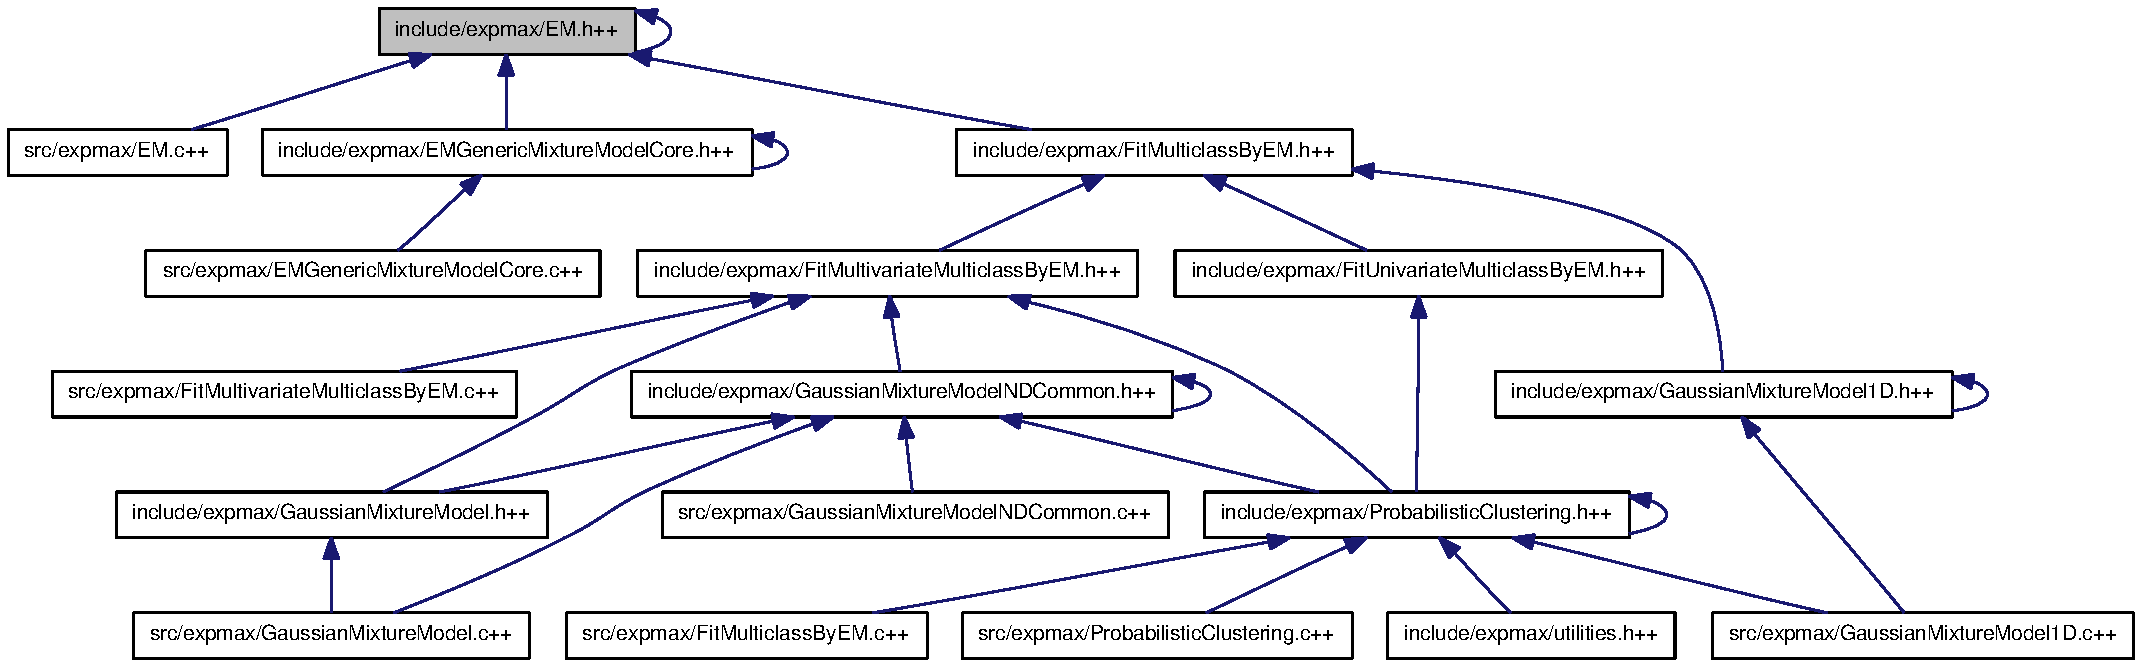
\includegraphics[width=420pt]{EM_8h_09_09__dep__incl}
\end{center}
\end{figure}
\subsection*{Klassen}
\begin{DoxyCompactItemize}
\item 
class \hyperlink{classCDA_1_1EM}{CDA::EM$<$ data\_\-T, theta\_\-T $>$}
\begin{DoxyCompactList}\small\item\em A generic \hyperlink{classCDA_1_1EM}{EM} model fitting class. \item\end{DoxyCompactList}\end{DoxyCompactItemize}


\subsection{Ausführliche Beschreibung}
\begin{DoxyVersion}{Version}
0.12 
\end{DoxyVersion}
\begin{DoxyAuthor}{Autor}
Erik Flick $<$erik.flick \mbox{[}AETT\mbox{]} informatik.uni-\/hamburg.de$>$
\end{DoxyAuthor}
Created on: Jan 5, 2011 
\hypertarget{EMData_8h_09_09}{
\section{src/expmax/EMData.h++-\/Dateireferenz}
\label{EMData_8h_09_09}\index{src/expmax/EMData.h++@{src/expmax/EMData.h++}}
}
{\ttfamily \#include \char`\"{}common\_\-definitions.h++\char`\"{}}\par
Include-\/Abhängigkeitsdiagramm für EMData.h++:\nopagebreak
\begin{figure}[H]
\begin{center}
\leavevmode
\includegraphics[width=85pt]{EMData_8h_09_09__incl}
\end{center}
\end{figure}
Dieser Graph zeigt, welche Datei direkt oder indirekt diese Datei enthält:\nopagebreak
\begin{figure}[H]
\begin{center}
\leavevmode
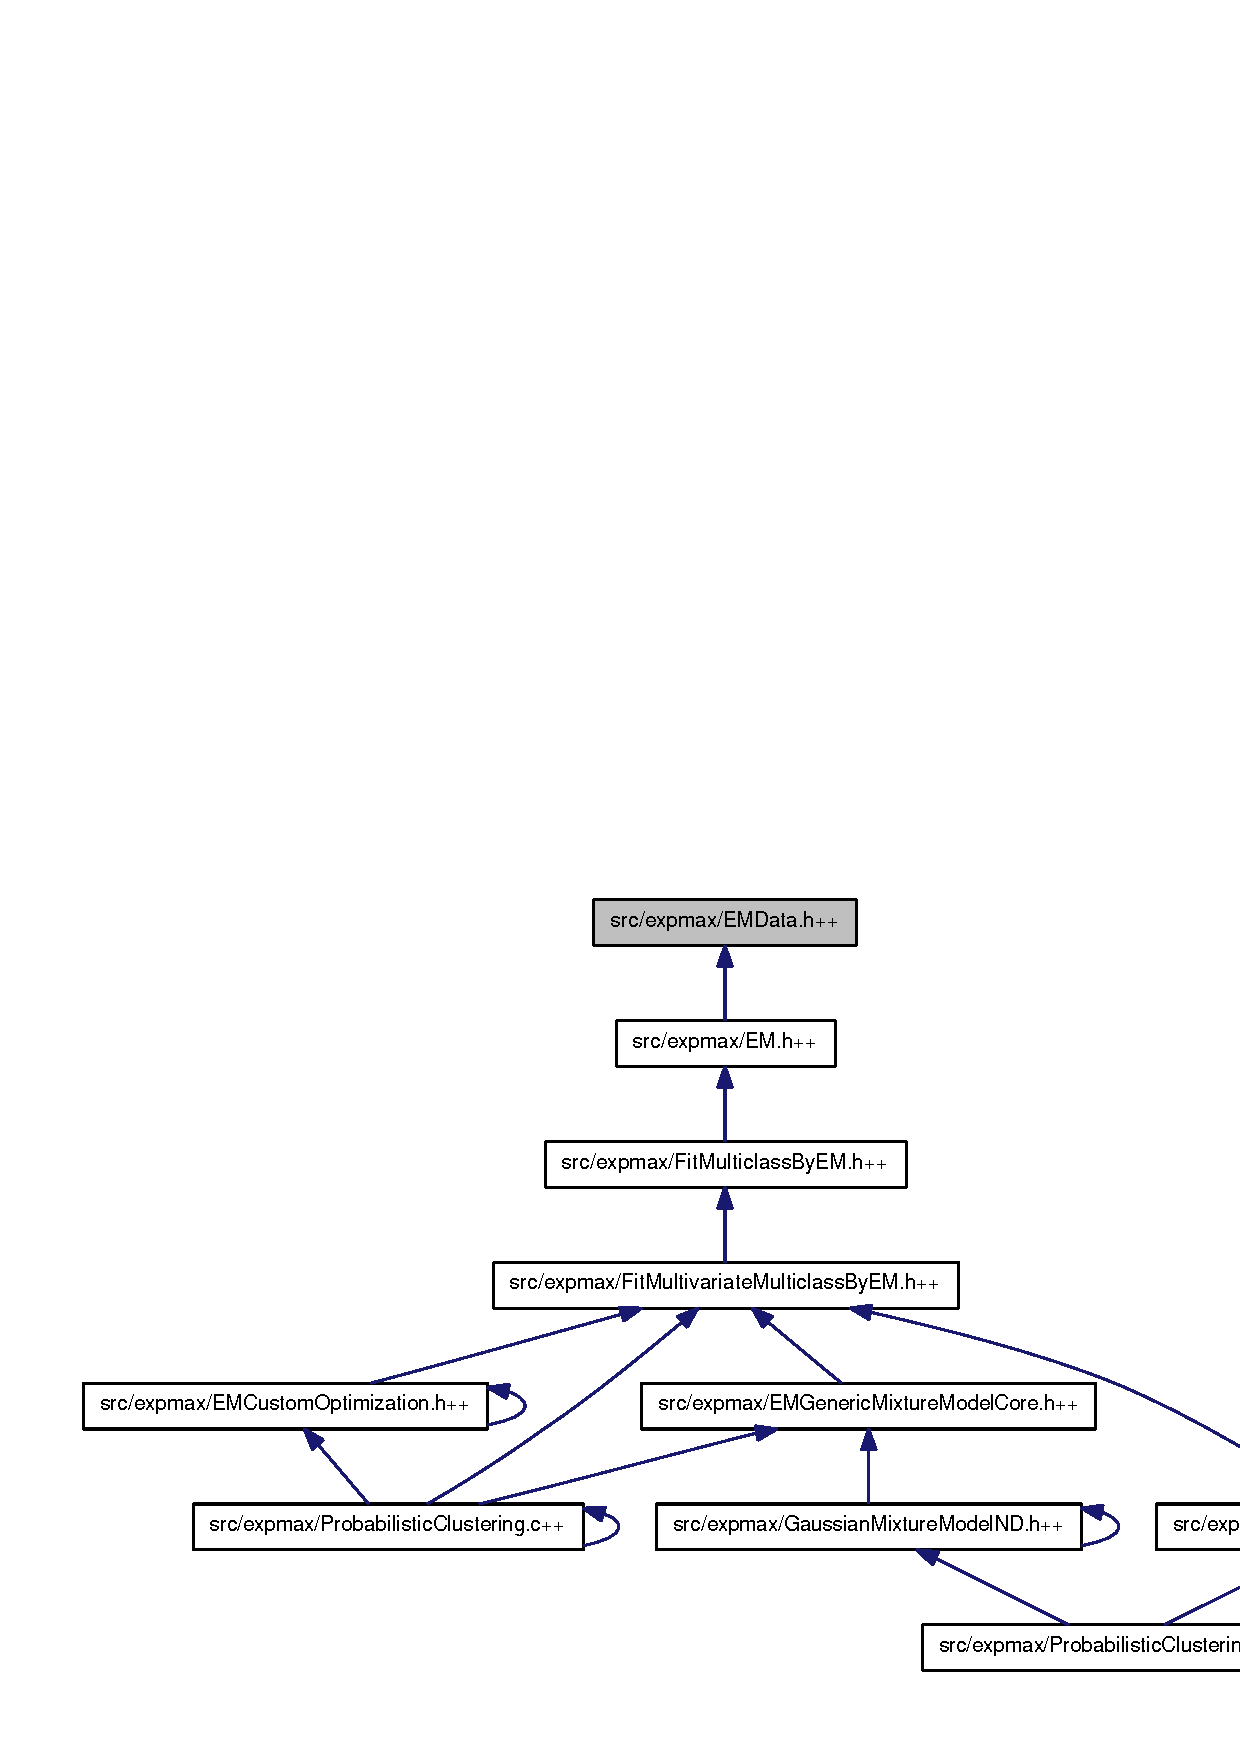
\includegraphics[width=380pt]{EMData_8h_09_09__dep__incl}
\end{center}
\end{figure}
\subsection*{Klassen}
\begin{DoxyCompactItemize}
\item 
class \hyperlink{classCDA_1_1EMData}{CDA::EMData$<$ T $>$}
\begin{DoxyCompactList}\small\item\em Any concrete \hyperlink{classCDA_1_1EM}{EM} subclass \char`\"{}has\_\-a\char`\"{} \hyperlink{classCDA_1_1EMData}{EMData} of the appropriate type (i.e. mono-\/ or multivariate). \item\end{DoxyCompactList}\end{DoxyCompactItemize}


\subsection{Ausführliche Beschreibung}
\begin{DoxyAuthor}{Autor}
Erik Flick $<$erik.flick \mbox{[}AETT\mbox{]} informatik.uni-\/hamburg.de$>$
\end{DoxyAuthor}
Created on: Jan 5, 2011 
\hypertarget{EMGenericMixtureModelCore_8h_09_09}{
\section{src/expmax/EMGenericMixtureModelCore.h++-\/Dateireferenz}
\label{EMGenericMixtureModelCore_8h_09_09}\index{src/expmax/EMGenericMixtureModelCore.h++@{src/expmax/EMGenericMixtureModelCore.h++}}
}
{\ttfamily \#include \char`\"{}FitMultivariateMulticlassByEM.h++\char`\"{}}\par
Include-\/Abhängigkeitsdiagramm für EMGenericMixtureModelCore.h++:\nopagebreak
\begin{figure}[H]
\begin{center}
\leavevmode
\includegraphics[width=131pt]{EMGenericMixtureModelCore_8h_09_09__incl}
\end{center}
\end{figure}
Dieser Graph zeigt, welche Datei direkt oder indirekt diese Datei enthält:\nopagebreak
\begin{figure}[H]
\begin{center}
\leavevmode
\includegraphics[width=244pt]{EMGenericMixtureModelCore_8h_09_09__dep__incl}
\end{center}
\end{figure}
\subsection*{Klassen}
\begin{DoxyCompactItemize}
\item 
class \hyperlink{classCDA_1_1EMGenericMixtureModelCore}{CDA::EMGenericMixtureModelCore}
\begin{DoxyCompactList}\small\item\em Ideally, each model knows its data layout, parameter estimators and stuff. There could be a general blueprint for dealing with models which cannot be handled analytically, prompting a gradient search for the MLE step. \item\end{DoxyCompactList}\end{DoxyCompactItemize}


\subsection{Ausführliche Beschreibung}
\begin{DoxyAuthor}{Autor}
Erik Flick $<$erik.flick \mbox{[}AETT\mbox{]} informatik.uni-\/hamburg.de$>$
\end{DoxyAuthor}
Created on: Jan 5, 2011 
\hypertarget{EMTheta_8h_09_09}{
\section{src/expmax/EMTheta.h++-\/Dateireferenz}
\label{EMTheta_8h_09_09}\index{src/expmax/EMTheta.h++@{src/expmax/EMTheta.h++}}
}
{\ttfamily \#include \char`\"{}common\_\-definitions.h++\char`\"{}}\par
Include-\/Abhängigkeitsdiagramm für EMTheta.h++:\nopagebreak
\begin{figure}[H]
\begin{center}
\leavevmode
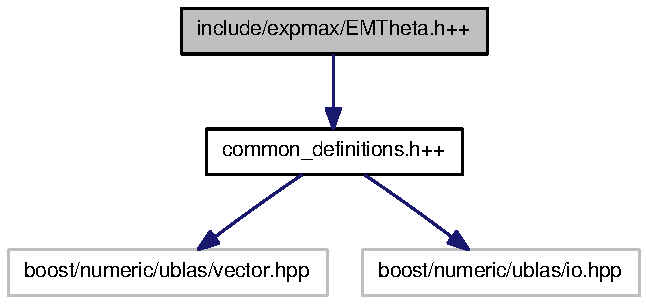
\includegraphics[width=87pt]{EMTheta_8h_09_09__incl}
\end{center}
\end{figure}
Dieser Graph zeigt, welche Datei direkt oder indirekt diese Datei enthält:\nopagebreak
\begin{figure}[H]
\begin{center}
\leavevmode
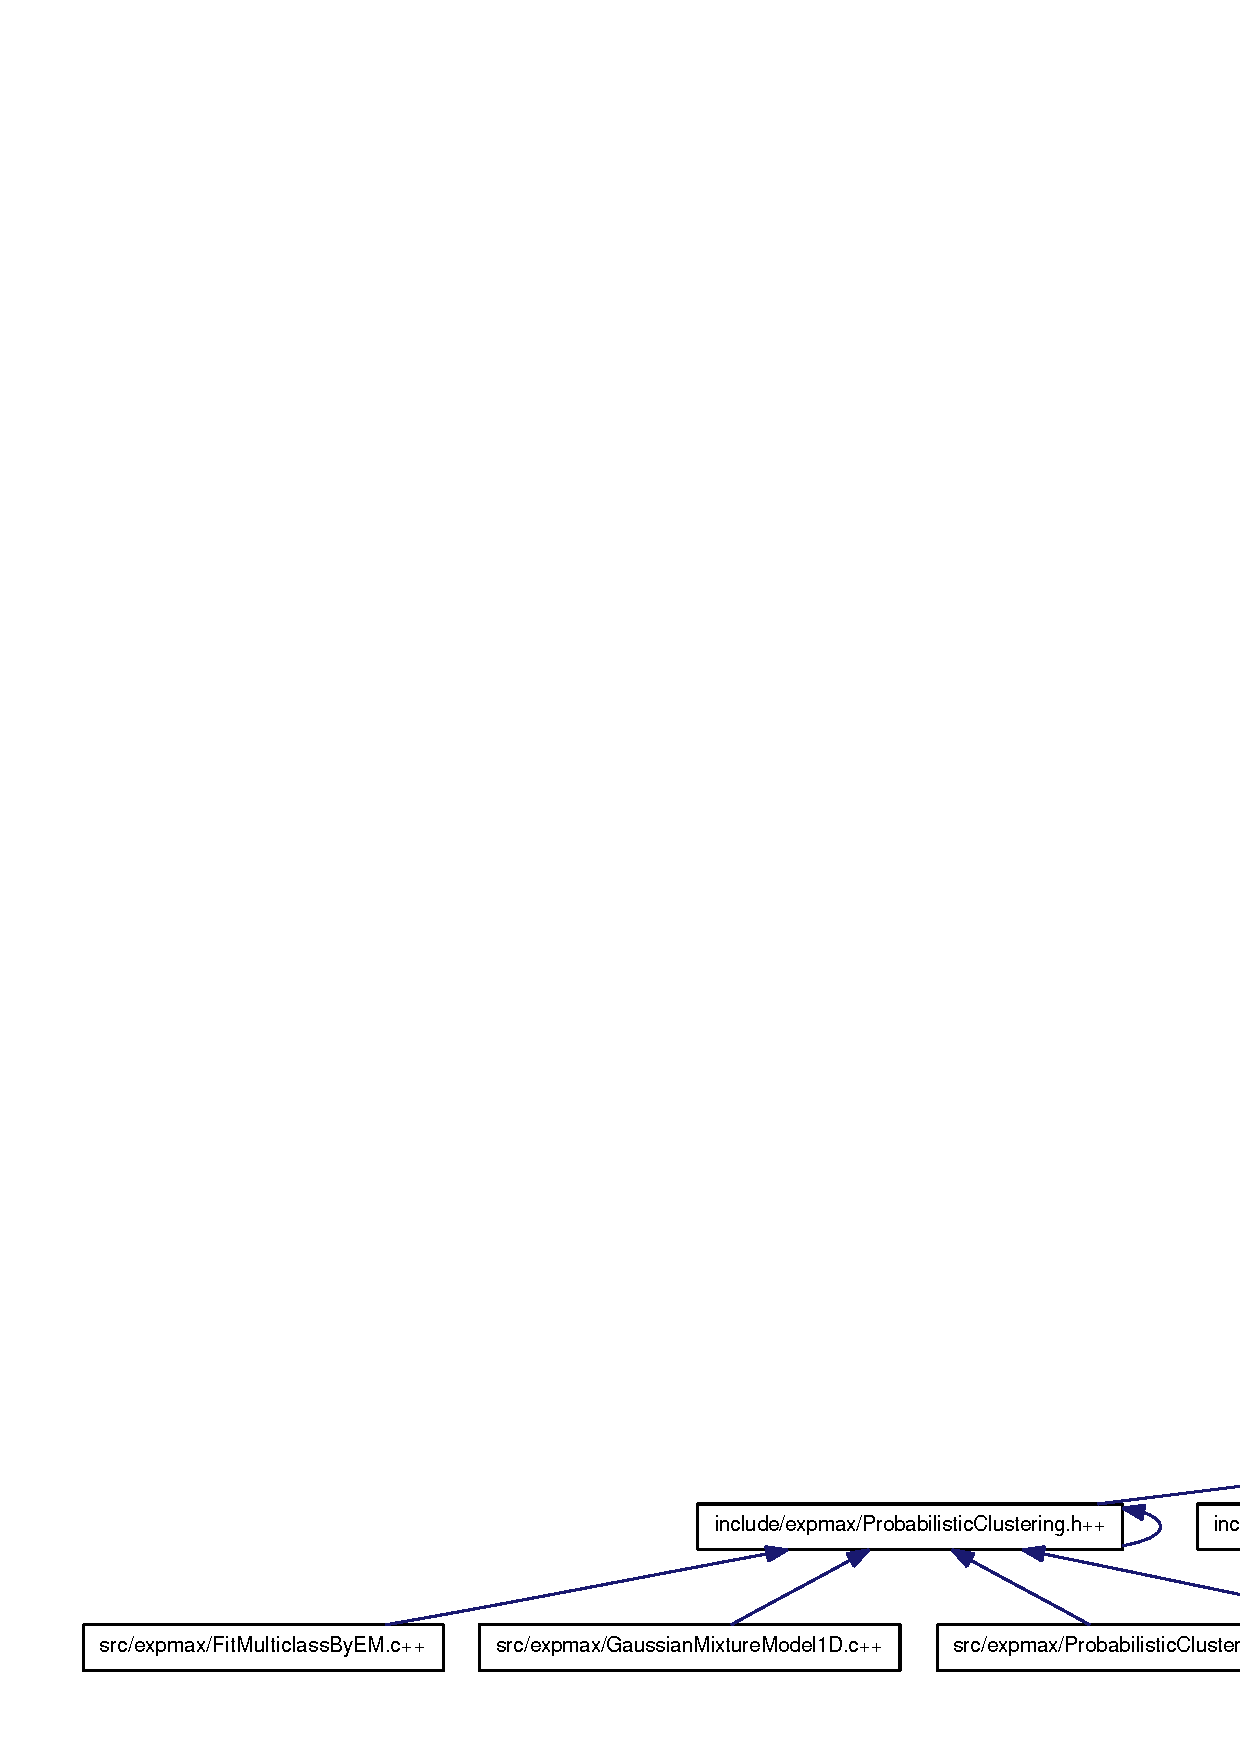
\includegraphics[width=380pt]{EMTheta_8h_09_09__dep__incl}
\end{center}
\end{figure}
\subsection*{Klassen}
\begin{DoxyCompactItemize}
\item 
class \hyperlink{classCDA_1_1EMThetas}{CDA::EMThetas}
\begin{DoxyCompactList}\small\item\em Model parameters for \hyperlink{classCDA_1_1EM}{EM}. \item\end{DoxyCompactList}\end{DoxyCompactItemize}


\subsection{Ausführliche Beschreibung}
\begin{DoxyAuthor}{Autor}
Erik Flick $<$erik.flick \mbox{[}AETT\mbox{]} informatik.uni-\/hamburg.de$>$
\end{DoxyAuthor}
Created on: Jan 5, 2011 
\hypertarget{FitMulticlassByEM_8h_09_09}{
\section{src/expmax/FitMulticlassByEM.h++-\/Dateireferenz}
\label{FitMulticlassByEM_8h_09_09}\index{src/expmax/FitMulticlassByEM.h++@{src/expmax/FitMulticlassByEM.h++}}
}
{\ttfamily \#include \char`\"{}EM.h++\char`\"{}}\par
Include-\/Abhängigkeitsdiagramm für FitMulticlassByEM.h++:\nopagebreak
\begin{figure}[H]
\begin{center}
\leavevmode
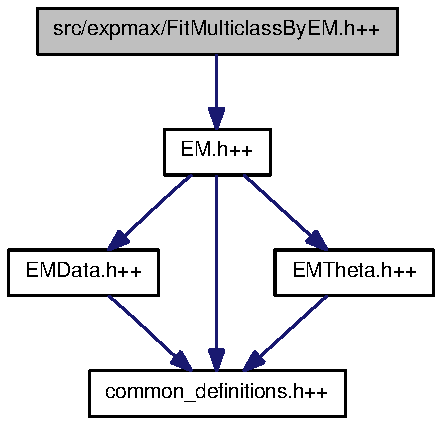
\includegraphics[width=124pt]{FitMulticlassByEM_8h_09_09__incl}
\end{center}
\end{figure}
Dieser Graph zeigt, welche Datei direkt oder indirekt diese Datei enthält:\nopagebreak
\begin{figure}[H]
\begin{center}
\leavevmode
\includegraphics[width=380pt]{FitMulticlassByEM_8h_09_09__dep__incl}
\end{center}
\end{figure}
\subsection*{Klassen}
\begin{DoxyCompactItemize}
\item 
class \hyperlink{classCDA_1_1FitMulticlassByEM}{CDA::FitMulticlassByEM$<$ T $>$}
\end{DoxyCompactItemize}


\subsection{Ausführliche Beschreibung}
\begin{DoxyAuthor}{Autor}
Erik Flick $<$erik.flick \mbox{[}AETT\mbox{]} informatik.uni-\/hamburg.de$>$
\end{DoxyAuthor}
Created on: Jan 5, 2011 
\hypertarget{FitMultivariateMulticlassByEM_8h_09_09}{
\section{src/expmax/FitMultivariateMulticlassByEM.h++-\/Dateireferenz}
\label{FitMultivariateMulticlassByEM_8h_09_09}\index{src/expmax/FitMultivariateMulticlassByEM.h++@{src/expmax/FitMultivariateMulticlassByEM.h++}}
}
{\ttfamily \#include \char`\"{}FitMulticlassByEM.h++\char`\"{}}\par
Include-\/Abhängigkeitsdiagramm für FitMultivariateMulticlassByEM.h++:\nopagebreak
\begin{figure}[H]
\begin{center}
\leavevmode
\includegraphics[width=133pt]{FitMultivariateMulticlassByEM_8h_09_09__incl}
\end{center}
\end{figure}
Dieser Graph zeigt, welche Datei direkt oder indirekt diese Datei enthält:\nopagebreak
\begin{figure}[H]
\begin{center}
\leavevmode
\includegraphics[width=380pt]{FitMultivariateMulticlassByEM_8h_09_09__dep__incl}
\end{center}
\end{figure}
\subsection*{Klassen}
\begin{DoxyCompactItemize}
\item 
class \hyperlink{classCDA_1_1FitMultivariateMulticlassByEM}{CDA::FitMultivariateMulticlassByEM}
\begin{DoxyCompactList}\small\item\em It's been demoted to a typedef. \item\end{DoxyCompactList}\end{DoxyCompactItemize}
\subsection*{Typdefinitionen}
\begin{DoxyCompactItemize}
\item 
\hypertarget{namespaceCDA_ae4a2bfc00d6744ed70526c4cb184ab09}{
typedef FitMulticlassByEM$<$ double $>$ \hyperlink{namespaceCDA_ae4a2bfc00d6744ed70526c4cb184ab09}{CDA::FitUnivariateMulticlassByEM}}
\label{namespaceCDA_ae4a2bfc00d6744ed70526c4cb184ab09}

\begin{DoxyCompactList}\small\item\em It's been demoted to a typedef. \item\end{DoxyCompactList}\end{DoxyCompactItemize}


\subsection{Ausführliche Beschreibung}
\begin{DoxyAuthor}{Autor}
Erik Flick $<$erik.flick \mbox{[}AETT\mbox{]} informatik.uni-\/hamburg.de$>$
\end{DoxyAuthor}
Created on: Jan 5, 2011 
\include{FitUnivariateMulticlassByEM_8h_09_09}
\include{GaussianMixtureModel_8h_09_09}
\hypertarget{GaussianMixtureModel1D_8h_09_09}{
\section{include/expmax/GaussianMixtureModel1D.h++-\/Dateireferenz}
\label{GaussianMixtureModel1D_8h_09_09}\index{include/expmax/GaussianMixtureModel1D.h++@{include/expmax/GaussianMixtureModel1D.h++}}
}
{\ttfamily \#include \char`\"{}FitUnivariateMulticlassByEM.h++\char`\"{}}\par
{\ttfamily \#include \char`\"{}expmax/FitMulticlassByEM.h++\char`\"{}}\par
{\ttfamily \#include $<$boost/function.hpp$>$}\par
Include-\/Abhängigkeitsdiagramm für GaussianMixtureModel1D.h++:\nopagebreak
\begin{figure}[H]
\begin{center}
\leavevmode
\includegraphics[width=365pt]{GaussianMixtureModel1D_8h_09_09__incl}
\end{center}
\end{figure}
Dieser Graph zeigt, welche Datei direkt oder indirekt diese Datei enthält:\nopagebreak
\begin{figure}[H]
\begin{center}
\leavevmode
\includegraphics[width=140pt]{GaussianMixtureModel1D_8h_09_09__dep__incl}
\end{center}
\end{figure}
\subsection*{Klassen}
\begin{DoxyCompactItemize}
\item 
class \hyperlink{classCDA_1_1GaussianMixtureModel1D}{CDA::GaussianMixtureModel1D}
\begin{DoxyCompactList}\small\item\em A \hyperlink{classCDA_1_1GaussianMixtureModel}{GaussianMixtureModel} class, with \hyperlink{classCDA_1_1EM}{EM} fitting routine built in. \item\end{DoxyCompactList}\end{DoxyCompactItemize}


\subsection{Ausführliche Beschreibung}
\begin{DoxyAuthor}{Autor}
Erik Flick $<$erik.flick \mbox{[}AETT\mbox{]} informatik.uni-\/hamburg.de$>$
\end{DoxyAuthor}
Created on: Jan 5, 2011\hypertarget{GaussianMixtureModel1D_8h_09_09_NOTE}{}\subsection{NOTE}\label{GaussianMixtureModel1D_8h_09_09_NOTE}
This one, the easiest one, actually works. 
\include{GaussianMixtureModelNDCommon_8h_09_09}
\include{GaussianMixtureModelNDParams_8h_09_09}
\hypertarget{ProbabilisticClustering_8h_09_09}{
\section{include/expmax/ProbabilisticClustering.h++-\/Dateireferenz}
\label{ProbabilisticClustering_8h_09_09}\index{include/expmax/ProbabilisticClustering.h++@{include/expmax/ProbabilisticClustering.h++}}
}
{\ttfamily \#include $<$typeinfo$>$}\par
{\ttfamily \#include $<$boost/mpl/equal.hpp$>$}\par
{\ttfamily \#include $<$algorithm$>$}\par
{\ttfamily \#include $<$boost/iterator/counting\_\-iterator.hpp$>$}\par
{\ttfamily \#include $<$boost/shared\_\-ptr.hpp$>$}\par
{\ttfamily \#include \char`\"{}GaussianMixtureModel1D.h++\char`\"{}}\par
{\ttfamily \#include \char`\"{}FitUnivariateMulticlassByEM.h++\char`\"{}}\par
{\ttfamily \#include $<$boost/function.hpp$>$}\par
{\ttfamily \#include \char`\"{}expmax/GaussianMixtureModelNDCommon.h++\char`\"{}}\par
{\ttfamily \#include \char`\"{}expmax/FitMultivariateMulticlassByEM.h++\char`\"{}}\par
Include-\/Abhängigkeitsdiagramm für ProbabilisticClustering.h++:\nopagebreak
\begin{figure}[H]
\begin{center}
\leavevmode
\includegraphics[width=420pt]{ProbabilisticClustering_8h_09_09__incl}
\end{center}
\end{figure}
Dieser Graph zeigt, welche Datei direkt oder indirekt diese Datei enthält:\nopagebreak
\begin{figure}[H]
\begin{center}
\leavevmode
\includegraphics[width=398pt]{ProbabilisticClustering_8h_09_09__dep__incl}
\end{center}
\end{figure}


\subsection{Ausführliche Beschreibung}
\begin{DoxyAuthor}{Autor}
Erik Flick $<$erik.flick \mbox{[}AETT\mbox{]} informatik.uni-\/hamburg.de$>$ 
\end{DoxyAuthor}
\begin{DoxyVersion}{Version}
0.1
\end{DoxyVersion}
\hypertarget{ProbabilisticClustering_8c_09_09_LICENSE}{}\subsection{LICENSE}\label{ProbabilisticClustering_8c_09_09_LICENSE}
This file is released under LGPL v3.0.\hypertarget{ProbabilisticClustering_8h_09_09_DESCRIPTION}{}\subsection{DESCRIPTION}\label{ProbabilisticClustering_8h_09_09_DESCRIPTION}
Gaussian Mixture Model for fitting of a known number of Gaussians; and other probabilistic models of use in the processing of images.

Common patterns are extracted afap to build a hierarchy of classes. 
\include{utilities_8h_09_09}
\include{VectorEMData_8h_09_09}
\hypertarget{CircularStatistics_8h_09_09}{
\section{include/math/CircularStatistics.h++-\/Dateireferenz}
\label{CircularStatistics_8h_09_09}\index{include/math/CircularStatistics.h++@{include/math/CircularStatistics.h++}}
}


Special functions for circular statistics.  


{\ttfamily \#include $<$gsl/gsl\_\-sf\_\-bessel.h$>$}\par
{\ttfamily \#include $<$cmath$>$}\par
Include-\/Abhängigkeitsdiagramm für CircularStatistics.h++:\nopagebreak
\begin{figure}[H]
\begin{center}
\leavevmode
\includegraphics[width=111pt]{CircularStatistics_8h_09_09__incl}
\end{center}
\end{figure}
Dieser Graph zeigt, welche Datei direkt oder indirekt diese Datei enthält:\nopagebreak
\begin{figure}[H]
\begin{center}
\leavevmode
\includegraphics[width=258pt]{CircularStatistics_8h_09_09__dep__incl}
\end{center}
\end{figure}
\subsection*{Klassen}
\begin{DoxyCompactItemize}
\item 
struct \hyperlink{structCDA_1_1VonMises}{CDA::VonMises}
\end{DoxyCompactItemize}
\subsection*{Funktionen}
\begin{DoxyCompactItemize}
\item 
\hypertarget{CircularStatistics_8h_09_09_a53bb96d37a7af4fd27ce73a33a69c63a}{
double {\bfseries wrap2pi} (const double phi)}
\label{CircularStatistics_8h_09_09_a53bb96d37a7af4fd27ce73a33a69c63a}

\end{DoxyCompactItemize}


\subsection{Ausführliche Beschreibung}
Special functions for circular statistics. \begin{DoxyAuthor}{Autor}
Erik Flick $<$erik.flick \mbox{[}AETT\mbox{]} informatik.uni-\/hamburg.de$>$
\end{DoxyAuthor}
Created on: Dec 28, 2010 
\include{matrix__functions_8h_09_09}
\hypertarget{numeric__optimization_8h_09_09}{
\section{include/math/numeric\_\-optimization.h++-\/Dateireferenz}
\label{numeric__optimization_8h_09_09}\index{include/math/numeric\_\-optimization.h++@{include/math/numeric\_\-optimization.h++}}
}
{\ttfamily \#include $<$boost/function.hpp$>$}\par
Include-\/Abhängigkeitsdiagramm für numeric\_\-optimization.h++:\nopagebreak
\begin{figure}[H]
\begin{center}
\leavevmode
\includegraphics[width=115pt]{numeric__optimization_8h_09_09__incl}
\end{center}
\end{figure}
Dieser Graph zeigt, welche Datei direkt oder indirekt diese Datei enthält:\nopagebreak
\begin{figure}[H]
\begin{center}
\leavevmode
\includegraphics[width=123pt]{numeric__optimization_8h_09_09__dep__incl}
\end{center}
\end{figure}
\subsection*{Funktionen}
\begin{DoxyCompactItemize}
\item 
double \hyperlink{namespaceCDA_ab4d6ad3bb6730a396ee12d33fe5ad7ca}{CDA::findSingleUnivariateRootIntervalSearch} (const boost::function$<$ double(double)$>$ \&f, const double xa, const double xb, const double epsilon)
\begin{DoxyCompactList}\small\item\em Finds one root in the given interval. \item\end{DoxyCompactList}\end{DoxyCompactItemize}


\subsection{Ausführliche Beschreibung}
\begin{DoxyVersion}{Version}
0.01 
\end{DoxyVersion}
\begin{DoxyAuthor}{Autor}
Erik Flick $<$erik.flick \mbox{[}AETT\mbox{]} informatik.uni-\/hamburg.de$>$
\end{DoxyAuthor}
Created on: Dec 28, 2010 
\hypertarget{comparisons_8h_09_09}{
\section{include/utils/comparisons.h++-\/Dateireferenz}
\label{comparisons_8h_09_09}\index{include/utils/comparisons.h++@{include/utils/comparisons.h++}}
}
Dieser Graph zeigt, welche Datei direkt oder indirekt diese Datei enthält:\nopagebreak
\begin{figure}[H]
\begin{center}
\leavevmode
\includegraphics[width=226pt]{comparisons_8h_09_09__dep__incl}
\end{center}
\end{figure}
\subsection*{Klassen}
\begin{DoxyCompactItemize}
\item 
class \hyperlink{structCDA_1_1compareByVectorElementValue}{CDA::compareByVectorElementValue$<$ vector\_\-t, idx\_\-t, LT $>$}
\begin{DoxyCompactList}\small\item\em Use this as a {\bfseries functor} to compare numbers a and b by the values v\mbox{[}a\mbox{]} and v\mbox{[}b\mbox{]}. \item\end{DoxyCompactList}\end{DoxyCompactItemize}


\subsection{Ausführliche Beschreibung}
\begin{DoxyAuthor}{Autor}
Erik Flick $<$erik.flick \mbox{[}AETT\mbox{]} informatik.uni-\/hamburg.de$>$
\end{DoxyAuthor}
Created on: Dec 29, 2010 
\include{EM_8c_09_09}
\include{EMData_8c_09_09}
\include{EMGenericMixtureModelCore_8c_09_09}
\include{EMTheta_8c_09_09}
\include{FitMulticlassByEM_8c_09_09}
\include{FitMultivariateMulticlassByEM_8c_09_09}
\include{GaussianMixtureModel_8c_09_09}
\include{GaussianMixtureModel1D_8c_09_09}
\include{GaussianMixtureModelNDCommon_8c_09_09}
\include{GaussianMixtureModelNDParams_8c_09_09}
\hypertarget{ProbabilisticClustering_8c_09_09}{
\section{src/expmax/ProbabilisticClustering.c++-\/Dateireferenz}
\label{ProbabilisticClustering_8c_09_09}\index{src/expmax/ProbabilisticClustering.c++@{src/expmax/ProbabilisticClustering.c++}}
}
{\ttfamily \#include \char`\"{}ProbabilisticClustering.h++\char`\"{}}\par
{\ttfamily \#include $<$typeinfo$>$}\par
{\ttfamily \#include $<$boost/foreach.hpp$>$}\par
{\ttfamily \#include $<$boost/optional.hpp$>$}\par
{\ttfamily \#include $<$boost/mpl/equal.hpp$>$}\par
{\ttfamily \#include $<$boost/function.hpp$>$}\par
{\ttfamily \#include $<$boost/lambda/bind.hpp$>$}\par
{\ttfamily \#include $<$boost/lambda/lambda.hpp$>$}\par
{\ttfamily \#include $<$algorithm$>$}\par
{\ttfamily \#include $<$boost/iterator/counting\_\-iterator.hpp$>$}\par
{\ttfamily \#include $<$boost/algorithm/minmax\_\-element.hpp$>$}\par
{\ttfamily \#include $<$boost/shared\_\-ptr.hpp$>$}\par
{\ttfamily \#include $<$boost/numeric/ublas/matrix.hpp$>$}\par
{\ttfamily \#include $<$boost/numeric/ublas/symmetric.hpp$>$}\par
{\ttfamily \#include $<$boost/numeric/ublas/vector.hpp$>$}\par
{\ttfamily \#include $<$boost/numeric/ublas/vector\_\-proxy.hpp$>$}\par
{\ttfamily \#include $<$boost/numeric/ublas/io.hpp$>$}\par
{\ttfamily \#include $<$boost/numeric/ublas/lu.hpp$>$}\par
{\ttfamily \#include $<$limits$>$}\par
{\ttfamily \#include $<$iostream$>$}\par
{\ttfamily \#include \char`\"{}math/CircularStatistics.h++\char`\"{}}\par
{\ttfamily \#include \char`\"{}math/numeric\_\-optimization.h++\char`\"{}}\par
{\ttfamily \#include \char`\"{}utils/comparisons.h++\char`\"{}}\par
{\ttfamily \#include \char`\"{}common\_\-definitions.h++\char`\"{}}\par
{\ttfamily \#include \char`\"{}FitMultivariateMulticlassByEM.h++\char`\"{}}\par
{\ttfamily \#include \char`\"{}EMGenericMixtureModelCore.h++\char`\"{}}\par
{\ttfamily \#include \char`\"{}EMCustomOptimization.h++\char`\"{}}\par
{\ttfamily \#include $<$sstream$>$}\par
{\ttfamily \#include $<$boost/numeric/ublas/triangular.hpp$>$}\par
Include-\/Abhängigkeitsdiagramm für ProbabilisticClustering.c++:\nopagebreak
\begin{figure}[H]
\begin{center}
\leavevmode
\includegraphics[width=420pt]{ProbabilisticClustering_8c_09_09__incl}
\end{center}
\end{figure}
Dieser Graph zeigt, welche Datei direkt oder indirekt diese Datei enthält:\nopagebreak
\begin{figure}[H]
\begin{center}
\leavevmode
\includegraphics[width=124pt]{ProbabilisticClustering_8c_09_09__dep__incl}
\end{center}
\end{figure}


\subsection{Ausführliche Beschreibung}
\begin{DoxyAuthor}{Autor}
Erik Flick $<$erik.flick \mbox{[}AETT\mbox{]} informatik.uni-\/hamburg.de$>$ 
\end{DoxyAuthor}
\begin{DoxyVersion}{Version}
0.1
\end{DoxyVersion}
\hypertarget{ProbabilisticClustering_8h_09_09_LICENSE}{}\subsection{LICENSE}\label{ProbabilisticClustering_8h_09_09_LICENSE}
This file is released under LGPL v3.0.

Created on: Dec 16, 2010

\begin{Desc}
\item[\hyperlink{todo__todo000007}{Noch zu erledigen}]crippling bugs in multivariate gaussian specialization\end{Desc}

\include{VectorEMData_8c_09_09}
\hypertarget{CircularStatistics_8c_09_09}{
\section{include/math/CircularStatistics.c++-\/Dateireferenz}
\label{CircularStatistics_8c_09_09}\index{include/math/CircularStatistics.c++@{include/math/CircularStatistics.c++}}
}
{\ttfamily \#include \char`\"{}CircularStatistics.h++\char`\"{}}\par
{\ttfamily \#include $<$gsl/gsl\_\-sf\_\-bessel.h$>$}\par
{\ttfamily \#include $<$cmath$>$}\par
Include-\/Abhängigkeitsdiagramm für CircularStatistics.c++:\nopagebreak
\begin{figure}[H]
\begin{center}
\leavevmode
\includegraphics[width=120pt]{CircularStatistics_8c_09_09__incl}
\end{center}
\end{figure}
Dieser Graph zeigt, welche Datei direkt oder indirekt diese Datei enthält:\nopagebreak
\begin{figure}[H]
\begin{center}
\leavevmode
\includegraphics[width=115pt]{CircularStatistics_8c_09_09__dep__incl}
\end{center}
\end{figure}
\subsection*{Funktionen}
\begin{DoxyCompactItemize}
\item 
\hypertarget{CircularStatistics_8c_09_09_a53bb96d37a7af4fd27ce73a33a69c63a}{
double {\bfseries wrap2pi} (const double phi)}
\label{CircularStatistics_8c_09_09_a53bb96d37a7af4fd27ce73a33a69c63a}

\end{DoxyCompactItemize}


\subsection{Ausführliche Beschreibung}
\begin{DoxyAuthor}{Autor}
Erik Flick $<$erik.flick \mbox{[}AETT\mbox{]} informatik.uni-\/hamburg.de$>$
\end{DoxyAuthor}
Created on: Jan 5, 2011 
\hypertarget{numeric__optimization_8c_09_09}{
\section{src/math/numeric\_\-optimization.c++-\/Dateireferenz}
\label{numeric__optimization_8c_09_09}\index{src/math/numeric\_\-optimization.c++@{src/math/numeric\_\-optimization.c++}}
}
{\ttfamily \#include \char`\"{}include/math/numeric\_\-optimization.h++\char`\"{}}\par
{\ttfamily \#include $<$boost/function.hpp$>$}\par
Include-\/Abhängigkeitsdiagramm für numeric\_\-optimization.c++:\nopagebreak
\begin{figure}[H]
\begin{center}
\leavevmode
\includegraphics[width=116pt]{numeric__optimization_8c_09_09__incl}
\end{center}
\end{figure}
Dieser Graph zeigt, welche Datei direkt oder indirekt diese Datei enthält:\nopagebreak
\begin{figure}[H]
\begin{center}
\leavevmode
\includegraphics[width=116pt]{numeric__optimization_8c_09_09__dep__incl}
\end{center}
\end{figure}
\subsection*{Funktionen}
\begin{DoxyCompactItemize}
\item 
double \hyperlink{namespaceCDA_ab4d6ad3bb6730a396ee12d33fe5ad7ca}{CDA::findSingleUnivariateRootIntervalSearch} (const boost::function$<$ double(double)$>$ \&f, const double xa, const double xb, const double epsilon)
\begin{DoxyCompactList}\small\item\em Finds one root in the given interval. \item\end{DoxyCompactList}\end{DoxyCompactItemize}


\subsection{Ausführliche Beschreibung}
\begin{DoxyAuthor}{Autor}
Erik Flick $<$erik.flick \mbox{[}AETT\mbox{]} informatik.uni-\/hamburg.de$>$
\end{DoxyAuthor}
Created on: Dec 28, 2010 
\printindex
\end{document}
